\documentclass[twoside]{book}

% Packages required by doxygen
\usepackage{calc}
\usepackage{doxygen}
\usepackage{graphicx}
\usepackage[utf8]{inputenc}
\usepackage{makeidx}
\usepackage{multicol}
\usepackage{multirow}
\usepackage{textcomp}
\usepackage[table]{xcolor}

% Font selection
\usepackage[T1]{fontenc}
\usepackage{mathptmx}
\usepackage[scaled=.90]{helvet}
\usepackage{courier}
\usepackage{amssymb}
\usepackage{sectsty}
\renewcommand{\familydefault}{\sfdefault}
\allsectionsfont{%
  \fontseries{bc}\selectfont%
  \color{darkgray}%
}
\renewcommand{\DoxyLabelFont}{%
  \fontseries{bc}\selectfont%
  \color{darkgray}%
}

% Page & text layout
\usepackage{geometry}
\geometry{%
  a4paper,%
  top=2.5cm,%
  bottom=2.5cm,%
  left=2.5cm,%
  right=2.5cm%
}
\tolerance=750
\hfuzz=15pt
\hbadness=750
\setlength{\emergencystretch}{15pt}
\setlength{\parindent}{0cm}
\setlength{\parskip}{0.2cm}
\makeatletter
\renewcommand{\paragraph}{%
  \@startsection{paragraph}{4}{0ex}{-1.0ex}{1.0ex}{%
    \normalfont\normalsize\bfseries\SS@parafont%
  }%
}
\renewcommand{\subparagraph}{%
  \@startsection{subparagraph}{5}{0ex}{-1.0ex}{1.0ex}{%
    \normalfont\normalsize\bfseries\SS@subparafont%
  }%
}
\makeatother

% Headers & footers
\usepackage{fancyhdr}
\pagestyle{fancyplain}
\fancyhead[LE]{\fancyplain{}{\bfseries\thepage}}
\fancyhead[CE]{\fancyplain{}{}}
\fancyhead[RE]{\fancyplain{}{\bfseries\leftmark}}
\fancyhead[LO]{\fancyplain{}{\bfseries\rightmark}}
\fancyhead[CO]{\fancyplain{}{}}
\fancyhead[RO]{\fancyplain{}{\bfseries\thepage}}
\fancyfoot[LE]{\fancyplain{}{}}
\fancyfoot[CE]{\fancyplain{}{}}
\fancyfoot[RE]{\fancyplain{}{\bfseries\scriptsize Generated on Tue Oct 22 2013 18\-:21\-:59 for D\-D\-T by Doxygen }}
\fancyfoot[LO]{\fancyplain{}{\bfseries\scriptsize Generated on Tue Oct 22 2013 18\-:21\-:59 for D\-D\-T by Doxygen }}
\fancyfoot[CO]{\fancyplain{}{}}
\fancyfoot[RO]{\fancyplain{}{}}
\renewcommand{\footrulewidth}{0.4pt}
\renewcommand{\chaptermark}[1]{%
  \markboth{#1}{}%
}
\renewcommand{\sectionmark}[1]{%
  \markright{\thesection\ #1}%
}

% Indices & bibliography
\usepackage{natbib}
\usepackage[titles]{tocloft}
\setcounter{tocdepth}{3}
\setcounter{secnumdepth}{5}
\makeindex

% Hyperlinks (required, but should be loaded last)
\usepackage{ifpdf}
\ifpdf
  \usepackage[pdftex,pagebackref=true]{hyperref}
\else
  \usepackage[ps2pdf,pagebackref=true]{hyperref}
\fi
\hypersetup{%
  colorlinks=true,%
  linkcolor=blue,%
  citecolor=blue,%
  unicode%
}

% Custom commands
\newcommand{\clearemptydoublepage}{%
  \newpage{\pagestyle{empty}\cleardoublepage}%
}


%===== C O N T E N T S =====

\begin{document}

% Titlepage & ToC
\hypersetup{pageanchor=false}
\pagenumbering{roman}
\begin{titlepage}
\vspace*{7cm}
\begin{center}%
{\Large D\-D\-T }\\
\vspace*{1cm}
{\large Generated by Doxygen 1.8.5}\\
\vspace*{0.5cm}
{\small Tue Oct 22 2013 18:21:59}\\
\end{center}
\end{titlepage}
\clearemptydoublepage
\tableofcontents
\clearemptydoublepage
\pagenumbering{arabic}
\hypersetup{pageanchor=true}

%--- Begin generated contents ---
\chapter{Hierarchical Index}
\section{Class Hierarchy}
This inheritance list is sorted roughly, but not completely, alphabetically\-:\begin{DoxyCompactList}
\item Application\-Window\begin{DoxyCompactList}
\item \contentsline{section}{main}{\pageref{classmain}}{}
\end{DoxyCompactList}
\item \contentsline{section}{D\-D\-T\-Configuration}{\pageref{classDDTConfiguration}}{}
\item Focus\-Scope\begin{DoxyCompactList}
\item \contentsline{section}{Auto\-Complete\-Text\-Field}{\pageref{classAutoCompleteTextField}}{}
\item \contentsline{section}{Focus\-And\-Edit\-Text\-Field}{\pageref{classFocusAndEditTextField}}{}
\end{DoxyCompactList}
\item Grid\begin{DoxyCompactList}
\item \contentsline{section}{Allowed\-Roles\-Editor}{\pageref{classAllowedRolesEditor}}{}
\end{DoxyCompactList}
\item Item\begin{DoxyCompactList}
\item \contentsline{section}{Debate\-Page}{\pageref{classDebatePage}}{}
\item \contentsline{section}{Table}{\pageref{classTable}}{}
\item \contentsline{section}{Tri\-Cell}{\pageref{classTriCell}}{}
\end{DoxyCompactList}
\item List\-View\begin{DoxyCompactList}
\item \contentsline{section}{Speaker\-List}{\pageref{classSpeakerList}}{}
\item \contentsline{section}{Team\-Editor}{\pageref{classTeamEditor}}{}
\end{DoxyCompactList}
\item Q\-Abstract\-List\-Model\begin{DoxyCompactList}
\item \contentsline{section}{Q\-List\-Qml\-Wrapper}{\pageref{classQListQmlWrapper}}{}
\begin{DoxyCompactList}
\item \contentsline{section}{Prototype\-Q\-List\-Qml\-Wrapper}{\pageref{classPrototypeQListQmlWrapper}}{}
\end{DoxyCompactList}
\end{DoxyCompactList}
\item Q\-Object\begin{DoxyCompactList}
\item \contentsline{section}{Auto\-Complete\-Model}{\pageref{classAutoCompleteModel}}{}
\item \contentsline{section}{Debate}{\pageref{classDebate}}{}
\begin{DoxyCompactList}
\item \contentsline{section}{B\-P\-S\-Debate}{\pageref{classBPSDebate}}{}
\item \contentsline{section}{O\-P\-Debate}{\pageref{classOPDebate}}{}
\end{DoxyCompactList}
\item \contentsline{section}{Main\-Model}{\pageref{classMainModel}}{}
\item \contentsline{section}{Matching\-Solver}{\pageref{classMatchingSolver}}{}
\item \contentsline{section}{Mixed\-Value\-Speaker\-Model}{\pageref{classMixedValueSpeakerModel}}{}
\item \contentsline{section}{Seat\-To\-Speaker\-Mapper}{\pageref{classSeatToSpeakerMapper}}{}
\item \contentsline{section}{Speaker\-Model}{\pageref{classSpeakerModel}}{}
\item \contentsline{section}{Table\-Names}{\pageref{classTableNames}}{}
\item \contentsline{section}{Team}{\pageref{classTeam}}{}
\end{DoxyCompactList}
\item Rectangle\begin{DoxyCompactList}
\item \contentsline{section}{B\-P\-S\-Debate\-View}{\pageref{classBPSDebateView}}{}
\item \contentsline{section}{H\-Bar}{\pageref{classHBar}}{}
\item \contentsline{section}{O\-P\-D\-Debate\-View}{\pageref{classOPDDebateView}}{}
\item \contentsline{section}{Result\-Page}{\pageref{classResultPage}}{}
\item \contentsline{section}{Round\-Button}{\pageref{classRoundButton}}{}
\item \contentsline{section}{Speaker\-Page}{\pageref{classSpeakerPage}}{}
\end{DoxyCompactList}
\item \contentsline{section}{Role\-Link}{\pageref{structRoleLink}}{}
\item Search\-Monitor\begin{DoxyCompactList}
\item \contentsline{section}{Interrupt\-Handler}{\pageref{classInterruptHandler}}{}
\end{DoxyCompactList}
\end{DoxyCompactList}

\chapter{Class Index}
\section{Class List}
Here are the classes, structs, unions and interfaces with brief descriptions\-:\begin{DoxyCompactList}
\item\contentsline{section}{\hyperlink{classAllowedRolesEditor}{Allowed\-Roles\-Editor} \\*An editor used to edit the allowed roles of a one ore more speakers }{\pageref{classAllowedRolesEditor}}{}
\item\contentsline{section}{\hyperlink{classAutoCompleteModel}{Auto\-Complete\-Model} \\*Offers autocompletion accessible from Q\-M\-L }{\pageref{classAutoCompleteModel}}{}
\item\contentsline{section}{\hyperlink{classAutoCompleteTextField}{Auto\-Complete\-Text\-Field} \\*A text field with autocompletion }{\pageref{classAutoCompleteTextField}}{}
\item\contentsline{section}{\hyperlink{classBPSDebate}{B\-P\-S\-Debate} \\*Represents a debate in B\-P\-S-\/format }{\pageref{classBPSDebate}}{}
\item\contentsline{section}{\hyperlink{classBPSDebateView}{B\-P\-S\-Debate\-View} \\*Displays a B\-P\-S debate }{\pageref{classBPSDebateView}}{}
\item\contentsline{section}{\hyperlink{classDDTConfiguration}{D\-D\-T\-Configuration} \\*Reads options from a file }{\pageref{classDDTConfiguration}}{}
\item\contentsline{section}{\hyperlink{classDebate}{Debate} \\*Represents an abstract debate }{\pageref{classDebate}}{}
\item\contentsline{section}{\hyperlink{classDebatePage}{Debate\-Page} \\*Displays a component that allows editing the applications debate's }{\pageref{classDebatePage}}{}
\item\contentsline{section}{\hyperlink{classFocusAndEditTextField}{Focus\-And\-Edit\-Text\-Field} }{\pageref{classFocusAndEditTextField}}{}
\item\contentsline{section}{\hyperlink{classHBar}{H\-Bar} \\*A simple gray horizontal bar, can be used to split different elements }{\pageref{classHBar}}{}
\item\contentsline{section}{\hyperlink{classInterruptHandler}{Interrupt\-Handler} }{\pageref{classInterruptHandler}}{}
\item\contentsline{section}{\hyperlink{classmain}{main} \\*D\-D\-T's one and only application window }{\pageref{classmain}}{}
\item\contentsline{section}{\hyperlink{classMainModel}{Main\-Model} \\*Offers access to all parts of the application's model }{\pageref{classMainModel}}{}
\item\contentsline{section}{\hyperlink{classMatchingSolver}{Matching\-Solver} \\*Solves the main D\-D\-T matching problem }{\pageref{classMatchingSolver}}{}
\item\contentsline{section}{\hyperlink{classMixedValueSpeakerModel}{Mixed\-Value\-Speaker\-Model} \\*Allows editing multiple speakers at once }{\pageref{classMixedValueSpeakerModel}}{}
\item\contentsline{section}{\hyperlink{classOPDDebateView}{O\-P\-D\-Debate\-View} \\*Displays an O\-P debate }{\pageref{classOPDDebateView}}{}
\item\contentsline{section}{\hyperlink{classOPDebate}{O\-P\-Debate} \\*Represents a debate in O\-P\-D-\/format }{\pageref{classOPDebate}}{}
\item\contentsline{section}{\hyperlink{classPrototypeQListQmlWrapper}{Prototype\-Q\-List\-Qml\-Wrapper} \\*A \hyperlink{classQListQmlWrapper}{Q\-List\-Qml\-Wrapper} with roles extrated from a prototype object }{\pageref{classPrototypeQListQmlWrapper}}{}
\item\contentsline{section}{\hyperlink{classQListQmlWrapper}{Q\-List\-Qml\-Wrapper} \\*Allows accessing a cpp list in Q\-M\-L }{\pageref{classQListQmlWrapper}}{}
\item\contentsline{section}{\hyperlink{classResultPage}{Result\-Page} }{\pageref{classResultPage}}{}
\item\contentsline{section}{\hyperlink{structRoleLink}{Role\-Link} }{\pageref{structRoleLink}}{}
\item\contentsline{section}{\hyperlink{classRoundButton}{Round\-Button} }{\pageref{classRoundButton}}{}
\item\contentsline{section}{\hyperlink{classSeatToSpeakerMapper}{Seat\-To\-Speaker\-Mapper} \\*Represents the results of a matching process }{\pageref{classSeatToSpeakerMapper}}{}
\item\contentsline{section}{\hyperlink{classSpeakerList}{Speaker\-List} }{\pageref{classSpeakerList}}{}
\item\contentsline{section}{\hyperlink{classSpeakerModel}{Speaker\-Model} \\*Represents a speaker in a debate }{\pageref{classSpeakerModel}}{}
\item\contentsline{section}{\hyperlink{classSpeakerPage}{Speaker\-Page} \\*A component that allows the selection and editing of on ore more speakers }{\pageref{classSpeakerPage}}{}
\item\contentsline{section}{\hyperlink{classTable}{Table} \\*Displays a debate's table and all enabled team seats }{\pageref{classTable}}{}
\item\contentsline{section}{\hyperlink{classTableNames}{Table\-Names} \\*Stores speakers mapped to a table in a debate }{\pageref{classTableNames}}{}
\item\contentsline{section}{\hyperlink{classTeam}{Team} \\*Represents a team in a debate }{\pageref{classTeam}}{}
\item\contentsline{section}{\hyperlink{classTeamEditor}{Team\-Editor} \\*An editor allowing the editing of teams }{\pageref{classTeamEditor}}{}
\item\contentsline{section}{\hyperlink{classTriCell}{Tri\-Cell} \\*A styled cell with three different possible states }{\pageref{classTriCell}}{}
\end{DoxyCompactList}

\chapter{Class Documentation}
\hypertarget{classAllowedRolesEditor}{\section{Allowed\-Roles\-Editor Class Reference}
\label{classAllowedRolesEditor}\index{Allowed\-Roles\-Editor@{Allowed\-Roles\-Editor}}
}


An editor used to edit the allowed roles of a one ore more speakers.  


Inheritance diagram for Allowed\-Roles\-Editor\-:\begin{figure}[H]
\begin{center}
\leavevmode
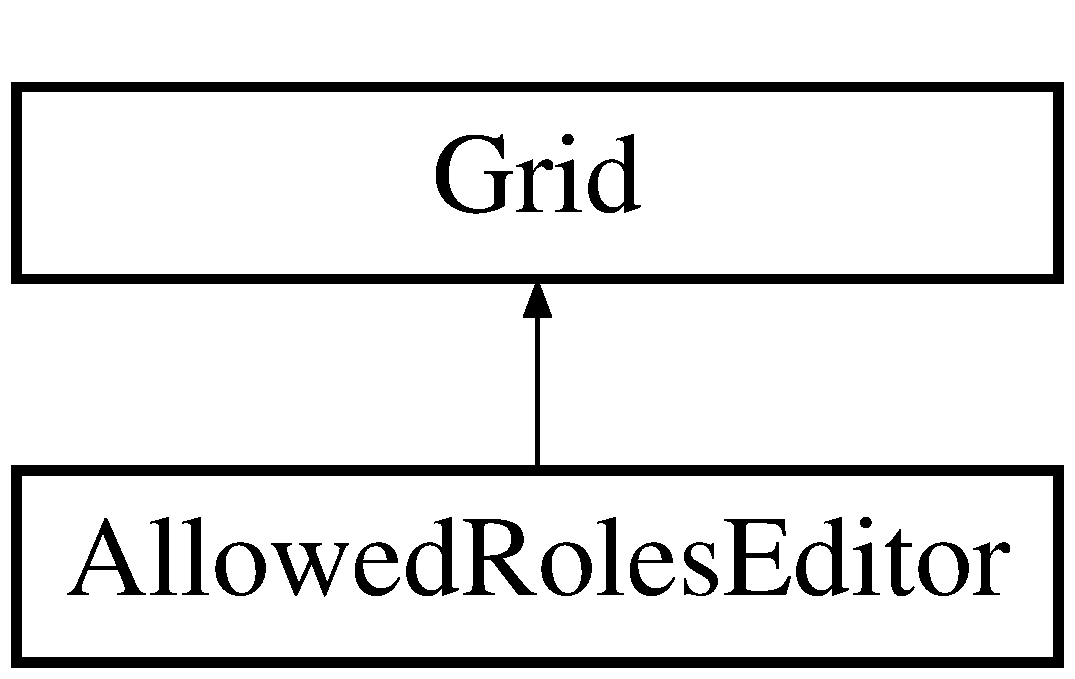
\includegraphics[height=2.000000cm]{classAllowedRolesEditor}
\end{center}
\end{figure}
\subsection*{Properties}
\begin{DoxyCompactItemize}
\item 
\hypertarget{classAllowedRolesEditor_a86e4e22c541f8fefd3a72d7b0b281749}{\hyperlink{classMixedValueSpeakerModel}{Mixed\-Value\-Speaker\-Model} \hyperlink{classAllowedRolesEditor_a86e4e22c541f8fefd3a72d7b0b281749}{mixed\-Model}}\label{classAllowedRolesEditor_a86e4e22c541f8fefd3a72d7b0b281749}

\begin{DoxyCompactList}\small\item\em The editors model. \end{DoxyCompactList}\end{DoxyCompactItemize}


\subsection{Detailed Description}
An editor used to edit the allowed roles of a one ore more speakers. 

The editor allows easy and fast editing of some speakers allowed roles. If some speakers have different property values, a mixed value will be shown. Editing will set a property of all speakers to the same value. \begin{DoxySeeAlso}{See Also}
\hyperlink{classSpeakerModel}{Speaker\-Model} \hyperlink{classMixedValueSpeakerModel}{Mixed\-Value\-Speaker\-Model} 
\end{DoxySeeAlso}


The documentation for this class was generated from the following file\-:\begin{DoxyCompactItemize}
\item 
/home/stoef/qt/projects/ddt/ddt/qml/ddt/Allowed\-Roles\-Editor.\-qml\end{DoxyCompactItemize}

\hypertarget{classAutoCompleteModel}{\section{Auto\-Complete\-Model Class Reference}
\label{classAutoCompleteModel}\index{Auto\-Complete\-Model@{Auto\-Complete\-Model}}
}


Offers autocompletion accessible from Q\-M\-L.  




{\ttfamily \#include $<$autocompletemodel.\-h$>$}

Inheritance diagram for Auto\-Complete\-Model\-:\begin{figure}[H]
\begin{center}
\leavevmode
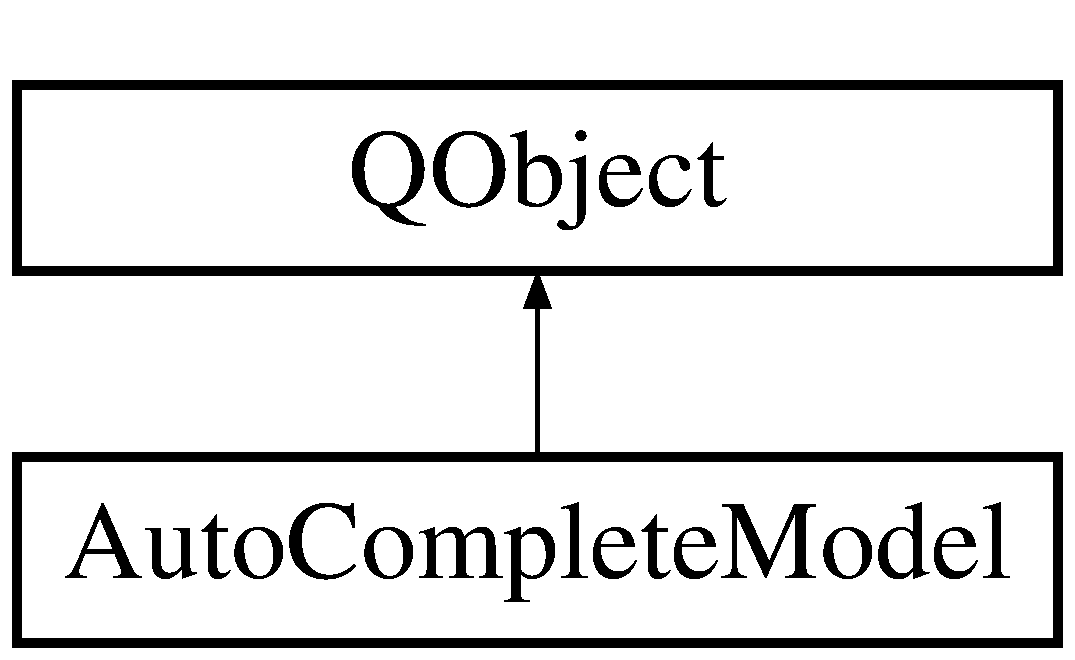
\includegraphics[height=2.000000cm]{classAutoCompleteModel}
\end{center}
\end{figure}
\subsection*{Public Member Functions}
\begin{DoxyCompactItemize}
\item 
\hyperlink{classAutoCompleteModel_ae7c8421f60a6602bf43e11199c69a130}{Auto\-Complete\-Model} (Q\-String\-List $\ast$list=0, Q\-Object $\ast$parent=0)
\begin{DoxyCompactList}\small\item\em Creates a new {\ttfamily \hyperlink{classAutoCompleteModel}{Auto\-Complete\-Model}} with a given list of completions. \end{DoxyCompactList}\item 
Q\-\_\-\-I\-N\-V\-O\-K\-A\-B\-L\-E Q\-String\-List \hyperlink{classAutoCompleteModel_a4f7f2ee3af6dd85e26158a280d933a86}{completions} (Q\-String prefix)
\begin{DoxyCompactList}\small\item\em Returns a list of possible completions for a given search term. \end{DoxyCompactList}\end{DoxyCompactItemize}


\subsection{Detailed Description}
Offers autocompletion accessible from Q\-M\-L. 

Offers simple auto completion functions similar to Q\-Completer that can be accessed from Q\-M\-L. The pool of possible completions is stored a Q\-String\-List . 

\subsection{Constructor \& Destructor Documentation}
\hypertarget{classAutoCompleteModel_ae7c8421f60a6602bf43e11199c69a130}{\index{Auto\-Complete\-Model@{Auto\-Complete\-Model}!Auto\-Complete\-Model@{Auto\-Complete\-Model}}
\index{Auto\-Complete\-Model@{Auto\-Complete\-Model}!AutoCompleteModel@{Auto\-Complete\-Model}}
\subsubsection[{Auto\-Complete\-Model}]{\setlength{\rightskip}{0pt plus 5cm}Auto\-Complete\-Model\-::\-Auto\-Complete\-Model (
\begin{DoxyParamCaption}
\item[{Q\-String\-List $\ast$}]{list = {\ttfamily 0}, }
\item[{Q\-Object $\ast$}]{parent = {\ttfamily 0}}
\end{DoxyParamCaption}
)\hspace{0.3cm}{\ttfamily [explicit]}}}\label{classAutoCompleteModel_ae7c8421f60a6602bf43e11199c69a130}


Creates a new {\ttfamily \hyperlink{classAutoCompleteModel}{Auto\-Complete\-Model}} with a given list of completions. 

Change {\ttfamily list} afterwards to use a different set of autocompletions. 
\begin{DoxyParams}{Parameters}
{\em list} & a list of possible completions \\
\hline
{\em parent} & the object's parent \\
\hline
\end{DoxyParams}


\subsection{Member Function Documentation}
\hypertarget{classAutoCompleteModel_a4f7f2ee3af6dd85e26158a280d933a86}{\index{Auto\-Complete\-Model@{Auto\-Complete\-Model}!completions@{completions}}
\index{completions@{completions}!AutoCompleteModel@{Auto\-Complete\-Model}}
\subsubsection[{completions}]{\setlength{\rightskip}{0pt plus 5cm}Q\-String\-List Auto\-Complete\-Model\-::completions (
\begin{DoxyParamCaption}
\item[{Q\-String}]{prefix}
\end{DoxyParamCaption}
)}}\label{classAutoCompleteModel_a4f7f2ee3af6dd85e26158a280d933a86}


Returns a list of possible completions for a given search term. 

The search is not case sensitive. The list of search terms is defined by \hyperlink{classAutoCompleteModel_ae7c8421f60a6602bf43e11199c69a130}{Auto\-Complete\-Model\-::\-Auto\-Complete\-Model} 
\begin{DoxyParams}{Parameters}
{\em prefix} & a prefix that will be completed \\
\hline
\end{DoxyParams}
\begin{DoxyReturn}{Returns}
a list with possible completions beginning with {\ttfamily prefix} 
\end{DoxyReturn}


The documentation for this class was generated from the following files\-:\begin{DoxyCompactItemize}
\item 
/home/stoef/qt/projects/ddt/ddt/src/autocompletemodel.\-h\item 
/home/stoef/qt/projects/ddt/ddt/src/autocompletemodel.\-cpp\end{DoxyCompactItemize}

\hypertarget{classAutoCompleteTextField}{\section{Auto\-Complete\-Text\-Field Class Reference}
\label{classAutoCompleteTextField}\index{Auto\-Complete\-Text\-Field@{Auto\-Complete\-Text\-Field}}
}


A text field with autocompletion.  


Inheritance diagram for Auto\-Complete\-Text\-Field\-:\begin{figure}[H]
\begin{center}
\leavevmode
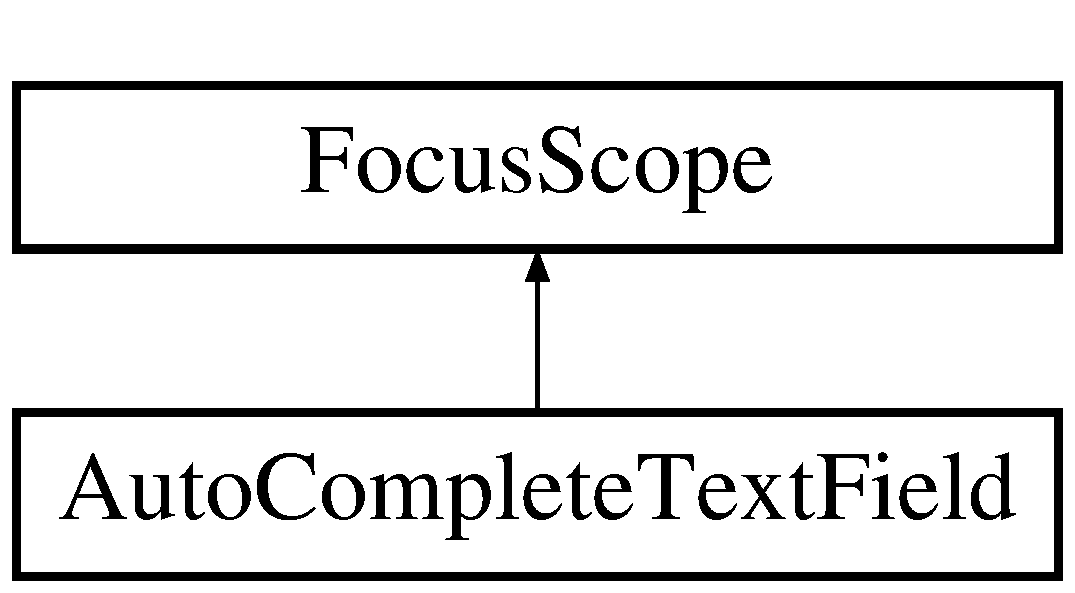
\includegraphics[height=2.000000cm]{classAutoCompleteTextField}
\end{center}
\end{figure}
\subsection*{Signals}
\begin{DoxyCompactItemize}
\item 
void \hyperlink{classAutoCompleteTextField_ac25877666f204e1262f089964c433868}{return\-Pressed} (var event)
\end{DoxyCompactItemize}
\subsection*{Public Member Functions}
\begin{DoxyCompactItemize}
\item 
\hypertarget{classAutoCompleteTextField_a5b1d8d7c0aec58bcaa9f556493d8dbda}{void \hyperlink{classAutoCompleteTextField_a5b1d8d7c0aec58bcaa9f556493d8dbda}{accept\-Current\-Completion} ()}\label{classAutoCompleteTextField_a5b1d8d7c0aec58bcaa9f556493d8dbda}

\begin{DoxyCompactList}\small\item\em Accepts the currently selected auto completion. \end{DoxyCompactList}\end{DoxyCompactItemize}
\subsection*{Properties}
\begin{DoxyCompactItemize}
\item 
\hypertarget{classAutoCompleteTextField_a633ed88c3f0b7217561c4dbd0c4ea021}{\hyperlink{classAutoCompleteModel}{Auto\-Complete\-Model} \hyperlink{classAutoCompleteTextField_a633ed88c3f0b7217561c4dbd0c4ea021}{complete\-Model}}\label{classAutoCompleteTextField_a633ed88c3f0b7217561c4dbd0c4ea021}

\begin{DoxyCompactList}\small\item\em Used to obtain possible completions. \end{DoxyCompactList}\item 
\hypertarget{classAutoCompleteTextField_a969420d165123d0897e14887bde2a988}{string \hyperlink{classAutoCompleteTextField_a969420d165123d0897e14887bde2a988}{text}}\label{classAutoCompleteTextField_a969420d165123d0897e14887bde2a988}

\begin{DoxyCompactList}\small\item\em the text field's text \end{DoxyCompactList}\item 
\hypertarget{classAutoCompleteTextField_ae017eba891574653d44853c70c5f288e}{string \hyperlink{classAutoCompleteTextField_ae017eba891574653d44853c70c5f288e}{alternative\-Text}}\label{classAutoCompleteTextField_ae017eba891574653d44853c70c5f288e}

\begin{DoxyCompactList}\small\item\em shown if text is empty \end{DoxyCompactList}\item 
\hypertarget{classAutoCompleteTextField_aac0b683369ed7794810c7466149bea9f}{bool \hyperlink{classAutoCompleteTextField_aac0b683369ed7794810c7466149bea9f}{active\-Focus\-On\-Press}}\label{classAutoCompleteTextField_aac0b683369ed7794810c7466149bea9f}

\begin{DoxyCompactList}\small\item\em {\ttfamily true} if focus can be gained by clicking in the text field \end{DoxyCompactList}\item 
\hypertarget{classAutoCompleteTextField_a4b4a8370abd9f2c421de9e0316807ee8}{alias \hyperlink{classAutoCompleteTextField_a4b4a8370abd9f2c421de9e0316807ee8}{clip}}\label{classAutoCompleteTextField_a4b4a8370abd9f2c421de9e0316807ee8}

\begin{DoxyCompactList}\small\item\em type\-: bool use clipping to prevent long text being rendered outside the component \end{DoxyCompactList}\item 
bool \hyperlink{classAutoCompleteTextField_a710dfeff1a9fca62d3103dff06e06afb}{prefer\-Alternative\-Text}
\end{DoxyCompactItemize}


\subsection{Detailed Description}
A text field with autocompletion. 

Possible entries for autocompletion are shown in a list below the text field. 

\subsection{Member Function Documentation}
\hypertarget{classAutoCompleteTextField_ac25877666f204e1262f089964c433868}{\index{Auto\-Complete\-Text\-Field@{Auto\-Complete\-Text\-Field}!return\-Pressed@{return\-Pressed}}
\index{return\-Pressed@{return\-Pressed}!AutoCompleteTextField@{Auto\-Complete\-Text\-Field}}
\subsubsection[{return\-Pressed}]{\setlength{\rightskip}{0pt plus 5cm}void Auto\-Complete\-Text\-Field\-::return\-Pressed (
\begin{DoxyParamCaption}
\item[{var}]{event}
\end{DoxyParamCaption}
)\hspace{0.3cm}{\ttfamily [signal]}}}\label{classAutoCompleteTextField_ac25877666f204e1262f089964c433868}
Emitted when return is pressed while the text field has focus. 
\begin{DoxyParams}{Parameters}
{\em type} & Key\-Event the key event \\
\hline
\end{DoxyParams}


\subsection{Property Documentation}
\hypertarget{classAutoCompleteTextField_a710dfeff1a9fca62d3103dff06e06afb}{\index{Auto\-Complete\-Text\-Field@{Auto\-Complete\-Text\-Field}!prefer\-Alternative\-Text@{prefer\-Alternative\-Text}}
\index{prefer\-Alternative\-Text@{prefer\-Alternative\-Text}!AutoCompleteTextField@{Auto\-Complete\-Text\-Field}}
\subsubsection[{prefer\-Alternative\-Text}]{\setlength{\rightskip}{0pt plus 5cm}bool Auto\-Complete\-Text\-Field\-::prefer\-Alternative\-Text}}\label{classAutoCompleteTextField_a710dfeff1a9fca62d3103dff06e06afb}
true if the text field is hidden by default. The alternative text is shown instead. Gaining focus will show the text field. 

The documentation for this class was generated from the following file\-:\begin{DoxyCompactItemize}
\item 
/home/stoef/qt/projects/ddt/ddt/qml/ddt/Auto\-Complete\-Text\-Field.\-qml\end{DoxyCompactItemize}

\hypertarget{classBPSDebate}{\section{B\-P\-S\-Debate Class Reference}
\label{classBPSDebate}\index{B\-P\-S\-Debate@{B\-P\-S\-Debate}}
}


Represents a debate in B\-P\-S-\/format.  




{\ttfamily \#include $<$bpsdebate.\-h$>$}

Inheritance diagram for B\-P\-S\-Debate\-:\begin{figure}[H]
\begin{center}
\leavevmode
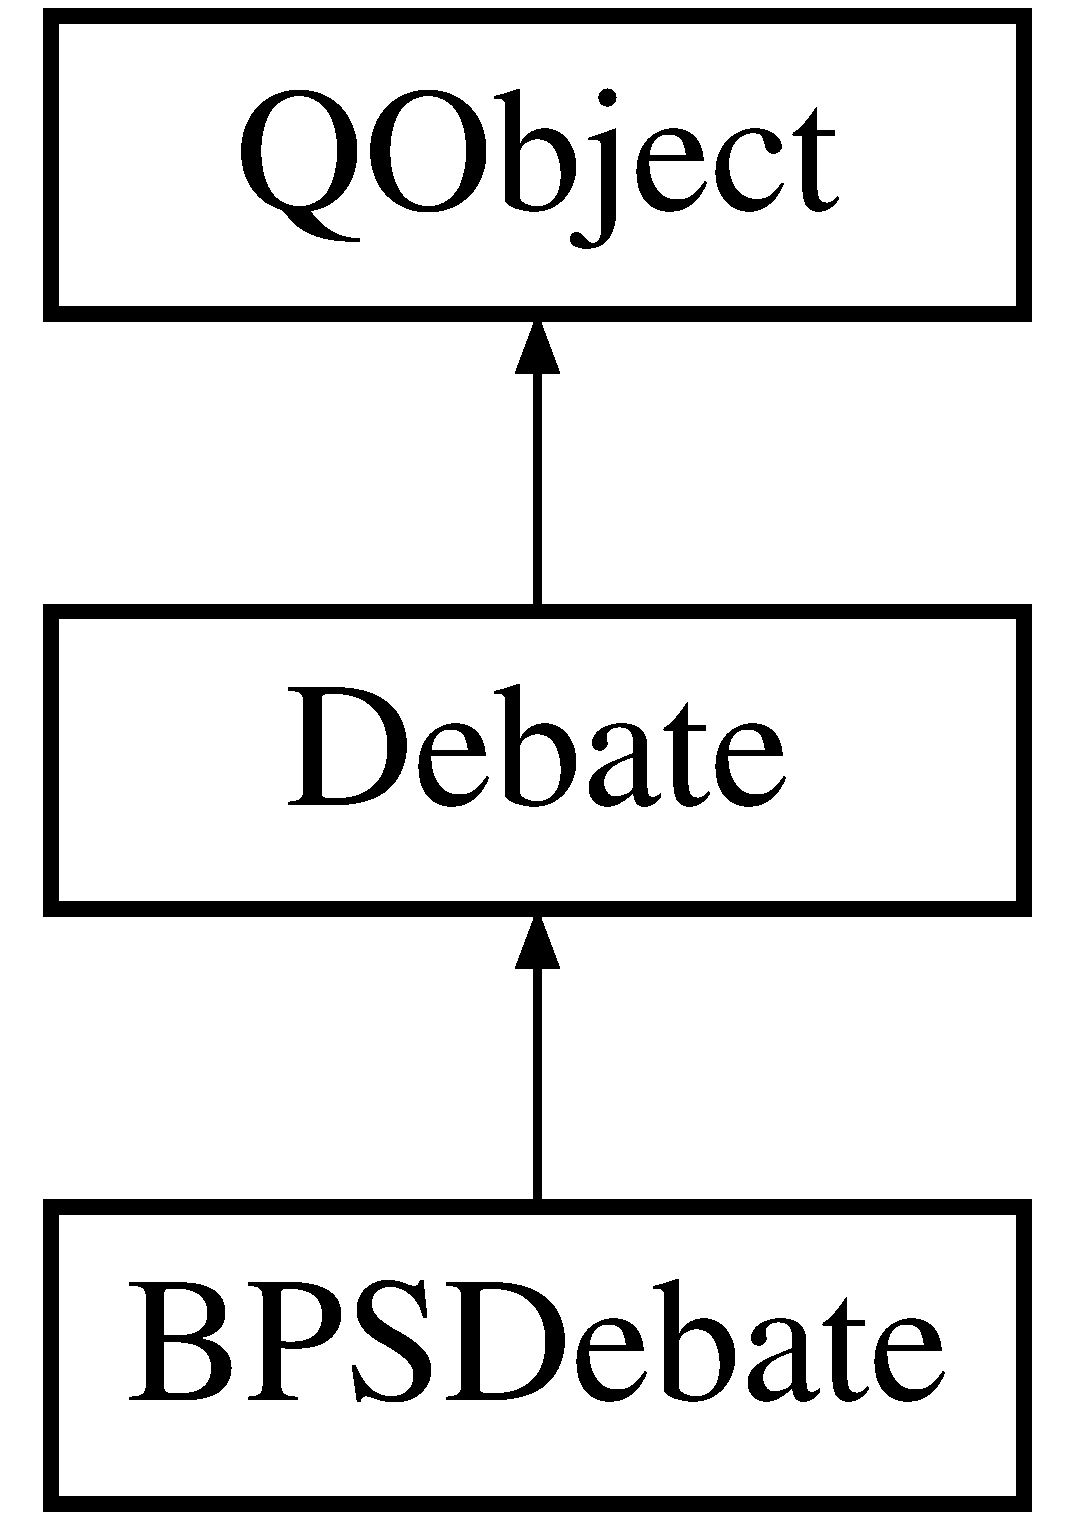
\includegraphics[height=3.000000cm]{classBPSDebate}
\end{center}
\end{figure}
\subsection*{Signals}
\begin{DoxyCompactItemize}
\item 
\hypertarget{classBPSDebate_acb0f8aa5921167908fd2fff0d2ffc809}{void {\bfseries gov1\-Places\-Changed} ()}\label{classBPSDebate_acb0f8aa5921167908fd2fff0d2ffc809}

\item 
\hypertarget{classBPSDebate_a95d0b266c9494ec0bd16030d78a54ea8}{void {\bfseries gov2\-Places\-Changed} ()}\label{classBPSDebate_a95d0b266c9494ec0bd16030d78a54ea8}

\item 
\hypertarget{classBPSDebate_aa88ab8369b13eab679458bf0efe38554}{void {\bfseries op1\-Places\-Changed} ()}\label{classBPSDebate_aa88ab8369b13eab679458bf0efe38554}

\item 
\hypertarget{classBPSDebate_aa71781723f82369b75f3af18cf50c5ba}{void {\bfseries op2\-Places\-Changed} ()}\label{classBPSDebate_aa71781723f82369b75f3af18cf50c5ba}

\end{DoxyCompactItemize}
\subsection*{Public Member Functions}
\begin{DoxyCompactItemize}
\item 
\hyperlink{classBPSDebate_aa8551c8847ba48d6020abdf2c6e0539d}{B\-P\-S\-Debate} (Q\-Object $\ast$parent=0)
\begin{DoxyCompactList}\small\item\em Creates a new B\-P\-S debate with default values. \end{DoxyCompactList}\item 
\hypertarget{classBPSDebate_a153f32f70c7ca8245a274794c0932a5f}{int {\bfseries gov1\-Places} ()}\label{classBPSDebate_a153f32f70c7ca8245a274794c0932a5f}

\item 
\hypertarget{classBPSDebate_a289e432b6dd9cee8f73e4a6d7a45f225}{void {\bfseries set\-Gov1\-Places} (int \hyperlink{classBPSDebate_aff0bc6617abe4eb69e9ddef87a0ad021}{gov1\-Places})}\label{classBPSDebate_a289e432b6dd9cee8f73e4a6d7a45f225}

\item 
\hypertarget{classBPSDebate_aab0e2510bd9492d2a0af01f01215eaec}{int {\bfseries gov2\-Places} ()}\label{classBPSDebate_aab0e2510bd9492d2a0af01f01215eaec}

\item 
\hypertarget{classBPSDebate_ae948a39ce6235568d30498a51ca68374}{void {\bfseries set\-Gov2\-Places} (int \hyperlink{classBPSDebate_adc50f853f398e82b65bb5013cc8f6ccc}{gov2\-Places})}\label{classBPSDebate_ae948a39ce6235568d30498a51ca68374}

\item 
\hypertarget{classBPSDebate_a20483fad2f39e2c5cdc0b6dc934334e3}{int {\bfseries op1\-Places} ()}\label{classBPSDebate_a20483fad2f39e2c5cdc0b6dc934334e3}

\item 
\hypertarget{classBPSDebate_a3f8642ce77566f4b452dbfae90568658}{void {\bfseries set\-Op1\-Places} (int \hyperlink{classBPSDebate_a299bc40d5f80b2d4066c7869f56c70ba}{op1\-Places})}\label{classBPSDebate_a3f8642ce77566f4b452dbfae90568658}

\item 
\hypertarget{classBPSDebate_a1a66edf202ff6181e0b26d1e0bcf8003}{int {\bfseries op2\-Places} ()}\label{classBPSDebate_a1a66edf202ff6181e0b26d1e0bcf8003}

\item 
\hypertarget{classBPSDebate_a59385753ceddc0899f1fad730aaadbc1}{void {\bfseries set\-Op2\-Places} (int \hyperlink{classBPSDebate_a98039d27d11878e68c88d41570553eae}{op2\-Places})}\label{classBPSDebate_a59385753ceddc0899f1fad730aaadbc1}

\item 
\hypertarget{classBPSDebate_a44c883b01ab5357a4fd07db2b7ff4dbc}{const Q\-List$<$ \hyperlink{classDebate_ae9871a36a2f3de7a7da8922d70fbece4}{Role\-Group} $>$ $\ast$ \hyperlink{classBPSDebate_a44c883b01ab5357a4fd07db2b7ff4dbc}{get\-Roles\-For\-Debate} ()}\label{classBPSDebate_a44c883b01ab5357a4fd07db2b7ff4dbc}

\begin{DoxyCompactList}\small\item\em Returns all roles that belong to this debate. \end{DoxyCompactList}\item 
\hypertarget{classBPSDebate_ab8f49170df500405e81e70ab83c4f70d}{\hyperlink{classDebate_a537fac343de1edd412012e4180b52e04}{Debate\-Format} {\bfseries format} ()}\label{classBPSDebate_ab8f49170df500405e81e70ab83c4f70d}

\item 
\hypertarget{classBPSDebate_a2674e7ed45e67a443fd36ca4b2d3a2a4}{int {\bfseries num\-Places} ()}\label{classBPSDebate_a2674e7ed45e67a443fd36ca4b2d3a2a4}

\end{DoxyCompactItemize}
\subsection*{Properties}
\begin{DoxyCompactItemize}
\item 
\hypertarget{classBPSDebate_aff0bc6617abe4eb69e9ddef87a0ad021}{int \hyperlink{classBPSDebate_aff0bc6617abe4eb69e9ddef87a0ad021}{gov1\-Places}}\label{classBPSDebate_aff0bc6617abe4eb69e9ddef87a0ad021}

\begin{DoxyCompactList}\small\item\em Holds the number of speakers in the first government. The default value is 2. \end{DoxyCompactList}\item 
\hypertarget{classBPSDebate_adc50f853f398e82b65bb5013cc8f6ccc}{int \hyperlink{classBPSDebate_adc50f853f398e82b65bb5013cc8f6ccc}{gov2\-Places}}\label{classBPSDebate_adc50f853f398e82b65bb5013cc8f6ccc}

\begin{DoxyCompactList}\small\item\em Holds the number of speakers in the second government. The default value is 2. \end{DoxyCompactList}\item 
\hypertarget{classBPSDebate_a299bc40d5f80b2d4066c7869f56c70ba}{int \hyperlink{classBPSDebate_a299bc40d5f80b2d4066c7869f56c70ba}{op1\-Places}}\label{classBPSDebate_a299bc40d5f80b2d4066c7869f56c70ba}

\begin{DoxyCompactList}\small\item\em Holds the number of speakers in the first opposition. The default value is 2. \end{DoxyCompactList}\item 
\hypertarget{classBPSDebate_a98039d27d11878e68c88d41570553eae}{int \hyperlink{classBPSDebate_a98039d27d11878e68c88d41570553eae}{op2\-Places}}\label{classBPSDebate_a98039d27d11878e68c88d41570553eae}

\begin{DoxyCompactList}\small\item\em Holds the number of speakers in the second opposition. The default value is 2. \end{DoxyCompactList}\end{DoxyCompactItemize}
\subsection*{Additional Inherited Members}


\subsection{Detailed Description}
Represents a debate in B\-P\-S-\/format. 

B\-P\-S (British Parliamentary Style) is a popular, internationally used format for debating. The debate has four different speaker roles, the first and second government and the first and second opposition. Each role consists of two speakers. The debate is judicated by at least one judicator.

This class allows the representation of understaffed debates with less than two speakers in a speaker role or no judicator. \begin{DoxySeeAlso}{See Also}
\hyperlink{classDebate}{Debate} \hyperlink{classOPDebate}{O\-P\-Debate} 
\end{DoxySeeAlso}


\subsection{Constructor \& Destructor Documentation}
\hypertarget{classBPSDebate_aa8551c8847ba48d6020abdf2c6e0539d}{\index{B\-P\-S\-Debate@{B\-P\-S\-Debate}!B\-P\-S\-Debate@{B\-P\-S\-Debate}}
\index{B\-P\-S\-Debate@{B\-P\-S\-Debate}!BPSDebate@{B\-P\-S\-Debate}}
\subsubsection[{B\-P\-S\-Debate}]{\setlength{\rightskip}{0pt plus 5cm}B\-P\-S\-Debate\-::\-B\-P\-S\-Debate (
\begin{DoxyParamCaption}
\item[{Q\-Object $\ast$}]{parent = {\ttfamily 0}}
\end{DoxyParamCaption}
)\hspace{0.3cm}{\ttfamily [explicit]}}}\label{classBPSDebate_aa8551c8847ba48d6020abdf2c6e0539d}


Creates a new B\-P\-S debate with default values. 


\begin{DoxyParams}{Parameters}
{\em parent} & the {\ttfamily Q\-Object's} parent \\
\hline
\end{DoxyParams}


The documentation for this class was generated from the following files\-:\begin{DoxyCompactItemize}
\item 
/home/stoef/qt/projects/ddt/ddt/src/bpsdebate.\-h\item 
/home/stoef/qt/projects/ddt/ddt/src/bpsdebate.\-cpp\end{DoxyCompactItemize}

\hypertarget{classBPSDebateView}{\section{B\-P\-S\-Debate\-View Class Reference}
\label{classBPSDebateView}\index{B\-P\-S\-Debate\-View@{B\-P\-S\-Debate\-View}}
}


Displays a B\-P\-S debate.  


Inheritance diagram for B\-P\-S\-Debate\-View\-:\begin{figure}[H]
\begin{center}
\leavevmode
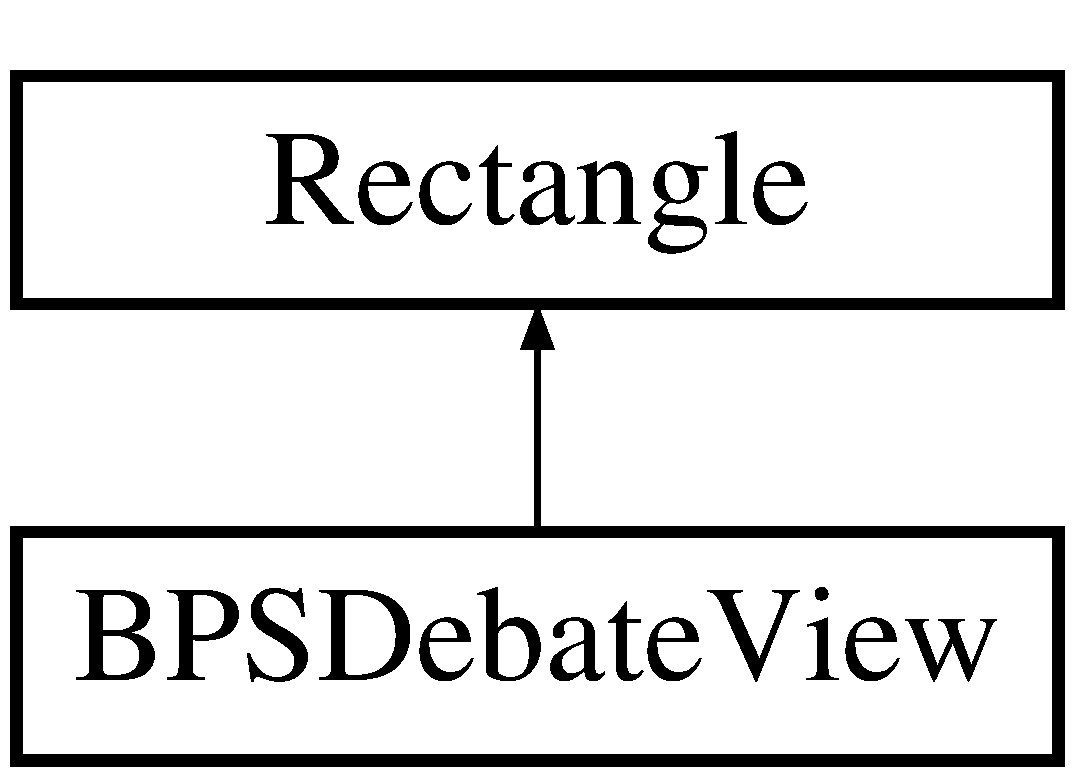
\includegraphics[height=2.000000cm]{classBPSDebateView}
\end{center}
\end{figure}
\subsection*{Signals}
\begin{DoxyCompactItemize}
\item 
\hypertarget{classBPSDebateView_af195c1b8ab918af612d86c74604f75cc}{void {\bfseries remove} ()}\label{classBPSDebateView_af195c1b8ab918af612d86c74604f75cc}

\end{DoxyCompactItemize}
\subsection*{Properties}
\begin{DoxyCompactItemize}
\item 
\hypertarget{classBPSDebateView_a2f4074285d7387aeb0fe55208d1f9b83}{\hyperlink{classBPSDebate}{B\-P\-S\-Debate} \hyperlink{classBPSDebateView_a2f4074285d7387aeb0fe55208d1f9b83}{bps\-Debate}}\label{classBPSDebateView_a2f4074285d7387aeb0fe55208d1f9b83}

\begin{DoxyCompactList}\small\item\em The debate that is displayed. \end{DoxyCompactList}\item 
\hypertarget{classBPSDebateView_a42784dfc74b99c528a9ee34357b27138}{bool \hyperlink{classBPSDebateView_a42784dfc74b99c528a9ee34357b27138}{editable}}\label{classBPSDebateView_a42784dfc74b99c528a9ee34357b27138}

\begin{DoxyCompactList}\small\item\em {\ttfamily true} if the room and the number of speakers should be editable. \end{DoxyCompactList}\item 
\hypertarget{classBPSDebateView_a10e5a3c749277df81a6ba90df18599b0}{\hyperlink{classSeatToSpeakerMapper}{Seat\-To\-Speaker\-Mapper} {\bfseries mapper}}\label{classBPSDebateView_a10e5a3c749277df81a6ba90df18599b0}

\end{DoxyCompactItemize}


\subsection{Detailed Description}
Displays a B\-P\-S debate. 

Allows editing the number of speakers participating in the debate. 

The documentation for this class was generated from the following file\-:\begin{DoxyCompactItemize}
\item 
/home/stoef/qt/projects/ddt/ddt/qml/ddt/B\-P\-S\-Debate\-View.\-qml\end{DoxyCompactItemize}

\hypertarget{classDDTConfiguration}{\section{D\-D\-T\-Configuration Class Reference}
\label{classDDTConfiguration}\index{D\-D\-T\-Configuration@{D\-D\-T\-Configuration}}
}


Reads options from a file.  




{\ttfamily \#include $<$ddtconfiguration.\-h$>$}

\subsection*{Public Member Functions}
\begin{DoxyCompactItemize}
\item 
\hyperlink{classDDTConfiguration_aa8b20f6bcfe2b3ddf61b96f2bab59cca}{D\-D\-T\-Configuration} (Q\-String file\-Name)
\begin{DoxyCompactList}\small\item\em \hyperlink{classDDTConfiguration}{D\-D\-T\-Configuration} Creates a new configuration object for a given configuration file. \end{DoxyCompactList}\item 
\hypertarget{classDDTConfiguration_a581c7466f9b308272470c1699601cf36}{void {\bfseries write\-Configuration\-File} (Q\-String file\-Name)}\label{classDDTConfiguration_a581c7466f9b308272470c1699601cf36}

\item 
Q\-Set$<$ Q\-String $>$ \hyperlink{classDDTConfiguration_a5124fbeb717acce377a1fbf8218b6d6d}{names} () const 
\begin{DoxyCompactList}\small\item\em Returns a list of names used for autocompletion. \end{DoxyCompactList}\item 
\hypertarget{classDDTConfiguration_ae74e28f9991535f8ff9af2c698c42cd4}{void \hyperlink{classDDTConfiguration_ae74e28f9991535f8ff9af2c698c42cd4}{add\-Name} (Q\-String name)}\label{classDDTConfiguration_ae74e28f9991535f8ff9af2c698c42cd4}

\begin{DoxyCompactList}\small\item\em add\-Name Adds a name to the list of known names used for autocompletion. \end{DoxyCompactList}\item 
Q\-String \hyperlink{classDDTConfiguration_aa6668d1848c30dccba2c2cfdbd9b7a5e}{language} () const 
\begin{DoxyCompactList}\small\item\em Returns the applications language (e.\-g. \char`\"{}en\char`\"{} or \char`\"{}de\char`\"{}) \end{DoxyCompactList}\item 
void \hyperlink{classDDTConfiguration_acc4051a3d29fedeaafcbfc6020962e3b}{set\-Language} (Q\-String \hyperlink{classDDTConfiguration_aa6668d1848c30dccba2c2cfdbd9b7a5e}{language})
\begin{DoxyCompactList}\small\item\em Sets the applications language that will be written in the configuration file. \end{DoxyCompactList}\end{DoxyCompactItemize}


\subsection{Detailed Description}
Reads options from a file. 

Reads generic configuration options from a given file, e.\-g. the applications language. The configuration is an xml-\/formatted document. Furthermore, writing or creating property files is supported. 

\subsection{Constructor \& Destructor Documentation}
\hypertarget{classDDTConfiguration_aa8b20f6bcfe2b3ddf61b96f2bab59cca}{\index{D\-D\-T\-Configuration@{D\-D\-T\-Configuration}!D\-D\-T\-Configuration@{D\-D\-T\-Configuration}}
\index{D\-D\-T\-Configuration@{D\-D\-T\-Configuration}!DDTConfiguration@{D\-D\-T\-Configuration}}
\subsubsection[{D\-D\-T\-Configuration}]{\setlength{\rightskip}{0pt plus 5cm}D\-D\-T\-Configuration\-::\-D\-D\-T\-Configuration (
\begin{DoxyParamCaption}
\item[{Q\-String}]{file\-Name}
\end{DoxyParamCaption}
)}}\label{classDDTConfiguration_aa8b20f6bcfe2b3ddf61b96f2bab59cca}


\hyperlink{classDDTConfiguration}{D\-D\-T\-Configuration} Creates a new configuration object for a given configuration file. 

A warning is given if the configuration file could not be loaded. In this case the class will return default values as properties 
\begin{DoxyParams}{Parameters}
{\em file\-Name} & the (relative) path to the configuration file. \\
\hline
\end{DoxyParams}


\subsection{Member Function Documentation}
\hypertarget{classDDTConfiguration_aa6668d1848c30dccba2c2cfdbd9b7a5e}{\index{D\-D\-T\-Configuration@{D\-D\-T\-Configuration}!language@{language}}
\index{language@{language}!DDTConfiguration@{D\-D\-T\-Configuration}}
\subsubsection[{language}]{\setlength{\rightskip}{0pt plus 5cm}Q\-String D\-D\-T\-Configuration\-::language (
\begin{DoxyParamCaption}
{}
\end{DoxyParamCaption}
) const\hspace{0.3cm}{\ttfamily [inline]}}}\label{classDDTConfiguration_aa6668d1848c30dccba2c2cfdbd9b7a5e}


Returns the applications language (e.\-g. \char`\"{}en\char`\"{} or \char`\"{}de\char`\"{}) 

An empty string is returned if the configuration file could not be loaded. \hypertarget{classDDTConfiguration_a5124fbeb717acce377a1fbf8218b6d6d}{\index{D\-D\-T\-Configuration@{D\-D\-T\-Configuration}!names@{names}}
\index{names@{names}!DDTConfiguration@{D\-D\-T\-Configuration}}
\subsubsection[{names}]{\setlength{\rightskip}{0pt plus 5cm}Q\-Set$<$Q\-String$>$ D\-D\-T\-Configuration\-::names (
\begin{DoxyParamCaption}
{}
\end{DoxyParamCaption}
) const\hspace{0.3cm}{\ttfamily [inline]}}}\label{classDDTConfiguration_a5124fbeb717acce377a1fbf8218b6d6d}


Returns a list of names used for autocompletion. 

An empty list is returned if the configuration file could not be loaded. \hypertarget{classDDTConfiguration_acc4051a3d29fedeaafcbfc6020962e3b}{\index{D\-D\-T\-Configuration@{D\-D\-T\-Configuration}!set\-Language@{set\-Language}}
\index{set\-Language@{set\-Language}!DDTConfiguration@{D\-D\-T\-Configuration}}
\subsubsection[{set\-Language}]{\setlength{\rightskip}{0pt plus 5cm}void D\-D\-T\-Configuration\-::set\-Language (
\begin{DoxyParamCaption}
\item[{Q\-String}]{language}
\end{DoxyParamCaption}
)\hspace{0.3cm}{\ttfamily [inline]}}}\label{classDDTConfiguration_acc4051a3d29fedeaafcbfc6020962e3b}


Sets the applications language that will be written in the configuration file. 


\begin{DoxyParams}{Parameters}
{\em language} & a country code \\
\hline
\end{DoxyParams}


The documentation for this class was generated from the following files\-:\begin{DoxyCompactItemize}
\item 
/home/stoef/qt/projects/ddt/ddt/src/ddtconfiguration.\-h\item 
/home/stoef/qt/projects/ddt/ddt/src/ddtconfiguration.\-cpp\end{DoxyCompactItemize}

\hypertarget{classDebate}{\section{Debate Class Reference}
\label{classDebate}\index{Debate@{Debate}}
}


Represents an abstract debate.  




{\ttfamily \#include $<$debate.\-h$>$}

Inheritance diagram for Debate\-:\begin{figure}[H]
\begin{center}
\leavevmode
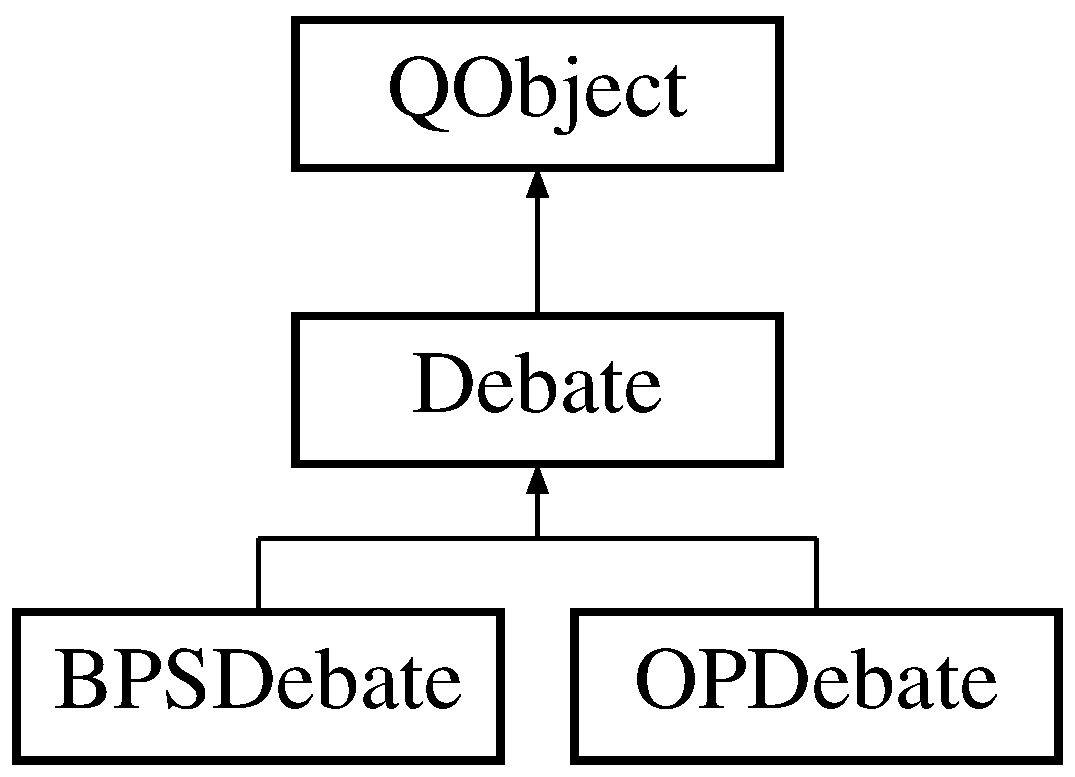
\includegraphics[height=3.000000cm]{classDebate}
\end{center}
\end{figure}
\subsection*{Public Types}
\begin{DoxyCompactItemize}
\item 
enum \hyperlink{classDebate_a537fac343de1edd412012e4180b52e04}{Debate\-Format} \{ \hyperlink{classDebate_a537fac343de1edd412012e4180b52e04a57900d539b2f8b08fba5e1df1622a3ad}{O\-P\-D}, 
\hyperlink{classDebate_a537fac343de1edd412012e4180b52e04afbefbbcc339cee2cb34f1be57d2168da}{B\-P\-S}
 \}
\begin{DoxyCompactList}\small\item\em Contains all supported debate formats. \end{DoxyCompactList}\item 
enum \hyperlink{classDebate_ae9871a36a2f3de7a7da8922d70fbece4}{Role\-Group} \{ \\*
\hyperlink{classDebate_ae9871a36a2f3de7a7da8922d70fbece4a51e2aa8f170ffbd3573aa117ca5f3eef}{J\-U\-D\-I\-C\-A\-T\-O\-R}, 
\hyperlink{classDebate_ae9871a36a2f3de7a7da8922d70fbece4a2556968b87c809f30b3e88ecf9a04180}{O\-P\-D\-\_\-\-G\-O\-V}, 
\hyperlink{classDebate_ae9871a36a2f3de7a7da8922d70fbece4a7232cd09530cdbdd6b3f460de7ff2746}{O\-P\-D\-\_\-\-O\-P}, 
\hyperlink{classDebate_ae9871a36a2f3de7a7da8922d70fbece4a9682891e23a589be8ffeeb19a907ae75}{O\-P\-D\-\_\-\-F\-F\-R}, 
\\*
\hyperlink{classDebate_ae9871a36a2f3de7a7da8922d70fbece4ae40d7e19be9a051ac4967d2bc815d851}{B\-P\-S\-\_\-\-G\-O\-V1}, 
\hyperlink{classDebate_ae9871a36a2f3de7a7da8922d70fbece4a519b0f35d90b536816035fa9fa1e52f7}{B\-P\-S\-\_\-\-G\-O\-V2}, 
\hyperlink{classDebate_ae9871a36a2f3de7a7da8922d70fbece4a950ec765be37e52b2b93e5cfc619048d}{B\-P\-S\-\_\-\-O\-P1}, 
\hyperlink{classDebate_ae9871a36a2f3de7a7da8922d70fbece4a09554f5050ad1a7de30cdfab1a4bb463}{B\-P\-S\-\_\-\-O\-P2}
 \}
\begin{DoxyCompactList}\small\item\em Contains all possible roles that speakers of a debate can have. \end{DoxyCompactList}\end{DoxyCompactItemize}
\subsection*{Signals}
\begin{DoxyCompactItemize}
\item 
\hypertarget{classDebate_a726099cea8180ac30a25ef2db7ff196e}{void {\bfseries room\-Changed} ()}\label{classDebate_a726099cea8180ac30a25ef2db7ff196e}

\item 
\hypertarget{classDebate_a66121202f07f259469f34339830bbb07}{void {\bfseries num\-Places\-Changed} ()}\label{classDebate_a66121202f07f259469f34339830bbb07}

\item 
\hypertarget{classDebate_a0901bfe451901b6d31ab5c7ecbef8d4a}{void {\bfseries judicator\-Places\-Changed} ()}\label{classDebate_a0901bfe451901b6d31ab5c7ecbef8d4a}

\end{DoxyCompactItemize}
\subsection*{Public Member Functions}
\begin{DoxyCompactItemize}
\item 
\hypertarget{classDebate_a89c49e04f0f5be4690ae6a0f231e2d57}{\hyperlink{classDebate_a89c49e04f0f5be4690ae6a0f231e2d57}{Debate} (Q\-Object $\ast$parent=0)}\label{classDebate_a89c49e04f0f5be4690ae6a0f231e2d57}

\begin{DoxyCompactList}\small\item\em Creates a new debate with a given parent. \end{DoxyCompactList}\item 
\hypertarget{classDebate_a6976d53aef96511860ee0610b35ef5d0}{Q\-String {\bfseries room} ()}\label{classDebate_a6976d53aef96511860ee0610b35ef5d0}

\item 
\hypertarget{classDebate_ad4d918691e512ca0e9f8bdfde1b60a7d}{void {\bfseries set\-Room} (Q\-String \hyperlink{classDebate_acab8c12e87212bbc6f14ce180bbdeccb}{room})}\label{classDebate_ad4d918691e512ca0e9f8bdfde1b60a7d}

\item 
\hypertarget{classDebate_a08898c144700ac4bfdf8176e79714c7c}{int {\bfseries judicator\-Places} ()}\label{classDebate_a08898c144700ac4bfdf8176e79714c7c}

\item 
\hypertarget{classDebate_a3a21fd3392281d2f1be94b8978c30e98}{void {\bfseries set\-Judicator\-Places} (int \hyperlink{classDebate_a871a42bb78323df624bd51ee733d3f5d}{judicator\-Places})}\label{classDebate_a3a21fd3392281d2f1be94b8978c30e98}

\item 
\hypertarget{classDebate_af280a91845695a6ad94e0a6bf6972a84}{virtual \hyperlink{classDebate_a537fac343de1edd412012e4180b52e04}{Debate\-Format} {\bfseries format} ()=0}\label{classDebate_af280a91845695a6ad94e0a6bf6972a84}

\item 
\hypertarget{classDebate_a52d7e3651ac81f31e3439a824b862f29}{virtual int {\bfseries num\-Places} ()}\label{classDebate_a52d7e3651ac81f31e3439a824b862f29}

\item 
\hypertarget{classDebate_ad4c84895868fd2e55e8d98c81afae7c6}{virtual const Q\-List$<$ \hyperlink{classDebate_ae9871a36a2f3de7a7da8922d70fbece4}{Role\-Group} $>$ $\ast$ \hyperlink{classDebate_ad4c84895868fd2e55e8d98c81afae7c6}{get\-Roles\-For\-Debate} ()=0}\label{classDebate_ad4c84895868fd2e55e8d98c81afae7c6}

\begin{DoxyCompactList}\small\item\em Returns all roles that belong to this debate. \end{DoxyCompactList}\end{DoxyCompactItemize}
\subsection*{Properties}
\begin{DoxyCompactItemize}
\item 
\hypertarget{classDebate_a871a42bb78323df624bd51ee733d3f5d}{int \hyperlink{classDebate_a871a42bb78323df624bd51ee733d3f5d}{judicator\-Places}}\label{classDebate_a871a42bb78323df624bd51ee733d3f5d}

\begin{DoxyCompactList}\small\item\em Holds the number of judicators used in this debates. Defaults to 1. \end{DoxyCompactList}\item 
\hypertarget{classDebate_acad1ad74183da0c383be84c62125efc4}{\hyperlink{classDebate_a537fac343de1edd412012e4180b52e04}{Debate\-Format} \hyperlink{classDebate_acad1ad74183da0c383be84c62125efc4}{format}}\label{classDebate_acad1ad74183da0c383be84c62125efc4}

\begin{DoxyCompactList}\small\item\em Holds the debates format. \end{DoxyCompactList}\item 
\hypertarget{classDebate_acab8c12e87212bbc6f14ce180bbdeccb}{Q\-String \hyperlink{classDebate_acab8c12e87212bbc6f14ce180bbdeccb}{room}}\label{classDebate_acab8c12e87212bbc6f14ce180bbdeccb}

\begin{DoxyCompactList}\small\item\em Holds the debates room. The room can be in arbitrary string. \end{DoxyCompactList}\item 
\hypertarget{classDebate_ad61df7c5685157f80dfb46c6efce4bce}{int \hyperlink{classDebate_ad61df7c5685157f80dfb46c6efce4bce}{num\-Places}}\label{classDebate_ad61df7c5685157f80dfb46c6efce4bce}

\begin{DoxyCompactList}\small\item\em Holds the complete number of places within this debate. \end{DoxyCompactList}\end{DoxyCompactItemize}


\subsection{Detailed Description}
Represents an abstract debate. 

This class serves as a superclass for all different debate formats. \begin{DoxySeeAlso}{See Also}
\hyperlink{classOPDebate}{O\-P\-Debate} \hyperlink{classBPSDebate}{B\-P\-S\-Debate} 
\end{DoxySeeAlso}


\subsection{Member Enumeration Documentation}
\hypertarget{classDebate_a537fac343de1edd412012e4180b52e04}{\index{Debate@{Debate}!Debate\-Format@{Debate\-Format}}
\index{Debate\-Format@{Debate\-Format}!Debate@{Debate}}
\subsubsection[{Debate\-Format}]{\setlength{\rightskip}{0pt plus 5cm}enum {\bf Debate\-::\-Debate\-Format}}}\label{classDebate_a537fac343de1edd412012e4180b52e04}


Contains all supported debate formats. 

\begin{Desc}
\item[Enumerator]\par
\begin{description}
\index{O\-P\-D@{O\-P\-D}!Debate@{Debate}}\index{Debate@{Debate}!O\-P\-D@{O\-P\-D}}\item[{\em 
\hypertarget{classDebate_a537fac343de1edd412012e4180b52e04a57900d539b2f8b08fba5e1df1622a3ad}{O\-P\-D}\label{classDebate_a537fac343de1edd412012e4180b52e04a57900d539b2f8b08fba5e1df1622a3ad}
}]Offene Parlamentarische Debatte, see \hyperlink{classOPDebate}{O\-P\-Debate} \index{B\-P\-S@{B\-P\-S}!Debate@{Debate}}\index{Debate@{Debate}!B\-P\-S@{B\-P\-S}}\item[{\em 
\hypertarget{classDebate_a537fac343de1edd412012e4180b52e04afbefbbcc339cee2cb34f1be57d2168da}{B\-P\-S}\label{classDebate_a537fac343de1edd412012e4180b52e04afbefbbcc339cee2cb34f1be57d2168da}
}]British Parliamentary Style debate, see \hyperlink{classBPSDebate}{B\-P\-S\-Debate} \end{description}
\end{Desc}
\hypertarget{classDebate_ae9871a36a2f3de7a7da8922d70fbece4}{\index{Debate@{Debate}!Role\-Group@{Role\-Group}}
\index{Role\-Group@{Role\-Group}!Debate@{Debate}}
\subsubsection[{Role\-Group}]{\setlength{\rightskip}{0pt plus 5cm}enum {\bf Debate\-::\-Role\-Group}}}\label{classDebate_ae9871a36a2f3de7a7da8922d70fbece4}


Contains all possible roles that speakers of a debate can have. 

\begin{Desc}
\item[Enumerator]\par
\begin{description}
\index{J\-U\-D\-I\-C\-A\-T\-O\-R@{J\-U\-D\-I\-C\-A\-T\-O\-R}!Debate@{Debate}}\index{Debate@{Debate}!J\-U\-D\-I\-C\-A\-T\-O\-R@{J\-U\-D\-I\-C\-A\-T\-O\-R}}\item[{\em 
\hypertarget{classDebate_ae9871a36a2f3de7a7da8922d70fbece4a51e2aa8f170ffbd3573aa117ca5f3eef}{J\-U\-D\-I\-C\-A\-T\-O\-R}\label{classDebate_ae9871a36a2f3de7a7da8922d70fbece4a51e2aa8f170ffbd3573aa117ca5f3eef}
}]The judicator role \index{O\-P\-D\-\_\-\-G\-O\-V@{O\-P\-D\-\_\-\-G\-O\-V}!Debate@{Debate}}\index{Debate@{Debate}!O\-P\-D\-\_\-\-G\-O\-V@{O\-P\-D\-\_\-\-G\-O\-V}}\item[{\em 
\hypertarget{classDebate_ae9871a36a2f3de7a7da8922d70fbece4a2556968b87c809f30b3e88ecf9a04180}{O\-P\-D\-\_\-\-G\-O\-V}\label{classDebate_ae9871a36a2f3de7a7da8922d70fbece4a2556968b87c809f30b3e88ecf9a04180}
}]The government role of O\-P\-D \index{O\-P\-D\-\_\-\-O\-P@{O\-P\-D\-\_\-\-O\-P}!Debate@{Debate}}\index{Debate@{Debate}!O\-P\-D\-\_\-\-O\-P@{O\-P\-D\-\_\-\-O\-P}}\item[{\em 
\hypertarget{classDebate_ae9871a36a2f3de7a7da8922d70fbece4a7232cd09530cdbdd6b3f460de7ff2746}{O\-P\-D\-\_\-\-O\-P}\label{classDebate_ae9871a36a2f3de7a7da8922d70fbece4a7232cd09530cdbdd6b3f460de7ff2746}
}]The opposition role of O\-P\-D \index{O\-P\-D\-\_\-\-F\-F\-R@{O\-P\-D\-\_\-\-F\-F\-R}!Debate@{Debate}}\index{Debate@{Debate}!O\-P\-D\-\_\-\-F\-F\-R@{O\-P\-D\-\_\-\-F\-F\-R}}\item[{\em 
\hypertarget{classDebate_ae9871a36a2f3de7a7da8922d70fbece4a9682891e23a589be8ffeeb19a907ae75}{O\-P\-D\-\_\-\-F\-F\-R}\label{classDebate_ae9871a36a2f3de7a7da8922d70fbece4a9682891e23a589be8ffeeb19a907ae75}
}]The F\-F\-R role of O\-P\-D \index{B\-P\-S\-\_\-\-G\-O\-V1@{B\-P\-S\-\_\-\-G\-O\-V1}!Debate@{Debate}}\index{Debate@{Debate}!B\-P\-S\-\_\-\-G\-O\-V1@{B\-P\-S\-\_\-\-G\-O\-V1}}\item[{\em 
\hypertarget{classDebate_ae9871a36a2f3de7a7da8922d70fbece4ae40d7e19be9a051ac4967d2bc815d851}{B\-P\-S\-\_\-\-G\-O\-V1}\label{classDebate_ae9871a36a2f3de7a7da8922d70fbece4ae40d7e19be9a051ac4967d2bc815d851}
}]The first government role of B\-P\-S \index{B\-P\-S\-\_\-\-G\-O\-V2@{B\-P\-S\-\_\-\-G\-O\-V2}!Debate@{Debate}}\index{Debate@{Debate}!B\-P\-S\-\_\-\-G\-O\-V2@{B\-P\-S\-\_\-\-G\-O\-V2}}\item[{\em 
\hypertarget{classDebate_ae9871a36a2f3de7a7da8922d70fbece4a519b0f35d90b536816035fa9fa1e52f7}{B\-P\-S\-\_\-\-G\-O\-V2}\label{classDebate_ae9871a36a2f3de7a7da8922d70fbece4a519b0f35d90b536816035fa9fa1e52f7}
}]The second government role of B\-P\-S \index{B\-P\-S\-\_\-\-O\-P1@{B\-P\-S\-\_\-\-O\-P1}!Debate@{Debate}}\index{Debate@{Debate}!B\-P\-S\-\_\-\-O\-P1@{B\-P\-S\-\_\-\-O\-P1}}\item[{\em 
\hypertarget{classDebate_ae9871a36a2f3de7a7da8922d70fbece4a950ec765be37e52b2b93e5cfc619048d}{B\-P\-S\-\_\-\-O\-P1}\label{classDebate_ae9871a36a2f3de7a7da8922d70fbece4a950ec765be37e52b2b93e5cfc619048d}
}]The first opposition role of B\-P\-S \index{B\-P\-S\-\_\-\-O\-P2@{B\-P\-S\-\_\-\-O\-P2}!Debate@{Debate}}\index{Debate@{Debate}!B\-P\-S\-\_\-\-O\-P2@{B\-P\-S\-\_\-\-O\-P2}}\item[{\em 
\hypertarget{classDebate_ae9871a36a2f3de7a7da8922d70fbece4a09554f5050ad1a7de30cdfab1a4bb463}{B\-P\-S\-\_\-\-O\-P2}\label{classDebate_ae9871a36a2f3de7a7da8922d70fbece4a09554f5050ad1a7de30cdfab1a4bb463}
}]The second opposition role of B\-P\-S \end{description}
\end{Desc}


The documentation for this class was generated from the following files\-:\begin{DoxyCompactItemize}
\item 
/home/stoef/qt/projects/ddt/ddt/src/debate.\-h\item 
/home/stoef/qt/projects/ddt/ddt/src/debate.\-cpp\end{DoxyCompactItemize}

\hypertarget{classDebatePage}{\section{Debate\-Page Class Reference}
\label{classDebatePage}\index{Debate\-Page@{Debate\-Page}}
}


Displays a component that allows editing the applications debate's.  


Inheritance diagram for Debate\-Page\-:\begin{figure}[H]
\begin{center}
\leavevmode
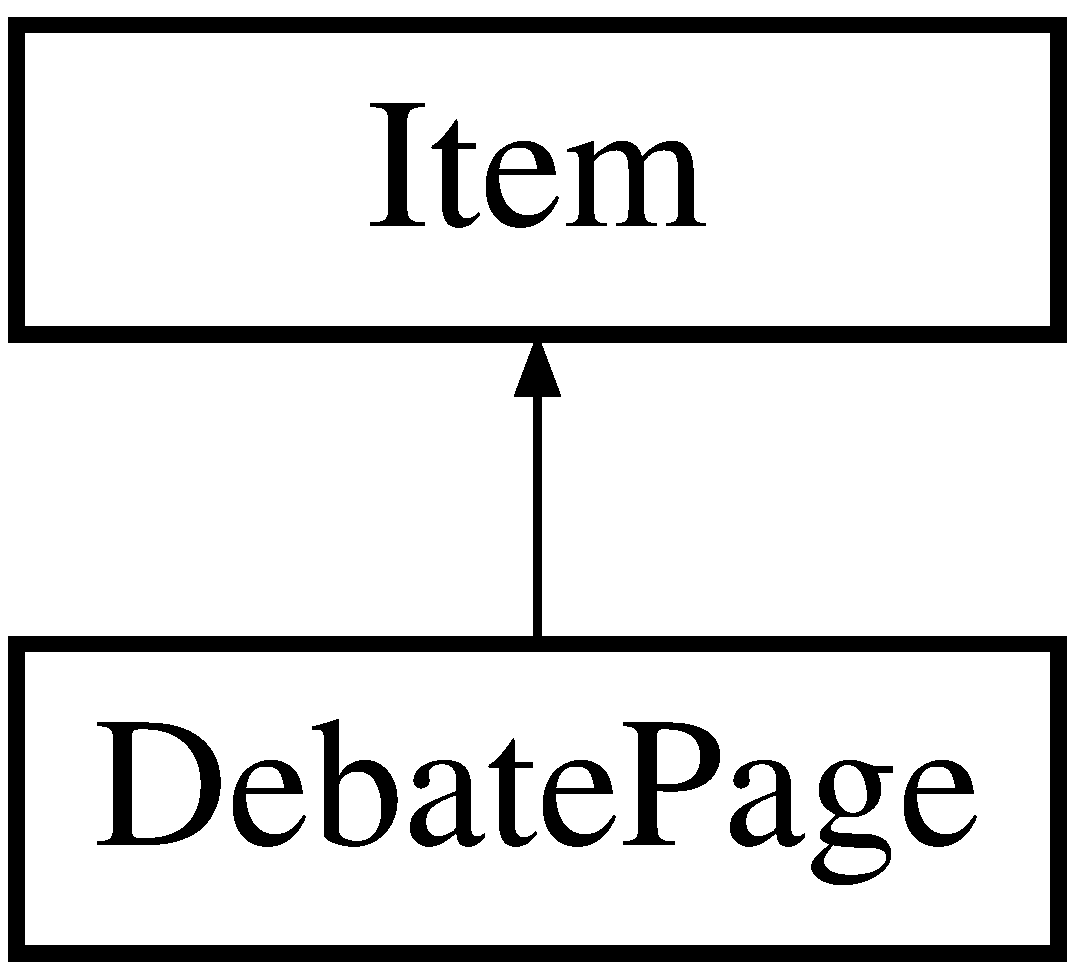
\includegraphics[height=2.000000cm]{classDebatePage}
\end{center}
\end{figure}
\subsection*{Properties}
\begin{DoxyCompactItemize}
\item 
\hypertarget{classDebatePage_a2591e3863cd1d80095d1c2a259bcf77b}{\hyperlink{classMainModel}{Main\-Model} \hyperlink{classDebatePage_a2591e3863cd1d80095d1c2a259bcf77b}{main\-Model}}\label{classDebatePage_a2591e3863cd1d80095d1c2a259bcf77b}

\begin{DoxyCompactList}\small\item\em The application's main\-Model. \end{DoxyCompactList}\item 
\hypertarget{classDebatePage_a6c33a9ff03852ccd00fd1a4b0ce88930}{Component \hyperlink{classDebatePage_a6c33a9ff03852ccd00fd1a4b0ce88930}{tool\-Bar\-Component}}\label{classDebatePage_a6c33a9ff03852ccd00fd1a4b0ce88930}

\begin{DoxyCompactList}\small\item\em A component with tool buttons that can be displayed in a tool bar. \end{DoxyCompactList}\item 
\hypertarget{classDebatePage_acbf69a0adb66d050aeea3f0e3b72c57d}{Action \hyperlink{classDebatePage_acbf69a0adb66d050aeea3f0e3b72c57d}{add\-Bps\-Debate\-Action}}\label{classDebatePage_acbf69a0adb66d050aeea3f0e3b72c57d}

\begin{DoxyCompactList}\small\item\em An action that should be used when adding a B\-P\-S debate. \end{DoxyCompactList}\item 
\hypertarget{classDebatePage_a9f0d42c01a1e321aaf9fb3af44b83d0b}{Action \hyperlink{classDebatePage_a9f0d42c01a1e321aaf9fb3af44b83d0b}{add\-Opd\-Action}}\label{classDebatePage_a9f0d42c01a1e321aaf9fb3af44b83d0b}

\begin{DoxyCompactList}\small\item\em An action that should be used when adding an O\-P\-D. \end{DoxyCompactList}\end{DoxyCompactItemize}


\subsection{Detailed Description}
Displays a component that allows editing the applications debate's. 

Allows adding and removing debates. The debates speaker counts and room names can be edited, too. 

The documentation for this class was generated from the following file\-:\begin{DoxyCompactItemize}
\item 
/home/stoef/qt/projects/ddt/ddt/qml/ddt/Debate\-Page.\-qml\end{DoxyCompactItemize}

\hypertarget{classFocusAndEditTextField}{\section{Focus\-And\-Edit\-Text\-Field Class Reference}
\label{classFocusAndEditTextField}\index{Focus\-And\-Edit\-Text\-Field@{Focus\-And\-Edit\-Text\-Field}}
}
Inheritance diagram for Focus\-And\-Edit\-Text\-Field\-:\begin{figure}[H]
\begin{center}
\leavevmode
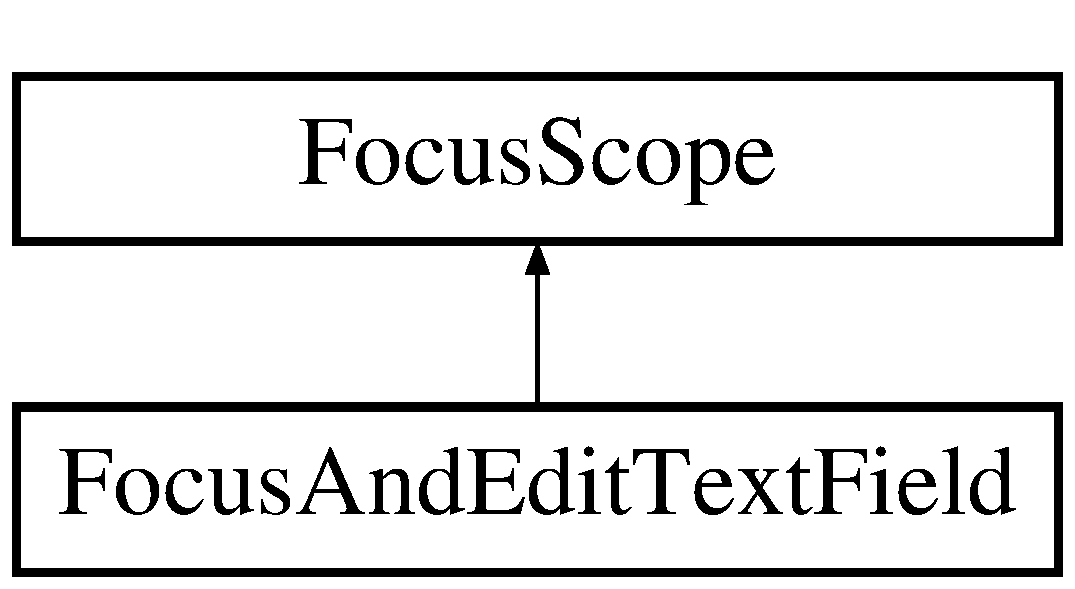
\includegraphics[height=2.000000cm]{classFocusAndEditTextField}
\end{center}
\end{figure}
\subsection*{Properties}
\begin{DoxyCompactItemize}
\item 
bool \hyperlink{classFocusAndEditTextField_af9099a4508112eccd7f6b0aea8cd3970}{editable}
\item 
\hypertarget{classFocusAndEditTextField_aeeed77be86ff52a0e1da7ce90b195511}{alias \hyperlink{classFocusAndEditTextField_aeeed77be86ff52a0e1da7ce90b195511}{text}}\label{classFocusAndEditTextField_aeeed77be86ff52a0e1da7ce90b195511}

\begin{DoxyCompactList}\small\item\em The text field's editable text. \end{DoxyCompactList}\item 
\hypertarget{classFocusAndEditTextField_a58220733c8bb84ab237df77f02b108c6}{alias \hyperlink{classFocusAndEditTextField_a58220733c8bb84ab237df77f02b108c6}{alternative\-Text}}\label{classFocusAndEditTextField_a58220733c8bb84ab237df77f02b108c6}

\begin{DoxyCompactList}\small\item\em The text field's alternative text, shown when not focussed. \end{DoxyCompactList}\item 
bool \hyperlink{classFocusAndEditTextField_ae40af8644ebd8001c47648f0934b0030}{prefer\-Alternative\-Text}
\item 
\hypertarget{classFocusAndEditTextField_a6ebf8b41df05ab797a3d62d521c102a5}{alias \hyperlink{classFocusAndEditTextField_a6ebf8b41df05ab797a3d62d521c102a5}{horizontal\-Alignment}}\label{classFocusAndEditTextField_a6ebf8b41df05ab797a3d62d521c102a5}

\begin{DoxyCompactList}\small\item\em The text field's horizontal aligmnent. \end{DoxyCompactList}\item 
\hypertarget{classFocusAndEditTextField_a7426f0bfdfdd1f6647b640f078bcc671}{alias {\bfseries font}}\label{classFocusAndEditTextField_a7426f0bfdfdd1f6647b640f078bcc671}

\end{DoxyCompactItemize}


\subsection{Detailed Description}
A text field with editing and display state, depending on focus.

This component holds a text field which displays its content differently depending on having focus or not. In editing mode, text is shown as a usual {\ttfamily Text\-Field}, in display mode, an alternative text is shown as an uneditable {\ttfamily Text} component. A single mouse click will attract focus and switch to editing state. 

\subsection{Property Documentation}
\hypertarget{classFocusAndEditTextField_af9099a4508112eccd7f6b0aea8cd3970}{\index{Focus\-And\-Edit\-Text\-Field@{Focus\-And\-Edit\-Text\-Field}!editable@{editable}}
\index{editable@{editable}!FocusAndEditTextField@{Focus\-And\-Edit\-Text\-Field}}
\subsubsection[{editable}]{\setlength{\rightskip}{0pt plus 5cm}bool Focus\-And\-Edit\-Text\-Field\-::editable}}\label{classFocusAndEditTextField_af9099a4508112eccd7f6b0aea8cd3970}
Holds if the text is editable. This component will act as a normal {\ttfamily Text} if set to {\ttfamily false}. \hypertarget{classFocusAndEditTextField_ae40af8644ebd8001c47648f0934b0030}{\index{Focus\-And\-Edit\-Text\-Field@{Focus\-And\-Edit\-Text\-Field}!prefer\-Alternative\-Text@{prefer\-Alternative\-Text}}
\index{prefer\-Alternative\-Text@{prefer\-Alternative\-Text}!FocusAndEditTextField@{Focus\-And\-Edit\-Text\-Field}}
\subsubsection[{prefer\-Alternative\-Text}]{\setlength{\rightskip}{0pt plus 5cm}bool Focus\-And\-Edit\-Text\-Field\-::prefer\-Alternative\-Text}}\label{classFocusAndEditTextField_ae40af8644ebd8001c47648f0934b0030}
The component will be shown as a normal text field, the alternative text is only shown when {\ttfamily text} is empty. 

The documentation for this class was generated from the following file\-:\begin{DoxyCompactItemize}
\item 
/home/stoef/qt/projects/ddt/ddt/qml/ddt/Focus\-And\-Edit\-Text\-Field.\-qml\end{DoxyCompactItemize}

\hypertarget{classHBar}{\section{H\-Bar Class Reference}
\label{classHBar}\index{H\-Bar@{H\-Bar}}
}


A simple gray horizontal bar, can be used to split different elements.  


Inheritance diagram for H\-Bar\-:\begin{figure}[H]
\begin{center}
\leavevmode
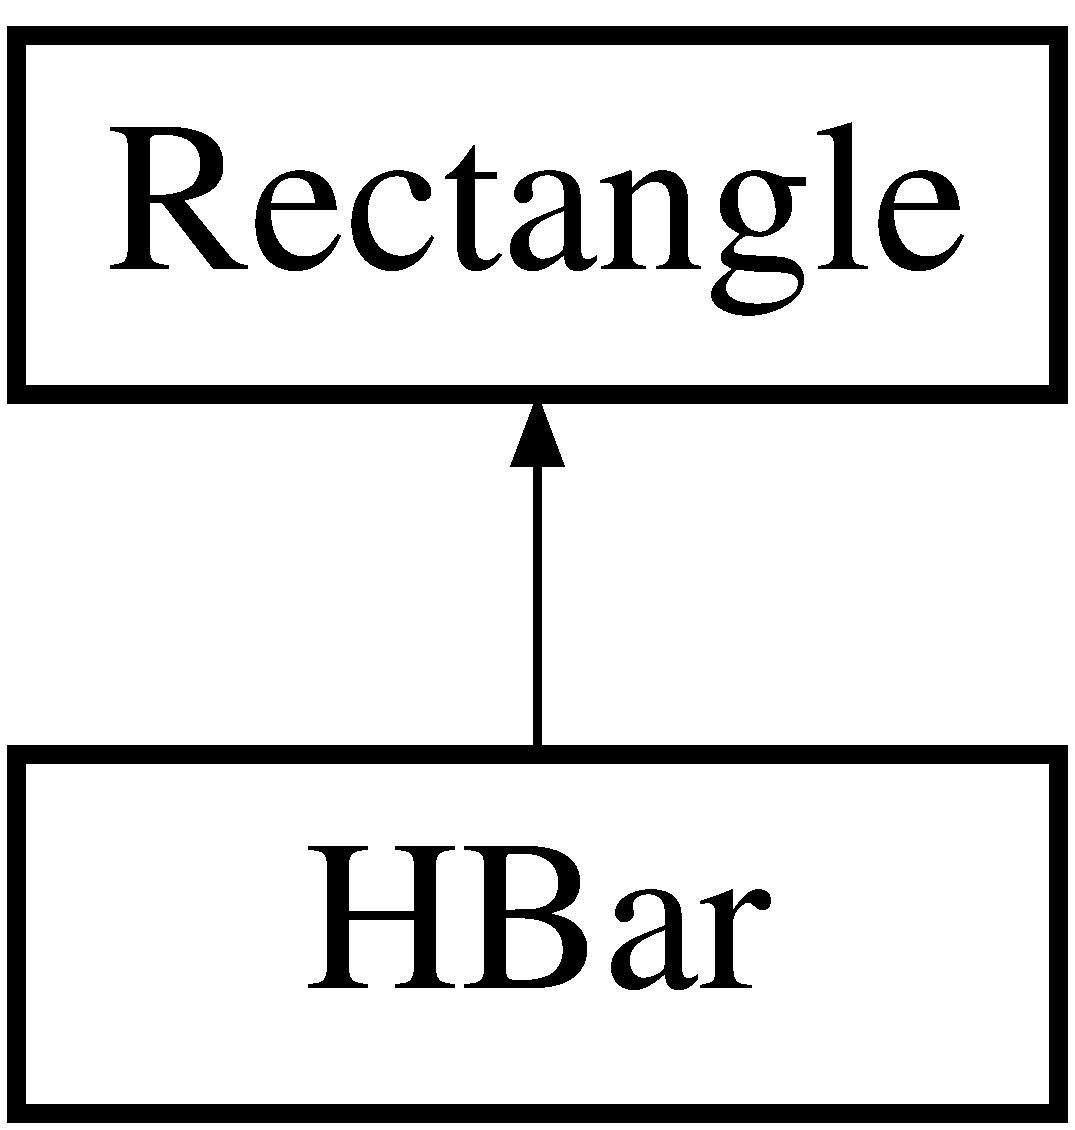
\includegraphics[height=2.000000cm]{classHBar}
\end{center}
\end{figure}


\subsection{Detailed Description}
A simple gray horizontal bar, can be used to split different elements. 

The documentation for this class was generated from the following file\-:\begin{DoxyCompactItemize}
\item 
/home/stoef/qt/projects/ddt/ddt/qml/ddt/H\-Bar.\-qml\end{DoxyCompactItemize}

\hypertarget{classInterruptHandler}{\section{Interrupt\-Handler Class Reference}
\label{classInterruptHandler}\index{Interrupt\-Handler@{Interrupt\-Handler}}
}
Inheritance diagram for Interrupt\-Handler\-:\begin{figure}[H]
\begin{center}
\leavevmode
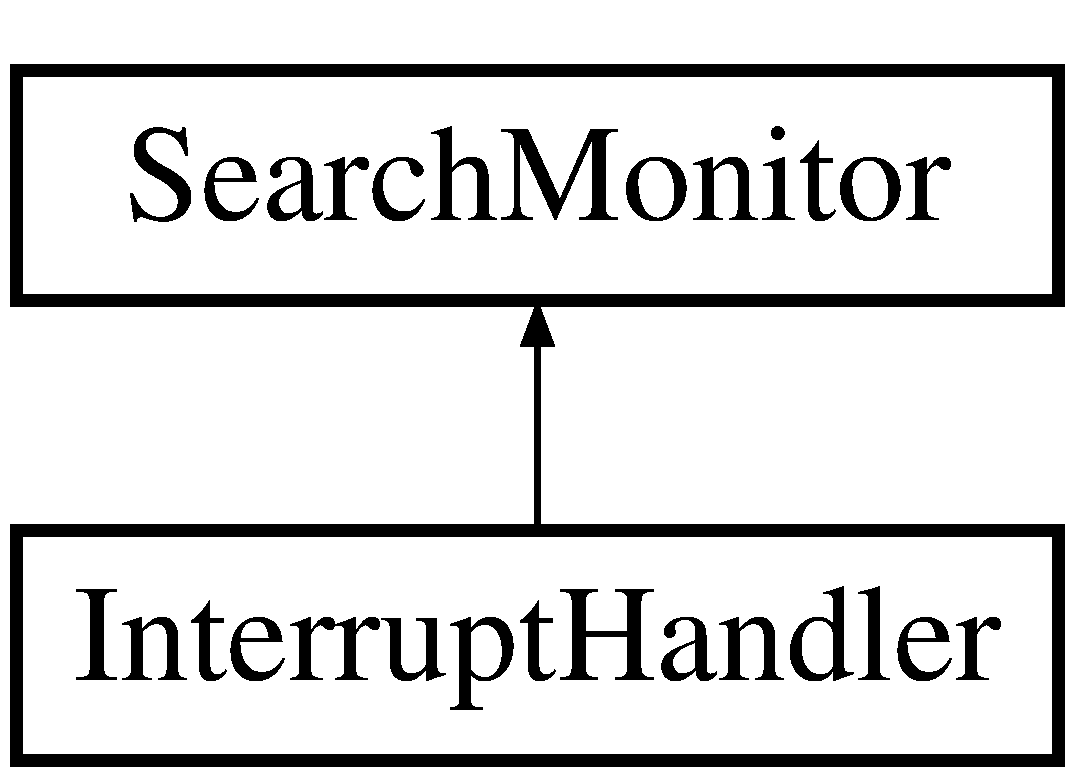
\includegraphics[height=2.000000cm]{classInterruptHandler}
\end{center}
\end{figure}
\subsection*{Public Member Functions}
\begin{DoxyCompactItemize}
\item 
\hypertarget{classInterruptHandler_a23d63a8baf03e339a76b0c81350e380d}{{\bfseries Interrupt\-Handler} (\hyperlink{classMatchingSolver}{Matching\-Solver} $\ast$ms, Solver $\ast$const s)}\label{classInterruptHandler_a23d63a8baf03e339a76b0c81350e380d}

\item 
\hypertarget{classInterruptHandler_a23f0af9de71fd7061d1fe3bc9ad55714}{void {\bfseries Begin\-Next\-Decision} (Decision\-Builder $\ast$const b)}\label{classInterruptHandler_a23f0af9de71fd7061d1fe3bc9ad55714}

\end{DoxyCompactItemize}


The documentation for this class was generated from the following file\-:\begin{DoxyCompactItemize}
\item 
/home/stoef/qt/projects/ddt/ddt/src/matchingsolver.\-cpp\end{DoxyCompactItemize}

\hypertarget{classmain}{\section{main Class Reference}
\label{classmain}\index{main@{main}}
}


D\-D\-T's one and only application window.  


Inheritance diagram for main\-:\begin{figure}[H]
\begin{center}
\leavevmode
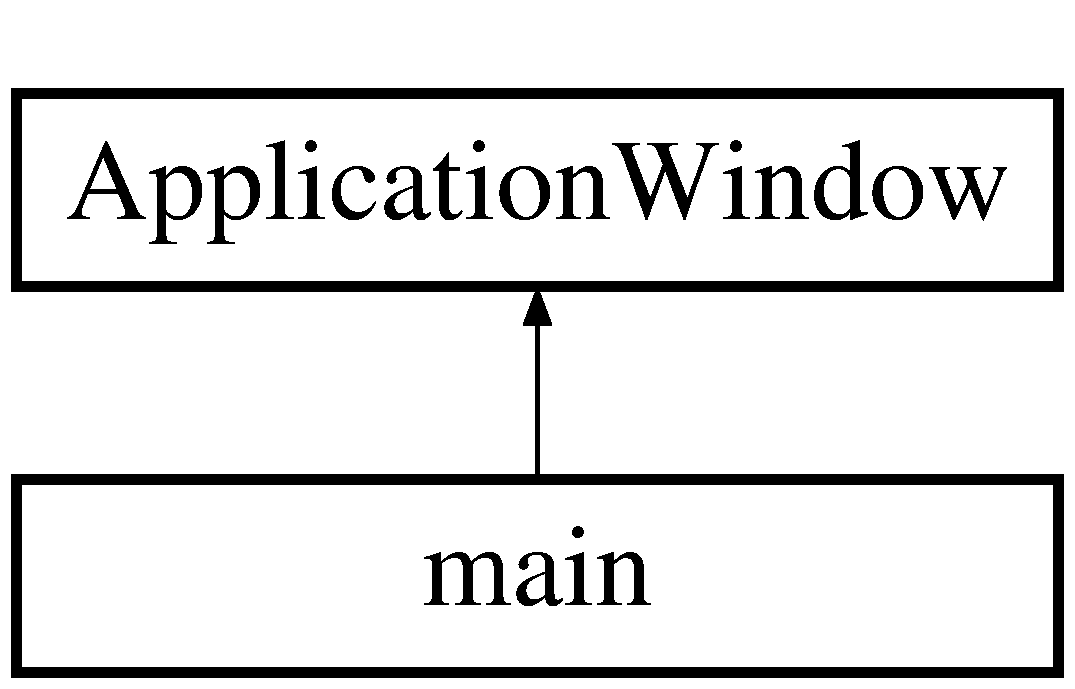
\includegraphics[height=2.000000cm]{classmain}
\end{center}
\end{figure}
\subsection*{Public Member Functions}
\begin{DoxyCompactItemize}
\item 
\hypertarget{classmain_a0c9e48faded0ac8427a982654422988b}{void {\bfseries restart\-Solver} ()}\label{classmain_a0c9e48faded0ac8427a982654422988b}

\item 
\hypertarget{classmain_a62b940da31d74ffbe7445af00bfd6a1f}{void \hyperlink{classmain_a62b940da31d74ffbe7445af00bfd6a1f}{change\-Language} (lang)}\label{classmain_a62b940da31d74ffbe7445af00bfd6a1f}

\begin{DoxyCompactList}\small\item\em Changes the application's language to a new value. Expects a country code as argument. \end{DoxyCompactList}\end{DoxyCompactItemize}
\subsection*{Properties}
\begin{DoxyCompactItemize}
\item 
int \hyperlink{classmain_a4ede4960616afa3a86ec26a159598ee6}{current\-Page}
\item 
\hypertarget{classmain_a2ec401feae2b853e39598efac50ecd00}{Q\-List\-Q\-M\-L\-Wrapper \hyperlink{classmain_a2ec401feae2b853e39598efac50ecd00}{selection\-Model}}\label{classmain_a2ec401feae2b853e39598efac50ecd00}

\begin{DoxyCompactList}\small\item\em Contains all currently selected speakers. \end{DoxyCompactList}\item 
\hypertarget{classmain_a25ba853e098b739e9ca20ac90d147bcf}{\hyperlink{classMainModel}{Main\-Model} \hyperlink{classmain_a25ba853e098b739e9ca20ac90d147bcf}{main\-Model}}\label{classmain_a25ba853e098b739e9ca20ac90d147bcf}

\begin{DoxyCompactList}\small\item\em Holds the applications main model. \end{DoxyCompactList}\item 
\hypertarget{classmain_a9a47f6e2e719fff4105c5d13f1bd21d5}{Action \hyperlink{classmain_a9a47f6e2e719fff4105c5d13f1bd21d5}{delete\-Selected\-Speakers}}\label{classmain_a9a47f6e2e719fff4105c5d13f1bd21d5}

\begin{DoxyCompactList}\small\item\em This action deletes all currently selected speakers. \end{DoxyCompactList}\item 
\hypertarget{classmain_ad70cac7cdc3f18247724cdf9cc0825c7}{Action \hyperlink{classmain_ad70cac7cdc3f18247724cdf9cc0825c7}{select\-All\-Action}}\label{classmain_ad70cac7cdc3f18247724cdf9cc0825c7}

\begin{DoxyCompactList}\small\item\em This action selects all available speakers. \end{DoxyCompactList}\item 
\hypertarget{classmain_a7c45ba5e198fc637bc4dd7a7651ac8b9}{Action \hyperlink{classmain_a7c45ba5e198fc637bc4dd7a7651ac8b9}{add\-Speaker\-Action}}\label{classmain_a7c45ba5e198fc637bc4dd7a7651ac8b9}

\begin{DoxyCompactList}\small\item\em Adds a new speaker with an empty name. \end{DoxyCompactList}\item 
\hypertarget{classmain_a74ad13024bcc95b34992303780e12d6d}{Action \hyperlink{classmain_a74ad13024bcc95b34992303780e12d6d}{add\-Bps\-Debate\-Action}}\label{classmain_a74ad13024bcc95b34992303780e12d6d}

\begin{DoxyCompactList}\small\item\em Adds a new B\-P\-S debate. \end{DoxyCompactList}\item 
\hypertarget{classmain_a750a0cdb3f5ce73ad765a9b0aa5ae92b}{Action \hyperlink{classmain_a750a0cdb3f5ce73ad765a9b0aa5ae92b}{add\-Opd\-Action}}\label{classmain_a750a0cdb3f5ce73ad765a9b0aa5ae92b}

\begin{DoxyCompactList}\small\item\em Adds a new O\-P debate. \end{DoxyCompactList}\item 
\hypertarget{classmain_a8a0e5e7da45ae92f3c70e8cb330a006f}{Action \hyperlink{classmain_a8a0e5e7da45ae92f3c70e8cb330a006f}{generate\-Solution\-Action}}\label{classmain_a8a0e5e7da45ae92f3c70e8cb330a006f}

\begin{DoxyCompactList}\small\item\em Generates a new solution. This will open the result page. \end{DoxyCompactList}\item 
\hypertarget{classmain_a4745a4fc2c425071adf6ffd45b8e859c}{Action \hyperlink{classmain_a4745a4fc2c425071adf6ffd45b8e859c}{interrupt\-Calculation\-Action}}\label{classmain_a4745a4fc2c425071adf6ffd45b8e859c}

\begin{DoxyCompactList}\small\item\em Interrupts the current calculation. \end{DoxyCompactList}\end{DoxyCompactItemize}


\subsection{Detailed Description}
D\-D\-T's one and only application window. 

\subsection{Property Documentation}
\hypertarget{classmain_a4ede4960616afa3a86ec26a159598ee6}{\index{main@{main}!current\-Page@{current\-Page}}
\index{current\-Page@{current\-Page}!main@{main}}
\subsubsection[{current\-Page}]{\setlength{\rightskip}{0pt plus 5cm}int main\-::current\-Page}}\label{classmain_a4ede4960616afa3a86ec26a159598ee6}
The currently selected page. 0 refers to the speaker page, 1 refers to the debate page, 2 refers to the solution page. 

The documentation for this class was generated from the following file\-:\begin{DoxyCompactItemize}
\item 
/home/stoef/qt/projects/ddt/ddt/qml/ddt/main.\-qml\end{DoxyCompactItemize}

\hypertarget{classMainModel}{\section{Main\-Model Class Reference}
\label{classMainModel}\index{Main\-Model@{Main\-Model}}
}


Offers access to all parts of the application's model.  




{\ttfamily \#include $<$mainmodel.\-h$>$}

Inheritance diagram for Main\-Model\-:\begin{figure}[H]
\begin{center}
\leavevmode
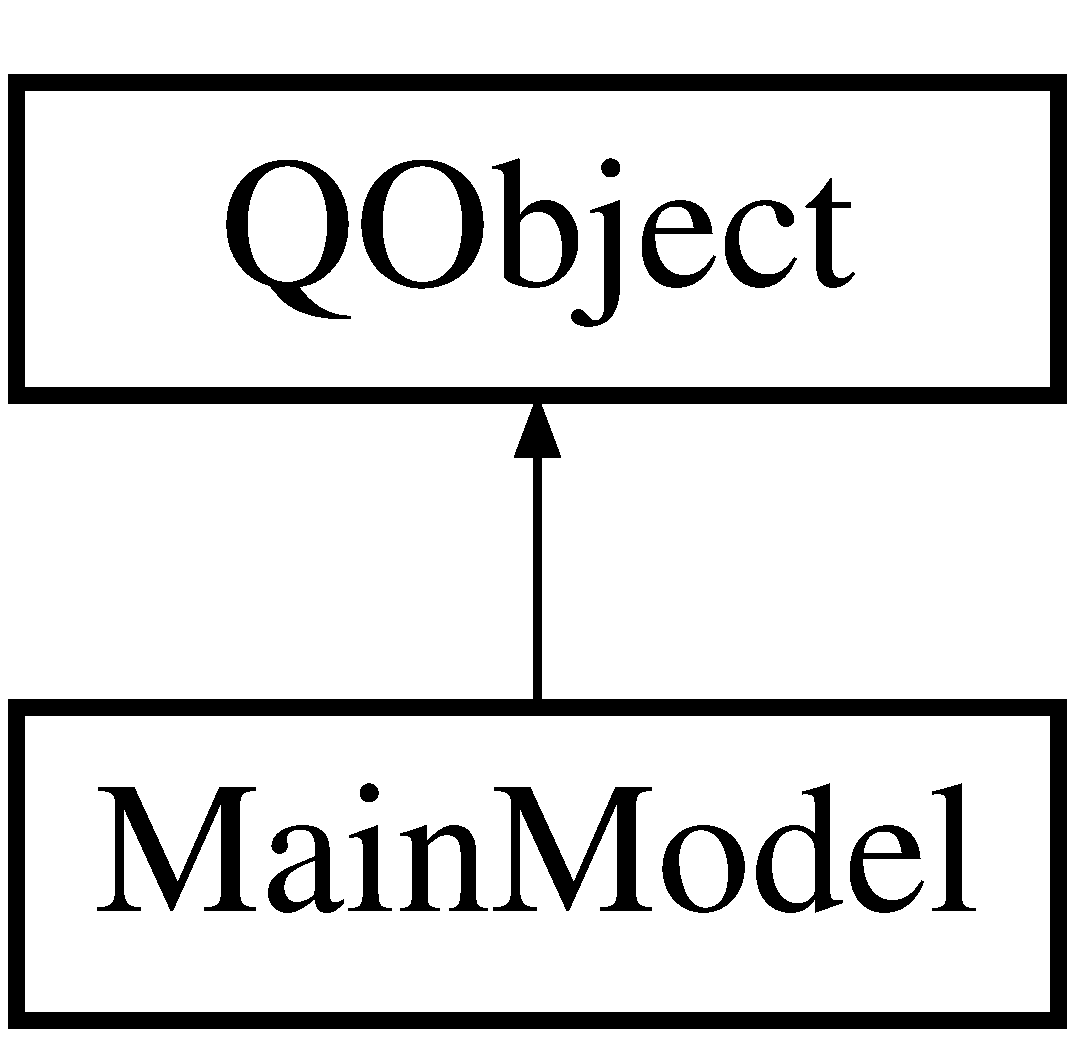
\includegraphics[height=2.000000cm]{classMainModel}
\end{center}
\end{figure}
\subsection*{Public Types}
\begin{DoxyCompactItemize}
\item 
enum \hyperlink{classMainModel_ab0047ea86efa2a40e9aff734f897c330}{Solution\-State} \{ \hyperlink{classMainModel_ab0047ea86efa2a40e9aff734f897c330ab53939240c4a4cba4af14afbd0a88acc}{U\-N\-K\-N\-O\-W\-N}, 
\hyperlink{classMainModel_ab0047ea86efa2a40e9aff734f897c330a380fb36b63f0bc9518789a36c785b027}{S\-O\-L\-U\-T\-I\-O\-N\-\_\-\-E\-X\-I\-S\-T\-S}, 
\hyperlink{classMainModel_ab0047ea86efa2a40e9aff734f897c330a10b96c9ee5c7b402033d5397b00be38d}{N\-O\-\_\-\-S\-O\-L\-U\-T\-I\-O\-N\-\_\-\-E\-X\-I\-S\-T\-S}, 
\hyperlink{classMainModel_ab0047ea86efa2a40e9aff734f897c330a7bc326ea163e937856ec2e520548e7f8}{C\-A\-L\-C\-U\-L\-A\-T\-I\-N\-G}
 \}
\begin{DoxyCompactList}\small\item\em Specifies the application's solution state. \end{DoxyCompactList}\end{DoxyCompactItemize}
\subsection*{Signals}
\begin{DoxyCompactItemize}
\item 
\hypertarget{classMainModel_a64cbb6676acd654918493189d3667ac8}{void {\bfseries solution\-Count\-Changed} ()}\label{classMainModel_a64cbb6676acd654918493189d3667ac8}

\item 
\hypertarget{classMainModel_a81d839de094a197583453b9c567eb8df}{void {\bfseries solution\-State\-Changed} ()}\label{classMainModel_a81d839de094a197583453b9c567eb8df}

\item 
\hypertarget{classMainModel_a77e0d8e44310724ffd717e6e5eb91b68}{void {\bfseries num\-Places\-Changed} ()}\label{classMainModel_a77e0d8e44310724ffd717e6e5eb91b68}

\end{DoxyCompactItemize}
\subsection*{Public Member Functions}
\begin{DoxyCompactItemize}
\item 
\hyperlink{classMainModel_a6c11a3942ed91eda77c4901d3d4f95b5}{Main\-Model} (Q\-String config\-File=\char`\"{}options.\-xml\char`\"{}, Q\-Object $\ast$parent=0)
\begin{DoxyCompactList}\small\item\em Constructs a new {\ttfamily \hyperlink{classMainModel}{Main\-Model}}. \end{DoxyCompactList}\item 
\hypertarget{classMainModel_af573c08c12cc35fb7a961b98a559d21b}{\hyperlink{classMainModel_af573c08c12cc35fb7a961b98a559d21b}{$\sim$\-Main\-Model} ()}\label{classMainModel_af573c08c12cc35fb7a961b98a559d21b}

\begin{DoxyCompactList}\small\item\em Deletes the main model and releases all ressources. \end{DoxyCompactList}\item 
\hypertarget{classMainModel_a07df104ce3e2f27de3f5f4a1abe554eb}{\hyperlink{classQListQmlWrapper}{Q\-List\-Qml\-Wrapper} $\ast$ {\bfseries debates} ()}\label{classMainModel_a07df104ce3e2f27de3f5f4a1abe554eb}

\item 
\hypertarget{classMainModel_a0ee2c2d98c9384a91e3a0eda721eb9c3}{\hyperlink{classQListQmlWrapper}{Q\-List\-Qml\-Wrapper} $\ast$ {\bfseries speaker\-List} ()}\label{classMainModel_a0ee2c2d98c9384a91e3a0eda721eb9c3}

\item 
\hypertarget{classMainModel_a27a5d15b68e83bb899e6208cc8dd1a18}{\hyperlink{classQListQmlWrapper}{Q\-List\-Qml\-Wrapper} $\ast$ {\bfseries teams} ()}\label{classMainModel_a27a5d15b68e83bb899e6208cc8dd1a18}

\item 
\hypertarget{classMainModel_a70a4770c8bae2da24bf447203da8f8c3}{\hyperlink{classAutoCompleteModel}{Auto\-Complete\-Model} $\ast$ {\bfseries auto\-Complete\-Model} ()}\label{classMainModel_a70a4770c8bae2da24bf447203da8f8c3}

\item 
Q\-\_\-\-I\-N\-V\-O\-K\-A\-B\-L\-E void \hyperlink{classMainModel_adf2889da5df77b5fc400d342b3f5ed41}{add\-Speaker} ()
\begin{DoxyCompactList}\small\item\em Same as. \end{DoxyCompactList}\item 
\hypertarget{classMainModel_a3383a2c9e268f9b2d0f132c1113d4ecd}{Q\-\_\-\-I\-N\-V\-O\-K\-A\-B\-L\-E void \hyperlink{classMainModel_a3383a2c9e268f9b2d0f132c1113d4ecd}{add\-Speaker} (Q\-String name)}\label{classMainModel_a3383a2c9e268f9b2d0f132c1113d4ecd}

\begin{DoxyCompactList}\small\item\em Creates a new speaker with a given name and adds him to the speaker list. \end{DoxyCompactList}\item 
\hypertarget{classMainModel_ad40184a652b1747e54fe292596988406}{Q\-\_\-\-I\-N\-V\-O\-K\-A\-B\-L\-E void \hyperlink{classMainModel_ad40184a652b1747e54fe292596988406}{remove\-Speaker} (int index)}\label{classMainModel_ad40184a652b1747e54fe292596988406}

\begin{DoxyCompactList}\small\item\em Removes a speaker at a given position in the speaker list. \end{DoxyCompactList}\item 
\hypertarget{classMainModel_aacae118923c35695011e123fd23fa953}{Q\-\_\-\-I\-N\-V\-O\-K\-A\-B\-L\-E void \hyperlink{classMainModel_aacae118923c35695011e123fd23fa953}{remove\-Speaker} (\hyperlink{classSpeakerModel}{Speaker\-Model} $\ast$speaker)}\label{classMainModel_aacae118923c35695011e123fd23fa953}

\begin{DoxyCompactList}\small\item\em Removes a given speaker. \end{DoxyCompactList}\item 
\hypertarget{classMainModel_a07cfd68a24326492b77f4e894c271ec1}{Q\-\_\-\-I\-N\-V\-O\-K\-A\-B\-L\-E void \hyperlink{classMainModel_a07cfd68a24326492b77f4e894c271ec1}{add\-Op\-Debate} ()}\label{classMainModel_a07cfd68a24326492b77f4e894c271ec1}

\begin{DoxyCompactList}\small\item\em Adds a new O\-P-\/\-Debate to the application's debate list. \end{DoxyCompactList}\item 
\hypertarget{classMainModel_a7ecaa63c19d9a441ec3256dfc3ded2de}{Q\-\_\-\-I\-N\-V\-O\-K\-A\-B\-L\-E void \hyperlink{classMainModel_a7ecaa63c19d9a441ec3256dfc3ded2de}{add\-Bps\-Debate} ()}\label{classMainModel_a7ecaa63c19d9a441ec3256dfc3ded2de}

\begin{DoxyCompactList}\small\item\em Adds a new B\-P\-S-\/\-Debate to the application's debate list. \end{DoxyCompactList}\item 
\hypertarget{classMainModel_ab7aee65aefd3d6bf4f19c4e306ed7efd}{Q\-\_\-\-I\-N\-V\-O\-K\-A\-B\-L\-E void \hyperlink{classMainModel_ab7aee65aefd3d6bf4f19c4e306ed7efd}{remove\-Debate} (int index)}\label{classMainModel_ab7aee65aefd3d6bf4f19c4e306ed7efd}

\begin{DoxyCompactList}\small\item\em Removes a debate from the debate list with a given index.;. \end{DoxyCompactList}\item 
\hypertarget{classMainModel_a70fb02eed9d86a4cff9556bcb147568d}{int {\bfseries num\-Places} ()}\label{classMainModel_a70fb02eed9d86a4cff9556bcb147568d}

\item 
Q\-\_\-\-I\-N\-V\-O\-K\-A\-B\-L\-E \hyperlink{classTeam}{Team} $\ast$ \hyperlink{classMainModel_a147b472af630f6b175f2d511588a71eb}{add\-Team} ()
\begin{DoxyCompactList}\small\item\em Adds a new, empty team to the application's team list. \end{DoxyCompactList}\item 
\hyperlink{classTeam}{Team} $\ast$ \hyperlink{classMainModel_af63b7f3d86b50f920510c420c209618f}{add\-Team} (Q\-String name)
\begin{DoxyCompactList}\small\item\em add\-Team Adds a new, empty team with a given name to the team list. \end{DoxyCompactList}\item 
\hypertarget{classMainModel_adec9c86c3143f1e7427903d56e908d3a}{Q\-\_\-\-I\-N\-V\-O\-K\-A\-B\-L\-E void \hyperlink{classMainModel_adec9c86c3143f1e7427903d56e908d3a}{remove\-Team} (\hyperlink{classTeam}{Team} $\ast$team)}\label{classMainModel_adec9c86c3143f1e7427903d56e908d3a}

\begin{DoxyCompactList}\small\item\em Removes a given team from the applications team list. \end{DoxyCompactList}\item 
\hypertarget{classMainModel_a142a9bdd80ac2a6b445e421f1c05ab1d}{int {\bfseries solution\-Count} ()}\label{classMainModel_a142a9bdd80ac2a6b445e421f1c05ab1d}

\item 
\hypertarget{classMainModel_a1203688ef4dcee03a32e107f1c644617}{\hyperlink{classMainModel_ab0047ea86efa2a40e9aff734f897c330}{Solution\-State} {\bfseries solution\-State} ()}\label{classMainModel_a1203688ef4dcee03a32e107f1c644617}

\item 
Q\-\_\-\-I\-N\-V\-O\-K\-A\-B\-L\-E Q\-String\-List \hyperlink{classMainModel_a34dbbb7962b6e0adb074b66a5b2f8056}{errors} ()
\begin{DoxyCompactList}\small\item\em Returns a list of error descriptions. \end{DoxyCompactList}\item 
\hypertarget{classMainModel_a99c4429479554c669311b860da91b2b8}{Q\-\_\-\-I\-N\-V\-O\-K\-A\-B\-L\-E void \hyperlink{classMainModel_a99c4429479554c669311b860da91b2b8}{init\-Solver} ()}\label{classMainModel_a99c4429479554c669311b860da91b2b8}

\begin{DoxyCompactList}\small\item\em Prepares a calculation. The methods takes the current speaker, debate and team list and creates an passes them to an internal solver to prepare further solution calculations. After calling this method solutions can be generated with \hyperlink{classMainModel_a0fca04016af7c3ff89f3d15693acc9a5}{generate\-New\-Solution()};. \end{DoxyCompactList}\item 
\hypertarget{classMainModel_a4b5886a2494b6f9c7ccdbb34ef37f1ae}{Q\-\_\-\-I\-N\-V\-O\-K\-A\-B\-L\-E void \hyperlink{classMainModel_a4b5886a2494b6f9c7ccdbb34ef37f1ae}{clear\-Solutions} ()}\label{classMainModel_a4b5886a2494b6f9c7ccdbb34ef37f1ae}

\begin{DoxyCompactList}\small\item\em Resets the applications solution state Deletes all calculated solutions and frees the internal solver setup. The solution\-State is set to U\-N\-K\-N\-O\-W\-N afterwards. \par
Remember to call \hyperlink{classMainModel_a99c4429479554c669311b860da91b2b8}{init\-Solver()}; before attempting to generate new solutions. \end{DoxyCompactList}\item 
\hypertarget{classMainModel_ac646fc37b0f65e6a8500477db7a2f7e6}{Q\-\_\-\-I\-N\-V\-O\-K\-A\-B\-L\-E \hyperlink{classSeatToSpeakerMapper}{Seat\-To\-Speaker\-Mapper} $\ast$ \hyperlink{classMainModel_ac646fc37b0f65e6a8500477db7a2f7e6}{get\-Solution} (int index)}\label{classMainModel_ac646fc37b0f65e6a8500477db7a2f7e6}

\begin{DoxyCompactList}\small\item\em Returns a stored solution with a given index. \end{DoxyCompactList}\item 
Q\-\_\-\-I\-N\-V\-O\-K\-A\-B\-L\-E void \hyperlink{classMainModel_a0fca04016af7c3ff89f3d15693acc9a5}{generate\-New\-Solution} ()
\begin{DoxyCompactList}\small\item\em Generates a new solution and stores it internally. \end{DoxyCompactList}\item 
Q\-\_\-\-I\-N\-V\-O\-K\-A\-B\-L\-E void \hyperlink{classMainModel_a1a00e342ab4f1c27429ca894aa7ed8d4}{interrupt\-Calculation} ()
\item 
Q\-\_\-\-I\-N\-V\-O\-K\-A\-B\-L\-E void \hyperlink{classMainModel_a0d65d53d33d977e4f5522327abddf232}{update\-Names} ()
\item 
Q\-\_\-\-I\-N\-V\-O\-K\-A\-B\-L\-E void \hyperlink{classMainModel_a91c905241023334ee91b97b69a14e87c}{write\-Configuration} ()
\item 
Q\-\_\-\-I\-N\-V\-O\-K\-A\-B\-L\-E void \hyperlink{classMainModel_a7711f1bb52f6427936653cccbcbbacf6}{set\-Language} (Q\-String lang)
\end{DoxyCompactItemize}
\subsection*{Properties}
\begin{DoxyCompactItemize}
\item 
\hypertarget{classMainModel_af743b97d42a665f38d8749bc7e1ee5ae}{\hyperlink{classQListQmlWrapper}{Q\-List\-Qml\-Wrapper} \hyperlink{classMainModel_af743b97d42a665f38d8749bc7e1ee5ae}{speaker\-List}}\label{classMainModel_af743b97d42a665f38d8749bc7e1ee5ae}

\begin{DoxyCompactList}\small\item\em List of the application's speakers. \end{DoxyCompactList}\item 
\hypertarget{classMainModel_ab61e1b1925f4dc1ae94cdcafc579e3fe}{\hyperlink{classQListQmlWrapper}{Q\-List\-Qml\-Wrapper} \hyperlink{classMainModel_ab61e1b1925f4dc1ae94cdcafc579e3fe}{debates}}\label{classMainModel_ab61e1b1925f4dc1ae94cdcafc579e3fe}

\begin{DoxyCompactList}\small\item\em List of the application's debates. \end{DoxyCompactList}\item 
\hypertarget{classMainModel_a7a0f8bad4ddc9a082d3ce3cc3e5612d9}{\hyperlink{classQListQmlWrapper}{Q\-List\-Qml\-Wrapper} \hyperlink{classMainModel_a7a0f8bad4ddc9a082d3ce3cc3e5612d9}{teams}}\label{classMainModel_a7a0f8bad4ddc9a082d3ce3cc3e5612d9}

\begin{DoxyCompactList}\small\item\em List of the application's teams. \end{DoxyCompactList}\item 
\hypertarget{classMainModel_ab356492b5fc27678a76529d6fa572fac}{\hyperlink{classAutoCompleteModel}{Auto\-Complete\-Model} \hyperlink{classMainModel_ab356492b5fc27678a76529d6fa572fac}{auto\-Complete\-Model}}\label{classMainModel_ab356492b5fc27678a76529d6fa572fac}

\begin{DoxyCompactList}\small\item\em A completion model for name autocompletion. \end{DoxyCompactList}\item 
\hypertarget{classMainModel_a247bfaf9d5b5083ab21a81be2f80c2f2}{\hyperlink{classMainModel_ab0047ea86efa2a40e9aff734f897c330}{Solution\-State} \hyperlink{classMainModel_a247bfaf9d5b5083ab21a81be2f80c2f2}{solution\-State}}\label{classMainModel_a247bfaf9d5b5083ab21a81be2f80c2f2}

\begin{DoxyCompactList}\small\item\em The application's solution state. \end{DoxyCompactList}\item 
\hypertarget{classMainModel_a8c4d8dc4d4aaea3046ab809fc5deffde}{int \hyperlink{classMainModel_a8c4d8dc4d4aaea3046ab809fc5deffde}{solution\-Count}}\label{classMainModel_a8c4d8dc4d4aaea3046ab809fc5deffde}

\begin{DoxyCompactList}\small\item\em Holds the number of calculated and stored solutions. \end{DoxyCompactList}\item 
\hypertarget{classMainModel_ac2724b25facf4662bb205425d8f5998e}{int \hyperlink{classMainModel_ac2724b25facf4662bb205425d8f5998e}{num\-Places}}\label{classMainModel_ac2724b25facf4662bb205425d8f5998e}

\begin{DoxyCompactList}\small\item\em Holds the complete number of seats in all debate's. \end{DoxyCompactList}\end{DoxyCompactItemize}


\subsection{Detailed Description}
Offers access to all parts of the application's model. 

The {\ttfamily \hyperlink{classMainModel}{Main\-Model}} models the application's state. It stores the current speakers, debates and solution. Furthermore, it allows various operations on the model elements. 

\subsection{Member Enumeration Documentation}
\hypertarget{classMainModel_ab0047ea86efa2a40e9aff734f897c330}{\index{Main\-Model@{Main\-Model}!Solution\-State@{Solution\-State}}
\index{Solution\-State@{Solution\-State}!MainModel@{Main\-Model}}
\subsubsection[{Solution\-State}]{\setlength{\rightskip}{0pt plus 5cm}enum {\bf Main\-Model\-::\-Solution\-State}}}\label{classMainModel_ab0047ea86efa2a40e9aff734f897c330}


Specifies the application's solution state. 

\begin{Desc}
\item[Enumerator]\par
\begin{description}
\index{U\-N\-K\-N\-O\-W\-N@{U\-N\-K\-N\-O\-W\-N}!Main\-Model@{Main\-Model}}\index{Main\-Model@{Main\-Model}!U\-N\-K\-N\-O\-W\-N@{U\-N\-K\-N\-O\-W\-N}}\item[{\em 
\hypertarget{classMainModel_ab0047ea86efa2a40e9aff734f897c330ab53939240c4a4cba4af14afbd0a88acc}{U\-N\-K\-N\-O\-W\-N}\label{classMainModel_ab0047ea86efa2a40e9aff734f897c330ab53939240c4a4cba4af14afbd0a88acc}
}]It is unknown whether one, none or more solutions exist \index{S\-O\-L\-U\-T\-I\-O\-N\-\_\-\-E\-X\-I\-S\-T\-S@{S\-O\-L\-U\-T\-I\-O\-N\-\_\-\-E\-X\-I\-S\-T\-S}!Main\-Model@{Main\-Model}}\index{Main\-Model@{Main\-Model}!S\-O\-L\-U\-T\-I\-O\-N\-\_\-\-E\-X\-I\-S\-T\-S@{S\-O\-L\-U\-T\-I\-O\-N\-\_\-\-E\-X\-I\-S\-T\-S}}\item[{\em 
\hypertarget{classMainModel_ab0047ea86efa2a40e9aff734f897c330a380fb36b63f0bc9518789a36c785b027}{S\-O\-L\-U\-T\-I\-O\-N\-\_\-\-E\-X\-I\-S\-T\-S}\label{classMainModel_ab0047ea86efa2a40e9aff734f897c330a380fb36b63f0bc9518789a36c785b027}
}]At least one solution exists \index{N\-O\-\_\-\-S\-O\-L\-U\-T\-I\-O\-N\-\_\-\-E\-X\-I\-S\-T\-S@{N\-O\-\_\-\-S\-O\-L\-U\-T\-I\-O\-N\-\_\-\-E\-X\-I\-S\-T\-S}!Main\-Model@{Main\-Model}}\index{Main\-Model@{Main\-Model}!N\-O\-\_\-\-S\-O\-L\-U\-T\-I\-O\-N\-\_\-\-E\-X\-I\-S\-T\-S@{N\-O\-\_\-\-S\-O\-L\-U\-T\-I\-O\-N\-\_\-\-E\-X\-I\-S\-T\-S}}\item[{\em 
\hypertarget{classMainModel_ab0047ea86efa2a40e9aff734f897c330a10b96c9ee5c7b402033d5397b00be38d}{N\-O\-\_\-\-S\-O\-L\-U\-T\-I\-O\-N\-\_\-\-E\-X\-I\-S\-T\-S}\label{classMainModel_ab0047ea86efa2a40e9aff734f897c330a10b96c9ee5c7b402033d5397b00be38d}
}]No solution exists \index{C\-A\-L\-C\-U\-L\-A\-T\-I\-N\-G@{C\-A\-L\-C\-U\-L\-A\-T\-I\-N\-G}!Main\-Model@{Main\-Model}}\index{Main\-Model@{Main\-Model}!C\-A\-L\-C\-U\-L\-A\-T\-I\-N\-G@{C\-A\-L\-C\-U\-L\-A\-T\-I\-N\-G}}\item[{\em 
\hypertarget{classMainModel_ab0047ea86efa2a40e9aff734f897c330a7bc326ea163e937856ec2e520548e7f8}{C\-A\-L\-C\-U\-L\-A\-T\-I\-N\-G}\label{classMainModel_ab0047ea86efa2a40e9aff734f897c330a7bc326ea163e937856ec2e520548e7f8}
}]A calculation is in progress, solution\-State is updated when the calculation is done \end{description}
\end{Desc}


\subsection{Constructor \& Destructor Documentation}
\hypertarget{classMainModel_a6c11a3942ed91eda77c4901d3d4f95b5}{\index{Main\-Model@{Main\-Model}!Main\-Model@{Main\-Model}}
\index{Main\-Model@{Main\-Model}!MainModel@{Main\-Model}}
\subsubsection[{Main\-Model}]{\setlength{\rightskip}{0pt plus 5cm}Main\-Model\-::\-Main\-Model (
\begin{DoxyParamCaption}
\item[{Q\-String}]{config\-File = {\ttfamily \char`\"{}options.xml\char`\"{}}, }
\item[{Q\-Object $\ast$}]{parent = {\ttfamily 0}}
\end{DoxyParamCaption}
)\hspace{0.3cm}{\ttfamily [explicit]}}}\label{classMainModel_a6c11a3942ed91eda77c4901d3d4f95b5}


Constructs a new {\ttfamily \hyperlink{classMainModel}{Main\-Model}}. 

The main model is initialized with options from a given configuration file. 
\begin{DoxyParams}{Parameters}
{\em config\-File} & a (relative) path to a configuration file \\
\hline
{\em parent} & the object's parent \\
\hline
\end{DoxyParams}
\begin{DoxySeeAlso}{See Also}
\hyperlink{classDDTConfiguration}{D\-D\-T\-Configuration} 
\end{DoxySeeAlso}


\subsection{Member Function Documentation}
\hypertarget{classMainModel_adf2889da5df77b5fc400d342b3f5ed41}{\index{Main\-Model@{Main\-Model}!add\-Speaker@{add\-Speaker}}
\index{add\-Speaker@{add\-Speaker}!MainModel@{Main\-Model}}
\subsubsection[{add\-Speaker}]{\setlength{\rightskip}{0pt plus 5cm}void Main\-Model\-::add\-Speaker (
\begin{DoxyParamCaption}
{}
\end{DoxyParamCaption}
)}}\label{classMainModel_adf2889da5df77b5fc400d342b3f5ed41}


Same as. 


\begin{DoxyCode}
\hyperlink{classMainModel_adf2889da5df77b5fc400d342b3f5ed41}{addSpeaker}(\textcolor{stringliteral}{""}) 
\end{DoxyCode}
 \hypertarget{classMainModel_a147b472af630f6b175f2d511588a71eb}{\index{Main\-Model@{Main\-Model}!add\-Team@{add\-Team}}
\index{add\-Team@{add\-Team}!MainModel@{Main\-Model}}
\subsubsection[{add\-Team}]{\setlength{\rightskip}{0pt plus 5cm}{\bf Team} $\ast$ Main\-Model\-::add\-Team (
\begin{DoxyParamCaption}
{}
\end{DoxyParamCaption}
)}}\label{classMainModel_a147b472af630f6b175f2d511588a71eb}


Adds a new, empty team to the application's team list. 

\begin{DoxyReturn}{Returns}
the added team 
\end{DoxyReturn}
\hypertarget{classMainModel_af63b7f3d86b50f920510c420c209618f}{\index{Main\-Model@{Main\-Model}!add\-Team@{add\-Team}}
\index{add\-Team@{add\-Team}!MainModel@{Main\-Model}}
\subsubsection[{add\-Team}]{\setlength{\rightskip}{0pt plus 5cm}{\bf Team} $\ast$ Main\-Model\-::add\-Team (
\begin{DoxyParamCaption}
\item[{Q\-String}]{name}
\end{DoxyParamCaption}
)}}\label{classMainModel_af63b7f3d86b50f920510c420c209618f}


add\-Team Adds a new, empty team with a given name to the team list. 


\begin{DoxyParams}{Parameters}
{\em name} & the team's name \\
\hline
\end{DoxyParams}
\begin{DoxyReturn}{Returns}
the added team 
\end{DoxyReturn}
\hypertarget{classMainModel_a34dbbb7962b6e0adb074b66a5b2f8056}{\index{Main\-Model@{Main\-Model}!errors@{errors}}
\index{errors@{errors}!MainModel@{Main\-Model}}
\subsubsection[{errors}]{\setlength{\rightskip}{0pt plus 5cm}Q\-\_\-\-I\-N\-V\-O\-K\-A\-B\-L\-E Q\-String\-List Main\-Model\-::errors (
\begin{DoxyParamCaption}
{}
\end{DoxyParamCaption}
)\hspace{0.3cm}{\ttfamily [inline]}}}\label{classMainModel_a34dbbb7962b6e0adb074b66a5b2f8056}


Returns a list of error descriptions. 

The errors need to be fixed before a solution can be generated. They can be presented to the users and give clues why no solution exists (see \hyperlink{classMainModel_a247bfaf9d5b5083ab21a81be2f80c2f2}{solution\-State}). The return value is undefined if the solution state is different than \hyperlink{classMainModel_ab0047ea86efa2a40e9aff734f897c330a10b96c9ee5c7b402033d5397b00be38d}{N\-O\-\_\-\-S\-O\-L\-U\-T\-I\-O\-N\-\_\-\-E\-X\-I\-S\-T\-S} . \hypertarget{classMainModel_a0fca04016af7c3ff89f3d15693acc9a5}{\index{Main\-Model@{Main\-Model}!generate\-New\-Solution@{generate\-New\-Solution}}
\index{generate\-New\-Solution@{generate\-New\-Solution}!MainModel@{Main\-Model}}
\subsubsection[{generate\-New\-Solution}]{\setlength{\rightskip}{0pt plus 5cm}void Main\-Model\-::generate\-New\-Solution (
\begin{DoxyParamCaption}
{}
\end{DoxyParamCaption}
)}}\label{classMainModel_a0fca04016af7c3ff89f3d15693acc9a5}


Generates a new solution and stores it internally. 

Call \hyperlink{classMainModel_a99c4429479554c669311b860da91b2b8}{init\-Solver()}; before attempting to call this method. The solution state will be set to C\-A\-L\-C\-U\-L\-A\-T\-I\-N\-G, once the solution is finished the state changes to N\-O\-\_\-\-S\-O\-L\-U\-T\-I\-O\-N\-\_\-\-E\-X\-I\-S\-T\-S or S\-O\-L\-U\-T\-I\-O\-N\-\_\-\-E\-X\-I\-S\-T\-S. The generated solution is stored internally and can be read with get\-Solution. \begin{DoxySeeAlso}{See Also}
\hyperlink{classMainModel_a8c4d8dc4d4aaea3046ab809fc5deffde}{solution\-Count} 
\end{DoxySeeAlso}
\hypertarget{classMainModel_a1a00e342ab4f1c27429ca894aa7ed8d4}{\index{Main\-Model@{Main\-Model}!interrupt\-Calculation@{interrupt\-Calculation}}
\index{interrupt\-Calculation@{interrupt\-Calculation}!MainModel@{Main\-Model}}
\subsubsection[{interrupt\-Calculation}]{\setlength{\rightskip}{0pt plus 5cm}void Main\-Model\-::interrupt\-Calculation (
\begin{DoxyParamCaption}
{}
\end{DoxyParamCaption}
)}}\label{classMainModel_a1a00e342ab4f1c27429ca894aa7ed8d4}
Interrupts the current calculation. Calling this method when no calculation takes place has no effect. \hypertarget{classMainModel_a7711f1bb52f6427936653cccbcbbacf6}{\index{Main\-Model@{Main\-Model}!set\-Language@{set\-Language}}
\index{set\-Language@{set\-Language}!MainModel@{Main\-Model}}
\subsubsection[{set\-Language}]{\setlength{\rightskip}{0pt plus 5cm}void Main\-Model\-::set\-Language (
\begin{DoxyParamCaption}
\item[{Q\-String}]{lang}
\end{DoxyParamCaption}
)}}\label{classMainModel_a7711f1bb52f6427936653cccbcbbacf6}
Sets the applications language. The change will only take effect if the configuration file is written (write\-Configuration) and the application restarted. \hypertarget{classMainModel_a0d65d53d33d977e4f5522327abddf232}{\index{Main\-Model@{Main\-Model}!update\-Names@{update\-Names}}
\index{update\-Names@{update\-Names}!MainModel@{Main\-Model}}
\subsubsection[{update\-Names}]{\setlength{\rightskip}{0pt plus 5cm}void Main\-Model\-::update\-Names (
\begin{DoxyParamCaption}
{}
\end{DoxyParamCaption}
)}}\label{classMainModel_a0d65d53d33d977e4f5522327abddf232}
Reads all names of the application's speakers and adds them to the name pool of auto\-Complete\-Model. Furthermore, all names will be stored in a configuration file once write\-Configuration is called. \hypertarget{classMainModel_a91c905241023334ee91b97b69a14e87c}{\index{Main\-Model@{Main\-Model}!write\-Configuration@{write\-Configuration}}
\index{write\-Configuration@{write\-Configuration}!MainModel@{Main\-Model}}
\subsubsection[{write\-Configuration}]{\setlength{\rightskip}{0pt plus 5cm}void Main\-Model\-::write\-Configuration (
\begin{DoxyParamCaption}
{}
\end{DoxyParamCaption}
)}}\label{classMainModel_a91c905241023334ee91b97b69a14e87c}
Writes all options into a configuration file. 

The documentation for this class was generated from the following files\-:\begin{DoxyCompactItemize}
\item 
/home/stoef/qt/projects/ddt/ddt/src/mainmodel.\-h\item 
/home/stoef/qt/projects/ddt/ddt/src/mainmodel.\-cpp\end{DoxyCompactItemize}

\hypertarget{classMatchingSolver}{\section{Matching\-Solver Class Reference}
\label{classMatchingSolver}\index{Matching\-Solver@{Matching\-Solver}}
}


Solves the main D\-D\-T matching problem.  




{\ttfamily \#include $<$matchingsolver.\-h$>$}

Inheritance diagram for Matching\-Solver\-:\begin{figure}[H]
\begin{center}
\leavevmode
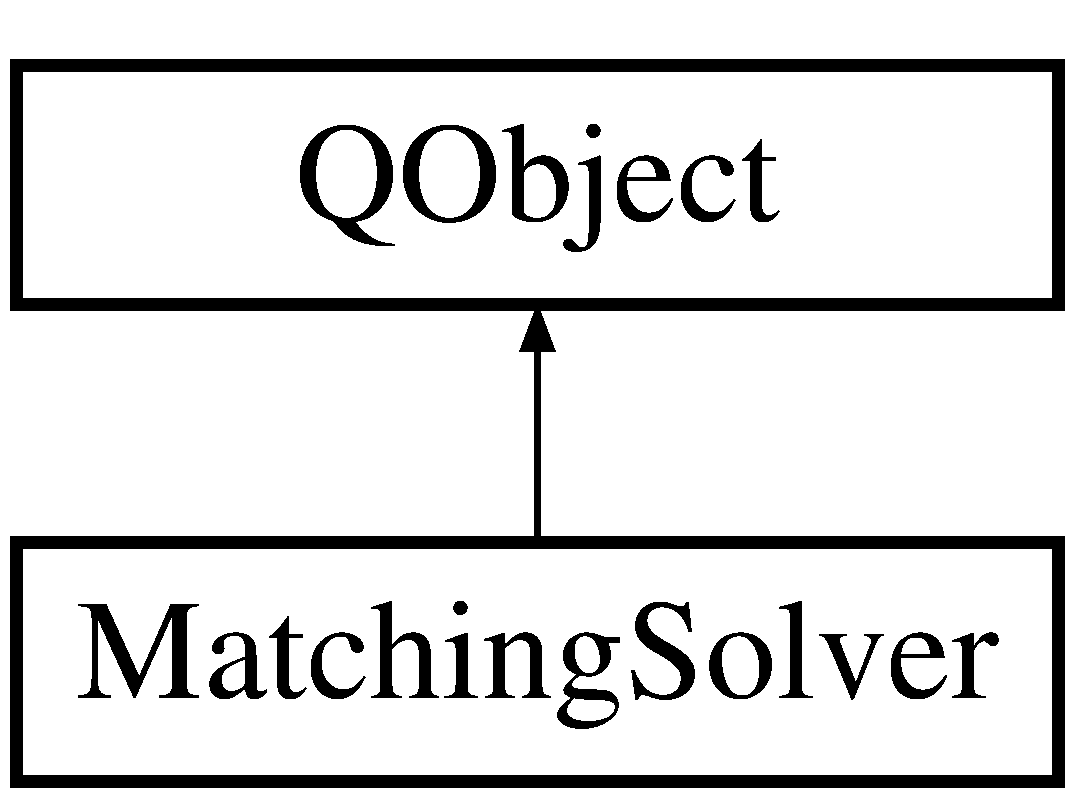
\includegraphics[height=2.000000cm]{classMatchingSolver}
\end{center}
\end{figure}
\subsection*{Public Slots}
\begin{DoxyCompactItemize}
\item 
void \hyperlink{classMatchingSolver_afbd9f5c5ad885d89a319f751df5beaad}{get\-Random\-Solution} ()
\item 
void \hyperlink{classMatchingSolver_ac69e6c3f40d3df7c55e5ff7d307acacc}{interrupt} ()
\end{DoxyCompactItemize}
\subsection*{Signals}
\begin{DoxyCompactItemize}
\item 
void \hyperlink{classMatchingSolver_a4636879fe14fc8d2b5e41dd6be4a9eed}{finished} (\hyperlink{classSeatToSpeakerMapper}{Seat\-To\-Speaker\-Mapper} $\ast$mapper)
\begin{DoxyCompactList}\small\item\em Emitted after a solution was found. \end{DoxyCompactList}\item 
\hypertarget{classMatchingSolver_a8d685c64a6f848b0a3d8f42f5fe9a216}{void \hyperlink{classMatchingSolver_a8d685c64a6f848b0a3d8f42f5fe9a216}{interrupted} ()}\label{classMatchingSolver_a8d685c64a6f848b0a3d8f42f5fe9a216}

\begin{DoxyCompactList}\small\item\em Emitted after a successfull interrupt. \end{DoxyCompactList}\item 
void \hyperlink{classMatchingSolver_aaf7b8cbfb8ee9a55ef5a10bc20ef5e7a}{no\-Solution\-Found} (Q\-String\-List errors)
\begin{DoxyCompactList}\small\item\em Emitted if no feasible solution exists. \end{DoxyCompactList}\item 
void \hyperlink{classMatchingSolver_af02dc51033a7a381855a1bd6fd77a39c}{done} ()
\end{DoxyCompactItemize}
\subsection*{Public Member Functions}
\begin{DoxyCompactItemize}
\item 
\hyperlink{classMatchingSolver_a0b9694c01fe96c7586f218dd11f7e9bc}{Matching\-Solver} (const Q\-List$<$ \hyperlink{classDebate}{Debate} $\ast$ $>$ $\ast$debates, const Q\-List$<$ \hyperlink{classSpeakerModel}{Speaker\-Model} $\ast$ $>$ $\ast$speakers, const Q\-List$<$ \hyperlink{classTeam}{Team} $\ast$ $>$ $\ast$teams, Q\-Object $\ast$parent)
\begin{DoxyCompactList}\small\item\em \hyperlink{classMatchingSolver}{Matching\-Solver} creates a new matching solver with given problem data. \end{DoxyCompactList}\item 
\hypertarget{classMatchingSolver_ad58841ead4b492150652e807e7ac4181}{bool \hyperlink{classMatchingSolver_ad58841ead4b492150652e807e7ac4181}{is\-Interrupted} ()}\label{classMatchingSolver_ad58841ead4b492150652e807e7ac4181}

\begin{DoxyCompactList}\small\item\em Returns {\ttfamily true} if the solver was interrupted. \end{DoxyCompactList}\end{DoxyCompactItemize}


\subsection{Detailed Description}
Solves the main D\-D\-T matching problem. 

D\-D\-T matches speakers to speaker roles in a debate. Only feasible matchings will be calculated, otherwise the solver signals that no solution exists. A matching is only feasible if
\begin{DoxyItemize}
\item No speaker is mapped to a role that is not allowed for him (e.\-g. by setting \hyperlink{classSpeakerModel_ae7ddef47cf54a9ace7c2399c7a18049d}{Speaker\-Model\-::opd\-Ffr} to false
\item Two beginner must not be placed in the same team
\item Teams must be placed in the same team The computational complexity of the problem hight due to the last two feasability criteria. This class uses google's constraint programming solver  or-\/tools to calculate optimal solutions.\par
The solver is not designed to calculate all solutions (the number of solutions grows exponentionally with the number of speakers) but guarantees highly randomised single solutions by shuffling the input data. New random solutions can be obtained without recreating the solver. \par
The class is designed to operate in its own thread, communication is done by Qt's signal/slot mechanism. 
\end{DoxyItemize}

\subsection{Constructor \& Destructor Documentation}
\hypertarget{classMatchingSolver_a0b9694c01fe96c7586f218dd11f7e9bc}{\index{Matching\-Solver@{Matching\-Solver}!Matching\-Solver@{Matching\-Solver}}
\index{Matching\-Solver@{Matching\-Solver}!MatchingSolver@{Matching\-Solver}}
\subsubsection[{Matching\-Solver}]{\setlength{\rightskip}{0pt plus 5cm}Matching\-Solver\-::\-Matching\-Solver (
\begin{DoxyParamCaption}
\item[{const Q\-List$<$ {\bf Debate} $\ast$ $>$ $\ast$}]{debates, }
\item[{const Q\-List$<$ {\bf Speaker\-Model} $\ast$ $>$ $\ast$}]{speakers, }
\item[{const Q\-List$<$ {\bf Team} $\ast$ $>$ $\ast$}]{teams, }
\item[{Q\-Object $\ast$}]{parent}
\end{DoxyParamCaption}
)}}\label{classMatchingSolver_a0b9694c01fe96c7586f218dd11f7e9bc}


\hyperlink{classMatchingSolver}{Matching\-Solver} creates a new matching solver with given problem data. 


\begin{DoxyParams}{Parameters}
{\em debates} & The debates considered for this matching. \\
\hline
{\em speakers} & The speakers considered for this matching. \\
\hline
{\em teams} & The teams considered for this matching. \\
\hline
{\em parent} & The solver's parent object \\
\hline
\end{DoxyParams}


\subsection{Member Function Documentation}
\hypertarget{classMatchingSolver_af02dc51033a7a381855a1bd6fd77a39c}{\index{Matching\-Solver@{Matching\-Solver}!done@{done}}
\index{done@{done}!MatchingSolver@{Matching\-Solver}}
\subsubsection[{done}]{\setlength{\rightskip}{0pt plus 5cm}void Matching\-Solver\-::done (
\begin{DoxyParamCaption}
{}
\end{DoxyParamCaption}
)\hspace{0.3cm}{\ttfamily [signal]}}}\label{classMatchingSolver_af02dc51033a7a381855a1bd6fd77a39c}
Called after either \hyperlink{classMatchingSolver_a4636879fe14fc8d2b5e41dd6be4a9eed}{finished}, \hyperlink{classMatchingSolver_a8d685c64a6f848b0a3d8f42f5fe9a216}{interrupted} or \hyperlink{classMatchingSolver_aaf7b8cbfb8ee9a55ef5a10bc20ef5e7a}{no\-Solution\-Found} have been called. The solver becomes inactive afterwards. \hypertarget{classMatchingSolver_a4636879fe14fc8d2b5e41dd6be4a9eed}{\index{Matching\-Solver@{Matching\-Solver}!finished@{finished}}
\index{finished@{finished}!MatchingSolver@{Matching\-Solver}}
\subsubsection[{finished}]{\setlength{\rightskip}{0pt plus 5cm}void Matching\-Solver\-::finished (
\begin{DoxyParamCaption}
\item[{{\bf Seat\-To\-Speaker\-Mapper} $\ast$}]{mapper}
\end{DoxyParamCaption}
)\hspace{0.3cm}{\ttfamily [signal]}}}\label{classMatchingSolver_a4636879fe14fc8d2b5e41dd6be4a9eed}


Emitted after a solution was found. 


\begin{DoxyParams}{Parameters}
{\em mapper} & a feasible, freshly calculated solution. \\
\hline
\end{DoxyParams}
\hypertarget{classMatchingSolver_afbd9f5c5ad885d89a319f751df5beaad}{\index{Matching\-Solver@{Matching\-Solver}!get\-Random\-Solution@{get\-Random\-Solution}}
\index{get\-Random\-Solution@{get\-Random\-Solution}!MatchingSolver@{Matching\-Solver}}
\subsubsection[{get\-Random\-Solution}]{\setlength{\rightskip}{0pt plus 5cm}void Matching\-Solver\-::get\-Random\-Solution (
\begin{DoxyParamCaption}
{}
\end{DoxyParamCaption}
)\hspace{0.3cm}{\ttfamily [slot]}}}\label{classMatchingSolver_afbd9f5c5ad885d89a319f751df5beaad}
Starts the calculation of a new random solution. Once the calculation is finished, \hyperlink{classMatchingSolver_aaf7b8cbfb8ee9a55ef5a10bc20ef5e7a}{no\-Solution\-Found} or \hyperlink{classMatchingSolver_a4636879fe14fc8d2b5e41dd6be4a9eed}{finished} is signaled. \hypertarget{classMatchingSolver_ac69e6c3f40d3df7c55e5ff7d307acacc}{\index{Matching\-Solver@{Matching\-Solver}!interrupt@{interrupt}}
\index{interrupt@{interrupt}!MatchingSolver@{Matching\-Solver}}
\subsubsection[{interrupt}]{\setlength{\rightskip}{0pt plus 5cm}void Matching\-Solver\-::interrupt (
\begin{DoxyParamCaption}
{}
\end{DoxyParamCaption}
)\hspace{0.3cm}{\ttfamily [slot]}}}\label{classMatchingSolver_ac69e6c3f40d3df7c55e5ff7d307acacc}
Asks the solver to interrupt the current solving process. The call has no effect if no calculation is running. After a succesfull interrupt, \hyperlink{classMatchingSolver_a8d685c64a6f848b0a3d8f42f5fe9a216}{interrupted} is signaled. \hypertarget{classMatchingSolver_aaf7b8cbfb8ee9a55ef5a10bc20ef5e7a}{\index{Matching\-Solver@{Matching\-Solver}!no\-Solution\-Found@{no\-Solution\-Found}}
\index{no\-Solution\-Found@{no\-Solution\-Found}!MatchingSolver@{Matching\-Solver}}
\subsubsection[{no\-Solution\-Found}]{\setlength{\rightskip}{0pt plus 5cm}void Matching\-Solver\-::no\-Solution\-Found (
\begin{DoxyParamCaption}
\item[{Q\-String\-List}]{errors}
\end{DoxyParamCaption}
)\hspace{0.3cm}{\ttfamily [signal]}}}\label{classMatchingSolver_aaf7b8cbfb8ee9a55ef5a10bc20ef5e7a}


Emitted if no feasible solution exists. 


\begin{DoxyParams}{Parameters}
{\em errors} & a (potentially empty) list of reasons why no solution could be found. \\
\hline
\end{DoxyParams}


The documentation for this class was generated from the following files\-:\begin{DoxyCompactItemize}
\item 
/home/stoef/qt/projects/ddt/ddt/src/matchingsolver.\-h\item 
/home/stoef/qt/projects/ddt/ddt/src/matchingsolver.\-cpp\end{DoxyCompactItemize}

\hypertarget{classMixedValueSpeakerModel}{\section{Mixed\-Value\-Speaker\-Model Class Reference}
\label{classMixedValueSpeakerModel}\index{Mixed\-Value\-Speaker\-Model@{Mixed\-Value\-Speaker\-Model}}
}


Allows editing multiple speakers at once.  




{\ttfamily \#include $<$mixedvaluespeakermodel.\-h$>$}

Inheritance diagram for Mixed\-Value\-Speaker\-Model\-:\begin{figure}[H]
\begin{center}
\leavevmode
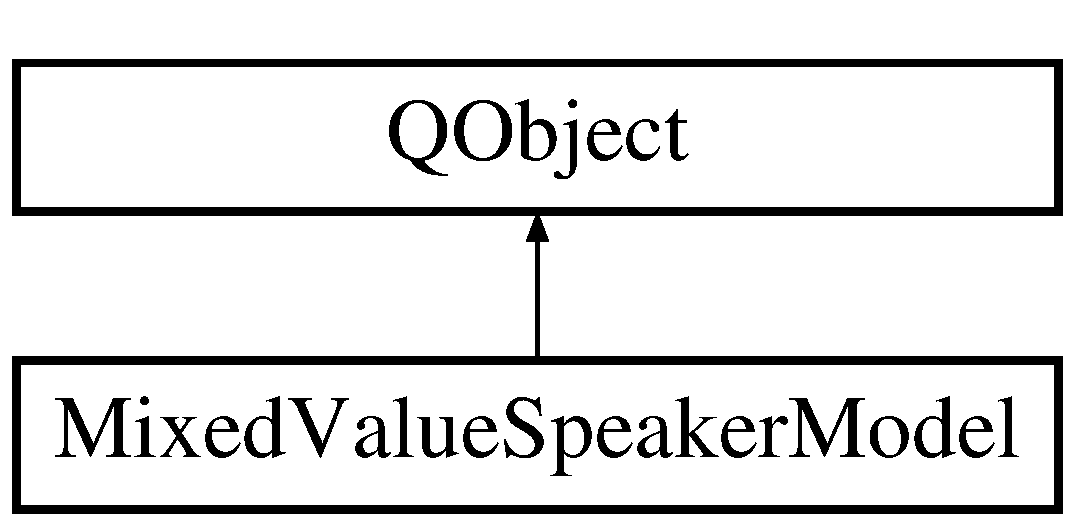
\includegraphics[height=2.000000cm]{classMixedValueSpeakerModel}
\end{center}
\end{figure}
\subsection*{Public Types}
\begin{DoxyCompactItemize}
\item 
enum \hyperlink{classMixedValueSpeakerModel_a37c5eeb40e2cbb783e862bd46248581e}{Property\-Id} \{ \\*
\hyperlink{classMixedValueSpeakerModel_a37c5eeb40e2cbb783e862bd46248581ea773e960b2075e59272ffc5686d355fbd}{O\-P\-D\-\_\-\-F\-F\-R\-\_\-\-I\-D}, 
\hyperlink{classMixedValueSpeakerModel_a37c5eeb40e2cbb783e862bd46248581ea64446396a42ef7101fd767269e83892d}{O\-P\-D\-\_\-\-G\-O\-V\-\_\-\-I\-D}, 
\hyperlink{classMixedValueSpeakerModel_a37c5eeb40e2cbb783e862bd46248581eacd70ceb54acb7b287509a33f46789afd}{O\-P\-D\-\_\-\-O\-P\-\_\-\-I\-D}, 
\hyperlink{classMixedValueSpeakerModel_a37c5eeb40e2cbb783e862bd46248581ea5b6f81bda4b8e3ca7a8768f717bb8b98}{B\-P\-S\-\_\-\-G\-O\-V\-\_\-\-I\-D}, 
\\*
\hyperlink{classMixedValueSpeakerModel_a37c5eeb40e2cbb783e862bd46248581ea6af44ca6adc89e03d4cabe42cfe243e4}{B\-P\-S\-\_\-\-O\-P\-\_\-\-I\-D}, 
\hyperlink{classMixedValueSpeakerModel_a37c5eeb40e2cbb783e862bd46248581ea7c1e5bc6d62d255e4f983444c2117e2f}{O\-P\-D\-\_\-\-J\-U\-D\-\_\-\-I\-D}, 
\hyperlink{classMixedValueSpeakerModel_a37c5eeb40e2cbb783e862bd46248581ea52f5599056ee645f34c3a304877c99c1}{B\-P\-S\-\_\-\-J\-U\-D\-\_\-\-I\-D}, 
\hyperlink{classMixedValueSpeakerModel_a37c5eeb40e2cbb783e862bd46248581ea694f3de82d85241a14a5b32226f73439}{I\-S\-\_\-\-B\-E\-G\-I\-N\-N\-E\-R\-\_\-\-I\-D}
 \}
\item 
enum \hyperlink{classMixedValueSpeakerModel_ab53ddbef6944a7444b39801fb4cf07f1}{Property\-State} \{ \hyperlink{classMixedValueSpeakerModel_ab53ddbef6944a7444b39801fb4cf07f1a2f795f14f329ea6f5b5cd5f3621c5ed4}{O\-F\-F}, 
\hyperlink{classMixedValueSpeakerModel_ab53ddbef6944a7444b39801fb4cf07f1a482016d67e200911b64b2a4dfd6aef12}{O\-N}, 
\hyperlink{classMixedValueSpeakerModel_ab53ddbef6944a7444b39801fb4cf07f1afa6f77f153e563f51999d02bc7777d30}{U\-N\-D\-E\-F\-I\-N\-E\-D}, 
\hyperlink{classMixedValueSpeakerModel_ab53ddbef6944a7444b39801fb4cf07f1a722e0e8c9fa60ac97ac70cbf9cdfb1a3}{M\-I\-X\-E\-D}
 \}
\end{DoxyCompactItemize}
\subsection*{Public Slots}
\begin{DoxyCompactItemize}
\item 
\hypertarget{classMixedValueSpeakerModel_a2923e98af84c0e75fb38e8863971490d}{void {\bfseries rows\-Inserted} (Q\-Model\-Index, int start, int end)}\label{classMixedValueSpeakerModel_a2923e98af84c0e75fb38e8863971490d}

\item 
\hypertarget{classMixedValueSpeakerModel_a64c72937cfb59485bd48e37aaccd3dee}{void {\bfseries rows\-Removed} (Q\-Model\-Index, int start, int end)}\label{classMixedValueSpeakerModel_a64c72937cfb59485bd48e37aaccd3dee}

\end{DoxyCompactItemize}
\subsection*{Signals}
\begin{DoxyCompactItemize}
\item 
\hypertarget{classMixedValueSpeakerModel_a1da3109c50fe8ec02982f876874cc839}{void {\bfseries is\-Beginner\-Changed} ()}\label{classMixedValueSpeakerModel_a1da3109c50fe8ec02982f876874cc839}

\item 
\hypertarget{classMixedValueSpeakerModel_a73cd75a2b22d43f51d020bb67621acc6}{void {\bfseries opd\-Ffr\-Changed} ()}\label{classMixedValueSpeakerModel_a73cd75a2b22d43f51d020bb67621acc6}

\item 
\hypertarget{classMixedValueSpeakerModel_adcd7c48db0f30b9052e1e66950efd950}{void {\bfseries opd\-Gov\-Changed} ()}\label{classMixedValueSpeakerModel_adcd7c48db0f30b9052e1e66950efd950}

\item 
\hypertarget{classMixedValueSpeakerModel_a02d3b7f9362a9aa88c981799142bb788}{void {\bfseries opd\-Op\-Changed} ()}\label{classMixedValueSpeakerModel_a02d3b7f9362a9aa88c981799142bb788}

\item 
\hypertarget{classMixedValueSpeakerModel_a4af16e965bc4298857666a156bd16b49}{void {\bfseries bps\-Gov\-Changed} ()}\label{classMixedValueSpeakerModel_a4af16e965bc4298857666a156bd16b49}

\item 
\hypertarget{classMixedValueSpeakerModel_aa5f650827dfb02fbeb40dd4651c782fe}{void {\bfseries bps\-Op\-Changed} ()}\label{classMixedValueSpeakerModel_aa5f650827dfb02fbeb40dd4651c782fe}

\item 
\hypertarget{classMixedValueSpeakerModel_a2fe989cd11ad486b16136c00dbe7ca35}{void {\bfseries opd\-Jud\-Changed} ()}\label{classMixedValueSpeakerModel_a2fe989cd11ad486b16136c00dbe7ca35}

\item 
\hypertarget{classMixedValueSpeakerModel_ad70d654da71d9992ceca901db8efd1ed}{void {\bfseries bps\-Jud\-Changed} ()}\label{classMixedValueSpeakerModel_ad70d654da71d9992ceca901db8efd1ed}

\end{DoxyCompactItemize}
\subsection*{Public Member Functions}
\begin{DoxyCompactItemize}
\item 
\hypertarget{classMixedValueSpeakerModel_abc6e28bb88a03b21860d0762a0955394}{{\bfseries Mixed\-Value\-Speaker\-Model} (Q\-Object $\ast$parent=0)}\label{classMixedValueSpeakerModel_abc6e28bb88a03b21860d0762a0955394}

\item 
\hypertarget{classMixedValueSpeakerModel_a15eebfa3e351f372138ca73f4984e636}{\hyperlink{classMixedValueSpeakerModel_ab53ddbef6944a7444b39801fb4cf07f1}{Property\-State} {\bfseries is\-Beginner} ()}\label{classMixedValueSpeakerModel_a15eebfa3e351f372138ca73f4984e636}

\item 
\hypertarget{classMixedValueSpeakerModel_add4596cd0fe2412a7404251b86d74269}{\hyperlink{classMixedValueSpeakerModel_ab53ddbef6944a7444b39801fb4cf07f1}{Property\-State} {\bfseries opd\-Ffr} ()}\label{classMixedValueSpeakerModel_add4596cd0fe2412a7404251b86d74269}

\item 
\hypertarget{classMixedValueSpeakerModel_a1da4d799d894032c1523f4b8f450e31d}{\hyperlink{classMixedValueSpeakerModel_ab53ddbef6944a7444b39801fb4cf07f1}{Property\-State} {\bfseries opd\-Gov} ()}\label{classMixedValueSpeakerModel_a1da4d799d894032c1523f4b8f450e31d}

\item 
\hypertarget{classMixedValueSpeakerModel_a55952e37bd67e014cca8a06a17f337c6}{\hyperlink{classMixedValueSpeakerModel_ab53ddbef6944a7444b39801fb4cf07f1}{Property\-State} {\bfseries opd\-Op} ()}\label{classMixedValueSpeakerModel_a55952e37bd67e014cca8a06a17f337c6}

\item 
\hypertarget{classMixedValueSpeakerModel_a2336f30f032bcecde416263996a8cda4}{\hyperlink{classMixedValueSpeakerModel_ab53ddbef6944a7444b39801fb4cf07f1}{Property\-State} {\bfseries bps\-Gov} ()}\label{classMixedValueSpeakerModel_a2336f30f032bcecde416263996a8cda4}

\item 
\hypertarget{classMixedValueSpeakerModel_a5e9b70338e3c9d657246760b42dc2b7d}{\hyperlink{classMixedValueSpeakerModel_ab53ddbef6944a7444b39801fb4cf07f1}{Property\-State} {\bfseries bps\-Op} ()}\label{classMixedValueSpeakerModel_a5e9b70338e3c9d657246760b42dc2b7d}

\item 
\hypertarget{classMixedValueSpeakerModel_a61d941fb2ae0971bd12103fae043c2ed}{\hyperlink{classMixedValueSpeakerModel_ab53ddbef6944a7444b39801fb4cf07f1}{Property\-State} {\bfseries opd\-Jud} ()}\label{classMixedValueSpeakerModel_a61d941fb2ae0971bd12103fae043c2ed}

\item 
\hypertarget{classMixedValueSpeakerModel_a5e4498aff43997d219ede6199cbedfcf}{\hyperlink{classMixedValueSpeakerModel_ab53ddbef6944a7444b39801fb4cf07f1}{Property\-State} {\bfseries bps\-Jud} ()}\label{classMixedValueSpeakerModel_a5e4498aff43997d219ede6199cbedfcf}

\item 
\hypertarget{classMixedValueSpeakerModel_a8a95e8da0d76aba08463d127c0a758fb}{void {\bfseries set\-Selection\-Model} (\hyperlink{classQListQmlWrapper}{Q\-List\-Qml\-Wrapper} $\ast$\hyperlink{classMixedValueSpeakerModel_a58e2d9f253efcec1338b063636f671c7}{selection\-Model})}\label{classMixedValueSpeakerModel_a8a95e8da0d76aba08463d127c0a758fb}

\item 
Q\-\_\-\-I\-N\-V\-O\-K\-A\-B\-L\-E void \hyperlink{classMixedValueSpeakerModel_a75dca37807957d62e0327ff183abcd31}{set\-Multi\-Property} (\hyperlink{classMixedValueSpeakerModel_a37c5eeb40e2cbb783e862bd46248581e}{Property\-Id} id, bool new\-Value)
\begin{DoxyCompactList}\small\item\em Sets a bool property of all currently selected speakers to a new value. \end{DoxyCompactList}\end{DoxyCompactItemize}
\subsection*{Properties}
\begin{DoxyCompactItemize}
\item 
\hyperlink{classQListQmlWrapper}{Q\-List\-Qml\-Wrapper} \hyperlink{classMixedValueSpeakerModel_a58e2d9f253efcec1338b063636f671c7}{selection\-Model}
\item 
\hyperlink{classMixedValueSpeakerModel_ab53ddbef6944a7444b39801fb4cf07f1}{Property\-State} \hyperlink{classMixedValueSpeakerModel_aa975aa5cc1bc9ce5cf271bdde100956f}{is\-Beginner}
\item 
\hyperlink{classMixedValueSpeakerModel_ab53ddbef6944a7444b39801fb4cf07f1}{Property\-State} \hyperlink{classMixedValueSpeakerModel_ae15c206a56abfba981224678d4b5b275}{opd\-Ffr}
\item 
\hyperlink{classMixedValueSpeakerModel_ab53ddbef6944a7444b39801fb4cf07f1}{Property\-State} \hyperlink{classMixedValueSpeakerModel_a78a4add3e011e2a5b4632f751f9d9b86}{opd\-Gov}
\item 
\hyperlink{classMixedValueSpeakerModel_ab53ddbef6944a7444b39801fb4cf07f1}{Property\-State} \hyperlink{classMixedValueSpeakerModel_a4da92388fbadb9aa5091d80f99078404}{opd\-Op}
\item 
\hyperlink{classMixedValueSpeakerModel_ab53ddbef6944a7444b39801fb4cf07f1}{Property\-State} \hyperlink{classMixedValueSpeakerModel_af0623f60ccedd60ef1ab06718a4edbdb}{bps\-Gov}
\item 
\hyperlink{classMixedValueSpeakerModel_ab53ddbef6944a7444b39801fb4cf07f1}{Property\-State} \hyperlink{classMixedValueSpeakerModel_a0dc7854f44ae909f8908bacb8f93da4c}{bps\-Op}
\item 
\hyperlink{classMixedValueSpeakerModel_ab53ddbef6944a7444b39801fb4cf07f1}{Property\-State} \hyperlink{classMixedValueSpeakerModel_ad7a22ac891701f43d71a0ee50647f41f}{opd\-Jud}
\item 
\hyperlink{classMixedValueSpeakerModel_ab53ddbef6944a7444b39801fb4cf07f1}{Property\-State} \hyperlink{classMixedValueSpeakerModel_aa39c027299f39cdaf188052a41d4dc69}{bps\-Jud}
\end{DoxyCompactItemize}


\subsection{Detailed Description}
Allows editing multiple speakers at once. 

{\ttfamily \hyperlink{classMixedValueSpeakerModel}{Mixed\-Value\-Speaker\-Model}} has an interface similar to \hyperlink{classSpeakerModel}{Speaker\-Model}, it contains all its boolean typed properties. It accesses a list of different {\ttfamily \hyperlink{classSpeakerModel}{Speaker\-Model}} and combines their properties. If the list contains different values for some property, Property\-State\-::\-M\-I\-X\-E\-D will be returned as the property's value. Moreover, setting some property for all speakers at once is possible. 

\subsection{Member Enumeration Documentation}
\hypertarget{classMixedValueSpeakerModel_a37c5eeb40e2cbb783e862bd46248581e}{\index{Mixed\-Value\-Speaker\-Model@{Mixed\-Value\-Speaker\-Model}!Property\-Id@{Property\-Id}}
\index{Property\-Id@{Property\-Id}!MixedValueSpeakerModel@{Mixed\-Value\-Speaker\-Model}}
\subsubsection[{Property\-Id}]{\setlength{\rightskip}{0pt plus 5cm}enum {\bf Mixed\-Value\-Speaker\-Model\-::\-Property\-Id}}}\label{classMixedValueSpeakerModel_a37c5eeb40e2cbb783e862bd46248581e}
Instead of offering setters for all propertie's, only one setter is given.  is used to specify the property that should be set. \begin{DoxySeeAlso}{See Also}
\hyperlink{classMixedValueSpeakerModel_a75dca37807957d62e0327ff183abcd31}{set\-Multi\-Property} 
\end{DoxySeeAlso}
\begin{Desc}
\item[Enumerator]\par
\begin{description}
\index{O\-P\-D\-\_\-\-F\-F\-R\-\_\-\-I\-D@{O\-P\-D\-\_\-\-F\-F\-R\-\_\-\-I\-D}!Mixed\-Value\-Speaker\-Model@{Mixed\-Value\-Speaker\-Model}}\index{Mixed\-Value\-Speaker\-Model@{Mixed\-Value\-Speaker\-Model}!O\-P\-D\-\_\-\-F\-F\-R\-\_\-\-I\-D@{O\-P\-D\-\_\-\-F\-F\-R\-\_\-\-I\-D}}\item[{\em 
\hypertarget{classMixedValueSpeakerModel_a37c5eeb40e2cbb783e862bd46248581ea773e960b2075e59272ffc5686d355fbd}{O\-P\-D\-\_\-\-F\-F\-R\-\_\-\-I\-D}\label{classMixedValueSpeakerModel_a37c5eeb40e2cbb783e862bd46248581ea773e960b2075e59272ffc5686d355fbd}
}]Used to edit \hyperlink{classSpeakerModel_ae7ddef47cf54a9ace7c2399c7a18049d}{Speaker\-Model\-::opd\-Ffr} \index{O\-P\-D\-\_\-\-G\-O\-V\-\_\-\-I\-D@{O\-P\-D\-\_\-\-G\-O\-V\-\_\-\-I\-D}!Mixed\-Value\-Speaker\-Model@{Mixed\-Value\-Speaker\-Model}}\index{Mixed\-Value\-Speaker\-Model@{Mixed\-Value\-Speaker\-Model}!O\-P\-D\-\_\-\-G\-O\-V\-\_\-\-I\-D@{O\-P\-D\-\_\-\-G\-O\-V\-\_\-\-I\-D}}\item[{\em 
\hypertarget{classMixedValueSpeakerModel_a37c5eeb40e2cbb783e862bd46248581ea64446396a42ef7101fd767269e83892d}{O\-P\-D\-\_\-\-G\-O\-V\-\_\-\-I\-D}\label{classMixedValueSpeakerModel_a37c5eeb40e2cbb783e862bd46248581ea64446396a42ef7101fd767269e83892d}
}]Used to edit \hyperlink{classSpeakerModel_a7a7dafddf0d9f0bb60e5e138277b50fd}{Speaker\-Model\-::opd\-Gov} \index{O\-P\-D\-\_\-\-O\-P\-\_\-\-I\-D@{O\-P\-D\-\_\-\-O\-P\-\_\-\-I\-D}!Mixed\-Value\-Speaker\-Model@{Mixed\-Value\-Speaker\-Model}}\index{Mixed\-Value\-Speaker\-Model@{Mixed\-Value\-Speaker\-Model}!O\-P\-D\-\_\-\-O\-P\-\_\-\-I\-D@{O\-P\-D\-\_\-\-O\-P\-\_\-\-I\-D}}\item[{\em 
\hypertarget{classMixedValueSpeakerModel_a37c5eeb40e2cbb783e862bd46248581eacd70ceb54acb7b287509a33f46789afd}{O\-P\-D\-\_\-\-O\-P\-\_\-\-I\-D}\label{classMixedValueSpeakerModel_a37c5eeb40e2cbb783e862bd46248581eacd70ceb54acb7b287509a33f46789afd}
}]Used to edit \hyperlink{classSpeakerModel_a60ebe1609153ba734e8d5449643cd85e}{Speaker\-Model\-::opd\-Op} \index{B\-P\-S\-\_\-\-G\-O\-V\-\_\-\-I\-D@{B\-P\-S\-\_\-\-G\-O\-V\-\_\-\-I\-D}!Mixed\-Value\-Speaker\-Model@{Mixed\-Value\-Speaker\-Model}}\index{Mixed\-Value\-Speaker\-Model@{Mixed\-Value\-Speaker\-Model}!B\-P\-S\-\_\-\-G\-O\-V\-\_\-\-I\-D@{B\-P\-S\-\_\-\-G\-O\-V\-\_\-\-I\-D}}\item[{\em 
\hypertarget{classMixedValueSpeakerModel_a37c5eeb40e2cbb783e862bd46248581ea5b6f81bda4b8e3ca7a8768f717bb8b98}{B\-P\-S\-\_\-\-G\-O\-V\-\_\-\-I\-D}\label{classMixedValueSpeakerModel_a37c5eeb40e2cbb783e862bd46248581ea5b6f81bda4b8e3ca7a8768f717bb8b98}
}]Used to edit \hyperlink{classSpeakerModel_aaf2dd2737f827659f7ca2a8a6b8a87f3}{Speaker\-Model\-::bps\-Gov} \index{B\-P\-S\-\_\-\-O\-P\-\_\-\-I\-D@{B\-P\-S\-\_\-\-O\-P\-\_\-\-I\-D}!Mixed\-Value\-Speaker\-Model@{Mixed\-Value\-Speaker\-Model}}\index{Mixed\-Value\-Speaker\-Model@{Mixed\-Value\-Speaker\-Model}!B\-P\-S\-\_\-\-O\-P\-\_\-\-I\-D@{B\-P\-S\-\_\-\-O\-P\-\_\-\-I\-D}}\item[{\em 
\hypertarget{classMixedValueSpeakerModel_a37c5eeb40e2cbb783e862bd46248581ea6af44ca6adc89e03d4cabe42cfe243e4}{B\-P\-S\-\_\-\-O\-P\-\_\-\-I\-D}\label{classMixedValueSpeakerModel_a37c5eeb40e2cbb783e862bd46248581ea6af44ca6adc89e03d4cabe42cfe243e4}
}]Used to edit Speaker\-Model\-::bps\-Opd \index{O\-P\-D\-\_\-\-J\-U\-D\-\_\-\-I\-D@{O\-P\-D\-\_\-\-J\-U\-D\-\_\-\-I\-D}!Mixed\-Value\-Speaker\-Model@{Mixed\-Value\-Speaker\-Model}}\index{Mixed\-Value\-Speaker\-Model@{Mixed\-Value\-Speaker\-Model}!O\-P\-D\-\_\-\-J\-U\-D\-\_\-\-I\-D@{O\-P\-D\-\_\-\-J\-U\-D\-\_\-\-I\-D}}\item[{\em 
\hypertarget{classMixedValueSpeakerModel_a37c5eeb40e2cbb783e862bd46248581ea7c1e5bc6d62d255e4f983444c2117e2f}{O\-P\-D\-\_\-\-J\-U\-D\-\_\-\-I\-D}\label{classMixedValueSpeakerModel_a37c5eeb40e2cbb783e862bd46248581ea7c1e5bc6d62d255e4f983444c2117e2f}
}]Used to edit \hyperlink{classSpeakerModel_a427f9e7d98bcbaea06f395eb82271a56}{Speaker\-Model\-::opd\-Jud} \index{B\-P\-S\-\_\-\-J\-U\-D\-\_\-\-I\-D@{B\-P\-S\-\_\-\-J\-U\-D\-\_\-\-I\-D}!Mixed\-Value\-Speaker\-Model@{Mixed\-Value\-Speaker\-Model}}\index{Mixed\-Value\-Speaker\-Model@{Mixed\-Value\-Speaker\-Model}!B\-P\-S\-\_\-\-J\-U\-D\-\_\-\-I\-D@{B\-P\-S\-\_\-\-J\-U\-D\-\_\-\-I\-D}}\item[{\em 
\hypertarget{classMixedValueSpeakerModel_a37c5eeb40e2cbb783e862bd46248581ea52f5599056ee645f34c3a304877c99c1}{B\-P\-S\-\_\-\-J\-U\-D\-\_\-\-I\-D}\label{classMixedValueSpeakerModel_a37c5eeb40e2cbb783e862bd46248581ea52f5599056ee645f34c3a304877c99c1}
}]Used to edit \hyperlink{classSpeakerModel_a60f2670dcde9e6dbe24661599e6b674c}{Speaker\-Model\-::bps\-Jud} \index{I\-S\-\_\-\-B\-E\-G\-I\-N\-N\-E\-R\-\_\-\-I\-D@{I\-S\-\_\-\-B\-E\-G\-I\-N\-N\-E\-R\-\_\-\-I\-D}!Mixed\-Value\-Speaker\-Model@{Mixed\-Value\-Speaker\-Model}}\index{Mixed\-Value\-Speaker\-Model@{Mixed\-Value\-Speaker\-Model}!I\-S\-\_\-\-B\-E\-G\-I\-N\-N\-E\-R\-\_\-\-I\-D@{I\-S\-\_\-\-B\-E\-G\-I\-N\-N\-E\-R\-\_\-\-I\-D}}\item[{\em 
\hypertarget{classMixedValueSpeakerModel_a37c5eeb40e2cbb783e862bd46248581ea694f3de82d85241a14a5b32226f73439}{I\-S\-\_\-\-B\-E\-G\-I\-N\-N\-E\-R\-\_\-\-I\-D}\label{classMixedValueSpeakerModel_a37c5eeb40e2cbb783e862bd46248581ea694f3de82d85241a14a5b32226f73439}
}]Used to edit \hyperlink{classSpeakerModel_a47d41be22317dd22fd7aec6240c731cf}{Speaker\-Model\-::is\-Beginner} \end{description}
\end{Desc}
\hypertarget{classMixedValueSpeakerModel_ab53ddbef6944a7444b39801fb4cf07f1}{\index{Mixed\-Value\-Speaker\-Model@{Mixed\-Value\-Speaker\-Model}!Property\-State@{Property\-State}}
\index{Property\-State@{Property\-State}!MixedValueSpeakerModel@{Mixed\-Value\-Speaker\-Model}}
\subsubsection[{Property\-State}]{\setlength{\rightskip}{0pt plus 5cm}enum {\bf Mixed\-Value\-Speaker\-Model\-::\-Property\-State}}}\label{classMixedValueSpeakerModel_ab53ddbef6944a7444b39801fb4cf07f1}
Identifies the mixed state of a property of all speakers contained in the selection model. \begin{Desc}
\item[Enumerator]\par
\begin{description}
\index{O\-F\-F@{O\-F\-F}!Mixed\-Value\-Speaker\-Model@{Mixed\-Value\-Speaker\-Model}}\index{Mixed\-Value\-Speaker\-Model@{Mixed\-Value\-Speaker\-Model}!O\-F\-F@{O\-F\-F}}\item[{\em 
\hypertarget{classMixedValueSpeakerModel_ab53ddbef6944a7444b39801fb4cf07f1a2f795f14f329ea6f5b5cd5f3621c5ed4}{O\-F\-F}\label{classMixedValueSpeakerModel_ab53ddbef6944a7444b39801fb4cf07f1a2f795f14f329ea6f5b5cd5f3621c5ed4}
}]All properties are set to false \index{O\-N@{O\-N}!Mixed\-Value\-Speaker\-Model@{Mixed\-Value\-Speaker\-Model}}\index{Mixed\-Value\-Speaker\-Model@{Mixed\-Value\-Speaker\-Model}!O\-N@{O\-N}}\item[{\em 
\hypertarget{classMixedValueSpeakerModel_ab53ddbef6944a7444b39801fb4cf07f1a482016d67e200911b64b2a4dfd6aef12}{O\-N}\label{classMixedValueSpeakerModel_ab53ddbef6944a7444b39801fb4cf07f1a482016d67e200911b64b2a4dfd6aef12}
}]All properties are set to true \index{U\-N\-D\-E\-F\-I\-N\-E\-D@{U\-N\-D\-E\-F\-I\-N\-E\-D}!Mixed\-Value\-Speaker\-Model@{Mixed\-Value\-Speaker\-Model}}\index{Mixed\-Value\-Speaker\-Model@{Mixed\-Value\-Speaker\-Model}!U\-N\-D\-E\-F\-I\-N\-E\-D@{U\-N\-D\-E\-F\-I\-N\-E\-D}}\item[{\em 
\hypertarget{classMixedValueSpeakerModel_ab53ddbef6944a7444b39801fb4cf07f1afa6f77f153e563f51999d02bc7777d30}{U\-N\-D\-E\-F\-I\-N\-E\-D}\label{classMixedValueSpeakerModel_ab53ddbef6944a7444b39801fb4cf07f1afa6f77f153e563f51999d02bc7777d30}
}]The selection model is empty \index{M\-I\-X\-E\-D@{M\-I\-X\-E\-D}!Mixed\-Value\-Speaker\-Model@{Mixed\-Value\-Speaker\-Model}}\index{Mixed\-Value\-Speaker\-Model@{Mixed\-Value\-Speaker\-Model}!M\-I\-X\-E\-D@{M\-I\-X\-E\-D}}\item[{\em 
\hypertarget{classMixedValueSpeakerModel_ab53ddbef6944a7444b39801fb4cf07f1a722e0e8c9fa60ac97ac70cbf9cdfb1a3}{M\-I\-X\-E\-D}\label{classMixedValueSpeakerModel_ab53ddbef6944a7444b39801fb4cf07f1a722e0e8c9fa60ac97ac70cbf9cdfb1a3}
}]The properties have multiple values \end{description}
\end{Desc}


\subsection{Member Function Documentation}
\hypertarget{classMixedValueSpeakerModel_a75dca37807957d62e0327ff183abcd31}{\index{Mixed\-Value\-Speaker\-Model@{Mixed\-Value\-Speaker\-Model}!set\-Multi\-Property@{set\-Multi\-Property}}
\index{set\-Multi\-Property@{set\-Multi\-Property}!MixedValueSpeakerModel@{Mixed\-Value\-Speaker\-Model}}
\subsubsection[{set\-Multi\-Property}]{\setlength{\rightskip}{0pt plus 5cm}void Mixed\-Value\-Speaker\-Model\-::set\-Multi\-Property (
\begin{DoxyParamCaption}
\item[{{\bf Property\-Id}}]{id, }
\item[{bool}]{new\-Value}
\end{DoxyParamCaption}
)}}\label{classMixedValueSpeakerModel_a75dca37807957d62e0327ff183abcd31}


Sets a bool property of all currently selected speakers to a new value. 


\begin{DoxyParams}{Parameters}
{\em id} & identifies the property that should be set \\
\hline
{\em new\-State} & the properties new value \\
\hline
\end{DoxyParams}


\subsection{Property Documentation}
\hypertarget{classMixedValueSpeakerModel_af0623f60ccedd60ef1ab06718a4edbdb}{\index{Mixed\-Value\-Speaker\-Model@{Mixed\-Value\-Speaker\-Model}!bps\-Gov@{bps\-Gov}}
\index{bps\-Gov@{bps\-Gov}!MixedValueSpeakerModel@{Mixed\-Value\-Speaker\-Model}}
\subsubsection[{bps\-Gov}]{\setlength{\rightskip}{0pt plus 5cm}{\bf Property\-State} Mixed\-Value\-Speaker\-Model\-::bps\-Gov\hspace{0.3cm}{\ttfamily [read]}}}\label{classMixedValueSpeakerModel_af0623f60ccedd60ef1ab06718a4edbdb}
\begin{DoxySeeAlso}{See Also}
\hyperlink{classSpeakerModel_aaf2dd2737f827659f7ca2a8a6b8a87f3}{Speaker\-Model\-::bps\-Gov} 
\end{DoxySeeAlso}
\hypertarget{classMixedValueSpeakerModel_aa39c027299f39cdaf188052a41d4dc69}{\index{Mixed\-Value\-Speaker\-Model@{Mixed\-Value\-Speaker\-Model}!bps\-Jud@{bps\-Jud}}
\index{bps\-Jud@{bps\-Jud}!MixedValueSpeakerModel@{Mixed\-Value\-Speaker\-Model}}
\subsubsection[{bps\-Jud}]{\setlength{\rightskip}{0pt plus 5cm}{\bf Property\-State} Mixed\-Value\-Speaker\-Model\-::bps\-Jud\hspace{0.3cm}{\ttfamily [read]}}}\label{classMixedValueSpeakerModel_aa39c027299f39cdaf188052a41d4dc69}
\begin{DoxySeeAlso}{See Also}
\hyperlink{classSpeakerModel_a60f2670dcde9e6dbe24661599e6b674c}{Speaker\-Model\-::bps\-Jud} 
\end{DoxySeeAlso}
\hypertarget{classMixedValueSpeakerModel_a0dc7854f44ae909f8908bacb8f93da4c}{\index{Mixed\-Value\-Speaker\-Model@{Mixed\-Value\-Speaker\-Model}!bps\-Op@{bps\-Op}}
\index{bps\-Op@{bps\-Op}!MixedValueSpeakerModel@{Mixed\-Value\-Speaker\-Model}}
\subsubsection[{bps\-Op}]{\setlength{\rightskip}{0pt plus 5cm}{\bf Property\-State} Mixed\-Value\-Speaker\-Model\-::bps\-Op\hspace{0.3cm}{\ttfamily [read]}}}\label{classMixedValueSpeakerModel_a0dc7854f44ae909f8908bacb8f93da4c}
\begin{DoxySeeAlso}{See Also}
\hyperlink{classSpeakerModel_a2f2cac7000658283ccf8d06683b64376}{Speaker\-Model\-::bps\-Op} 
\end{DoxySeeAlso}
\hypertarget{classMixedValueSpeakerModel_aa975aa5cc1bc9ce5cf271bdde100956f}{\index{Mixed\-Value\-Speaker\-Model@{Mixed\-Value\-Speaker\-Model}!is\-Beginner@{is\-Beginner}}
\index{is\-Beginner@{is\-Beginner}!MixedValueSpeakerModel@{Mixed\-Value\-Speaker\-Model}}
\subsubsection[{is\-Beginner}]{\setlength{\rightskip}{0pt plus 5cm}{\bf Property\-State} Mixed\-Value\-Speaker\-Model\-::is\-Beginner\hspace{0.3cm}{\ttfamily [read]}, {\ttfamily [write]}}}\label{classMixedValueSpeakerModel_aa975aa5cc1bc9ce5cf271bdde100956f}
\begin{DoxySeeAlso}{See Also}
\hyperlink{classSpeakerModel_a47d41be22317dd22fd7aec6240c731cf}{Speaker\-Model\-::is\-Beginner} 
\end{DoxySeeAlso}
\hypertarget{classMixedValueSpeakerModel_ae15c206a56abfba981224678d4b5b275}{\index{Mixed\-Value\-Speaker\-Model@{Mixed\-Value\-Speaker\-Model}!opd\-Ffr@{opd\-Ffr}}
\index{opd\-Ffr@{opd\-Ffr}!MixedValueSpeakerModel@{Mixed\-Value\-Speaker\-Model}}
\subsubsection[{opd\-Ffr}]{\setlength{\rightskip}{0pt plus 5cm}{\bf Property\-State} Mixed\-Value\-Speaker\-Model\-::opd\-Ffr\hspace{0.3cm}{\ttfamily [read]}}}\label{classMixedValueSpeakerModel_ae15c206a56abfba981224678d4b5b275}
\begin{DoxySeeAlso}{See Also}
\hyperlink{classSpeakerModel_ae7ddef47cf54a9ace7c2399c7a18049d}{Speaker\-Model\-::opd\-Ffr} 
\end{DoxySeeAlso}
\hypertarget{classMixedValueSpeakerModel_a78a4add3e011e2a5b4632f751f9d9b86}{\index{Mixed\-Value\-Speaker\-Model@{Mixed\-Value\-Speaker\-Model}!opd\-Gov@{opd\-Gov}}
\index{opd\-Gov@{opd\-Gov}!MixedValueSpeakerModel@{Mixed\-Value\-Speaker\-Model}}
\subsubsection[{opd\-Gov}]{\setlength{\rightskip}{0pt plus 5cm}{\bf Property\-State} Mixed\-Value\-Speaker\-Model\-::opd\-Gov\hspace{0.3cm}{\ttfamily [read]}}}\label{classMixedValueSpeakerModel_a78a4add3e011e2a5b4632f751f9d9b86}
\begin{DoxySeeAlso}{See Also}
\hyperlink{classSpeakerModel_a7a7dafddf0d9f0bb60e5e138277b50fd}{Speaker\-Model\-::opd\-Gov} 
\end{DoxySeeAlso}
\hypertarget{classMixedValueSpeakerModel_ad7a22ac891701f43d71a0ee50647f41f}{\index{Mixed\-Value\-Speaker\-Model@{Mixed\-Value\-Speaker\-Model}!opd\-Jud@{opd\-Jud}}
\index{opd\-Jud@{opd\-Jud}!MixedValueSpeakerModel@{Mixed\-Value\-Speaker\-Model}}
\subsubsection[{opd\-Jud}]{\setlength{\rightskip}{0pt plus 5cm}{\bf Property\-State} Mixed\-Value\-Speaker\-Model\-::opd\-Jud\hspace{0.3cm}{\ttfamily [read]}}}\label{classMixedValueSpeakerModel_ad7a22ac891701f43d71a0ee50647f41f}
\begin{DoxySeeAlso}{See Also}
\hyperlink{classSpeakerModel_a427f9e7d98bcbaea06f395eb82271a56}{Speaker\-Model\-::opd\-Jud} 
\end{DoxySeeAlso}
\hypertarget{classMixedValueSpeakerModel_a4da92388fbadb9aa5091d80f99078404}{\index{Mixed\-Value\-Speaker\-Model@{Mixed\-Value\-Speaker\-Model}!opd\-Op@{opd\-Op}}
\index{opd\-Op@{opd\-Op}!MixedValueSpeakerModel@{Mixed\-Value\-Speaker\-Model}}
\subsubsection[{opd\-Op}]{\setlength{\rightskip}{0pt plus 5cm}{\bf Property\-State} Mixed\-Value\-Speaker\-Model\-::opd\-Op\hspace{0.3cm}{\ttfamily [read]}}}\label{classMixedValueSpeakerModel_a4da92388fbadb9aa5091d80f99078404}
\begin{DoxySeeAlso}{See Also}
\hyperlink{classSpeakerModel_a60ebe1609153ba734e8d5449643cd85e}{Speaker\-Model\-::opd\-Op} 
\end{DoxySeeAlso}
\hypertarget{classMixedValueSpeakerModel_a58e2d9f253efcec1338b063636f671c7}{\index{Mixed\-Value\-Speaker\-Model@{Mixed\-Value\-Speaker\-Model}!selection\-Model@{selection\-Model}}
\index{selection\-Model@{selection\-Model}!MixedValueSpeakerModel@{Mixed\-Value\-Speaker\-Model}}
\subsubsection[{selection\-Model}]{\setlength{\rightskip}{0pt plus 5cm}{\bf Q\-List\-Qml\-Wrapper} Mixed\-Value\-Speaker\-Model\-::selection\-Model\hspace{0.3cm}{\ttfamily [write]}}}\label{classMixedValueSpeakerModel_a58e2d9f253efcec1338b063636f671c7}
The selection model. Updates to the selection will automatically be detected. It must contain elements of type \hyperlink{classSpeakerModel}{Speaker\-Model}, no element should be contained twice. 

The documentation for this class was generated from the following files\-:\begin{DoxyCompactItemize}
\item 
/home/stoef/qt/projects/ddt/ddt/src/mixedvaluespeakermodel.\-h\item 
/home/stoef/qt/projects/ddt/ddt/src/mixedvaluespeakermodel.\-cpp\end{DoxyCompactItemize}

\hypertarget{classOPDDebateView}{\section{O\-P\-D\-Debate\-View Class Reference}
\label{classOPDDebateView}\index{O\-P\-D\-Debate\-View@{O\-P\-D\-Debate\-View}}
}


Displays an O\-P debate.  


Inheritance diagram for O\-P\-D\-Debate\-View\-:\begin{figure}[H]
\begin{center}
\leavevmode
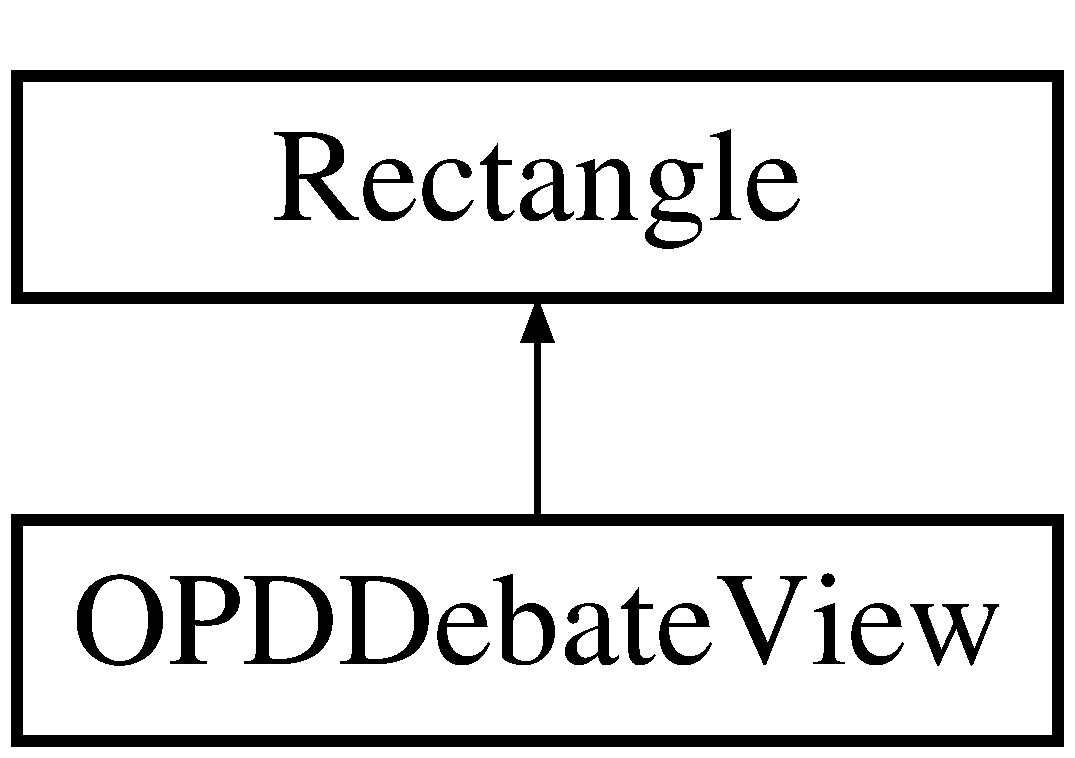
\includegraphics[height=2.000000cm]{classOPDDebateView}
\end{center}
\end{figure}
\subsection*{Signals}
\begin{DoxyCompactItemize}
\item 
\hypertarget{classOPDDebateView_a46391129857f2a878384174bbe30804d}{void \hyperlink{classOPDDebateView_a46391129857f2a878384174bbe30804d}{remove} ()}\label{classOPDDebateView_a46391129857f2a878384174bbe30804d}

\begin{DoxyCompactList}\small\item\em Called when the user indicates that the diplayed debate should be removed. \end{DoxyCompactList}\end{DoxyCompactItemize}
\subsection*{Properties}
\begin{DoxyCompactItemize}
\item 
\hypertarget{classOPDDebateView_abe79925c1c6e2c9cf8ed5bbdb37e5754}{bool \hyperlink{classOPDDebateView_abe79925c1c6e2c9cf8ed5bbdb37e5754}{editable}}\label{classOPDDebateView_abe79925c1c6e2c9cf8ed5bbdb37e5754}

\begin{DoxyCompactList}\small\item\em Holds if the number of speakers can be edited. \end{DoxyCompactList}\item 
\hypertarget{classOPDDebateView_a86367cec3e13cad756ffaccae8aa6aab}{O\-P\-D\-Debate \hyperlink{classOPDDebateView_a86367cec3e13cad756ffaccae8aa6aab}{op\-Debate}}\label{classOPDDebateView_a86367cec3e13cad756ffaccae8aa6aab}

\begin{DoxyCompactList}\small\item\em The underlying data model. \end{DoxyCompactList}\item 
\hypertarget{classOPDDebateView_a51f818917bd4c385d65fbfe1f83317e3}{\hyperlink{classSeatToSpeakerMapper}{Seat\-To\-Speaker\-Mapper} \hyperlink{classOPDDebateView_a51f818917bd4c385d65fbfe1f83317e3}{mapper}}\label{classOPDDebateView_a51f818917bd4c385d65fbfe1f83317e3}

\begin{DoxyCompactList}\small\item\em Maps positions to speaker names. The names will be displayed next to the speakers. \end{DoxyCompactList}\end{DoxyCompactItemize}


\subsection{Detailed Description}
Displays an O\-P debate. 

Allows editing the number of speakers participating in the debate. 

The documentation for this class was generated from the following file\-:\begin{DoxyCompactItemize}
\item 
/home/stoef/qt/projects/ddt/ddt/qml/ddt/O\-P\-D\-Debate\-View.\-qml\end{DoxyCompactItemize}

\hypertarget{classOPDebate}{\section{O\-P\-Debate Class Reference}
\label{classOPDebate}\index{O\-P\-Debate@{O\-P\-Debate}}
}


Represents a debate in O\-P\-D-\/format.  




{\ttfamily \#include $<$opdebate.\-h$>$}

Inheritance diagram for O\-P\-Debate\-:\begin{figure}[H]
\begin{center}
\leavevmode
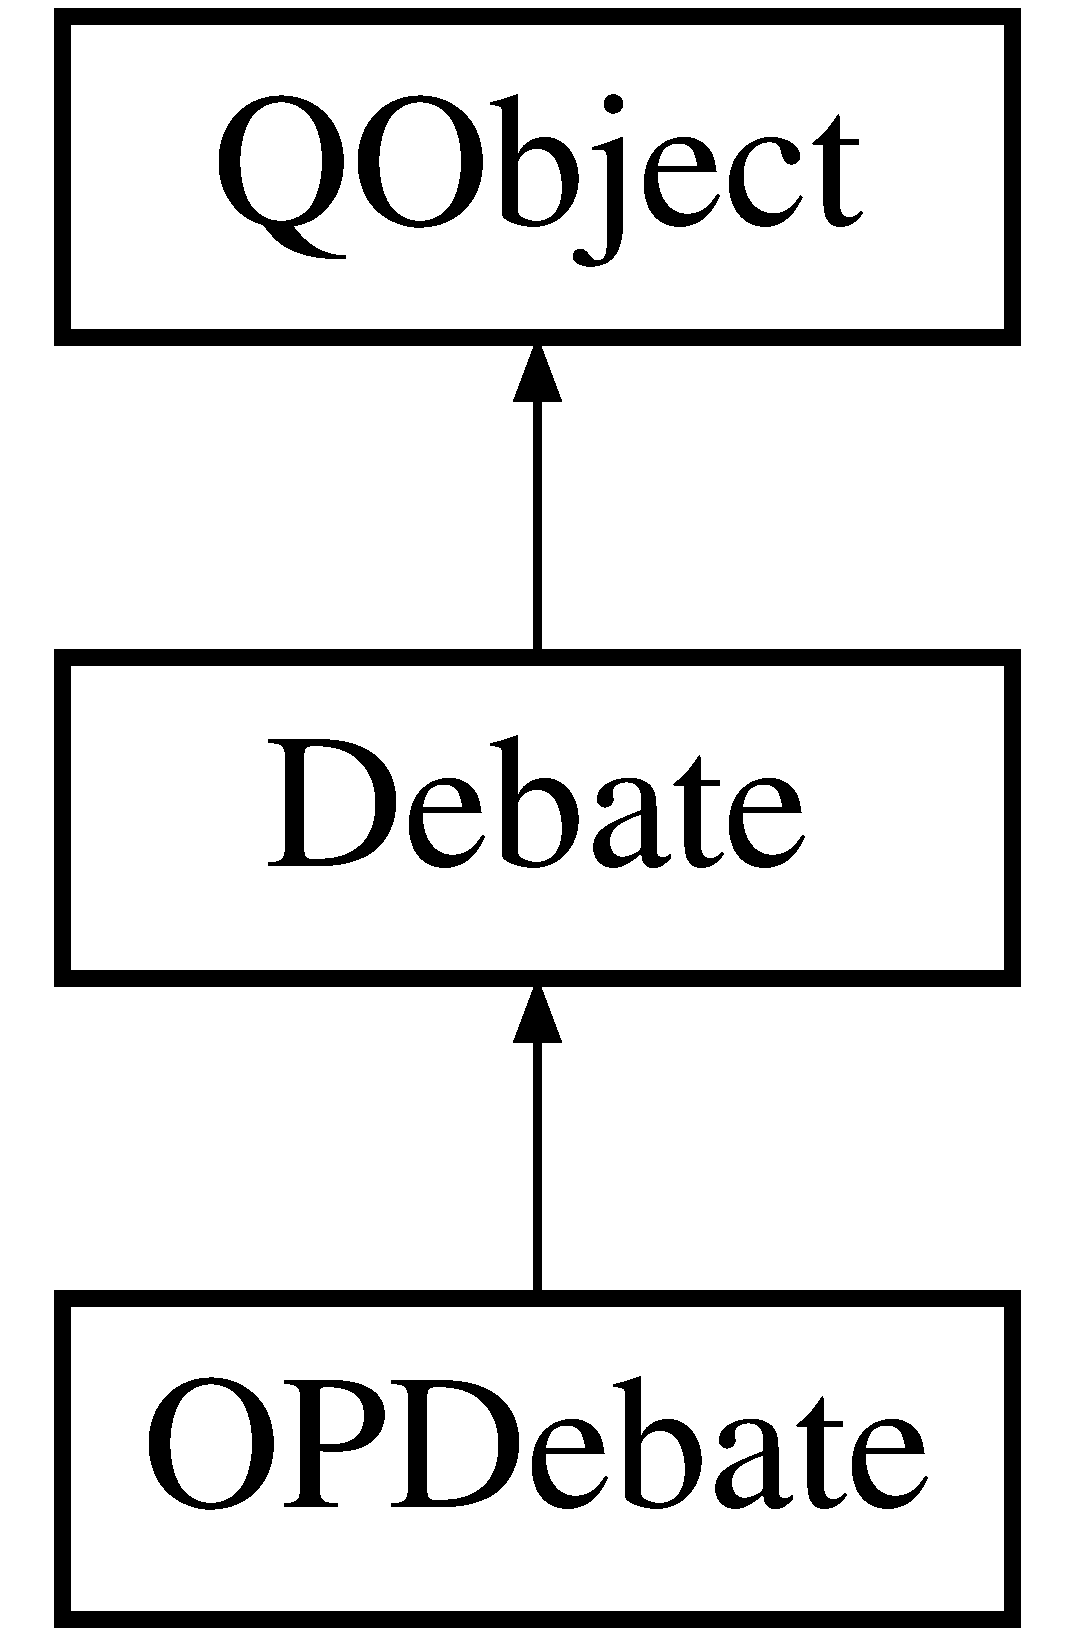
\includegraphics[height=3.000000cm]{classOPDebate}
\end{center}
\end{figure}
\subsection*{Signals}
\begin{DoxyCompactItemize}
\item 
\hypertarget{classOPDebate_a6c83bee3407b751c774280196ccace02}{void {\bfseries gov\-Places\-Changed} ()}\label{classOPDebate_a6c83bee3407b751c774280196ccace02}

\item 
\hypertarget{classOPDebate_a13cb748ff7ab86227f580013425565d7}{void {\bfseries op\-Places\-Changed} ()}\label{classOPDebate_a13cb748ff7ab86227f580013425565d7}

\item 
\hypertarget{classOPDebate_a9ec85e8b2dd66bdf54b23012f625b6ed}{void {\bfseries ffr\-Places\-Changed} ()}\label{classOPDebate_a9ec85e8b2dd66bdf54b23012f625b6ed}

\end{DoxyCompactItemize}
\subsection*{Public Member Functions}
\begin{DoxyCompactItemize}
\item 
\hypertarget{classOPDebate_aab5adce4866e4dcb26559e48d6eda000}{{\bfseries O\-P\-Debate} (Q\-Object $\ast$parent=0)}\label{classOPDebate_aab5adce4866e4dcb26559e48d6eda000}

\item 
\hypertarget{classOPDebate_ae23419710ab432c88ff520f16eb4ac2e}{int {\bfseries gov\-Places} ()}\label{classOPDebate_ae23419710ab432c88ff520f16eb4ac2e}

\item 
\hypertarget{classOPDebate_a68438ede1c10f4c58d1126a67fff3830}{void {\bfseries set\-Gov\-Places} (int \hyperlink{classOPDebate_ab84df4cd7885bff2c1aba90cebfe2b16}{gov\-Places})}\label{classOPDebate_a68438ede1c10f4c58d1126a67fff3830}

\item 
\hypertarget{classOPDebate_a3c5dbd12883f161144a0e7949b88d29f}{int {\bfseries op\-Places} ()}\label{classOPDebate_a3c5dbd12883f161144a0e7949b88d29f}

\item 
\hypertarget{classOPDebate_a53083010036023ba32989a2f73d15f3c}{void {\bfseries set\-Op\-Places} (int \hyperlink{classOPDebate_ab957581d6e4ca6769ef88095f8245b70}{op\-Places})}\label{classOPDebate_a53083010036023ba32989a2f73d15f3c}

\item 
\hypertarget{classOPDebate_a175d53a41790796ccf213ba12bce2a92}{int {\bfseries ffr\-Places} ()}\label{classOPDebate_a175d53a41790796ccf213ba12bce2a92}

\item 
\hypertarget{classOPDebate_a0fb3598f3bced7ece35b776ed803bad4}{void {\bfseries set\-Ffr\-Places} (int \hyperlink{classOPDebate_a9c1bc648302a8c503fc8cc4893a1ac26}{ffr\-Places})}\label{classOPDebate_a0fb3598f3bced7ece35b776ed803bad4}

\item 
\hypertarget{classOPDebate_a770a195089587e670ec9b705ea26e86a}{const Q\-List$<$ \hyperlink{classDebate_ae9871a36a2f3de7a7da8922d70fbece4}{Role\-Group} $>$ $\ast$ \hyperlink{classOPDebate_a770a195089587e670ec9b705ea26e86a}{get\-Roles\-For\-Debate} ()}\label{classOPDebate_a770a195089587e670ec9b705ea26e86a}

\begin{DoxyCompactList}\small\item\em Returns all roles that belong to this debate. \end{DoxyCompactList}\item 
\hypertarget{classOPDebate_a6bf6a7dcb35ed62f5289696259c5fcdd}{\hyperlink{classDebate_a537fac343de1edd412012e4180b52e04}{Debate\-Format} {\bfseries format} ()}\label{classOPDebate_a6bf6a7dcb35ed62f5289696259c5fcdd}

\item 
\hypertarget{classOPDebate_aed14a9f7d9019fe304af5811c28592e0}{int {\bfseries num\-Places} ()}\label{classOPDebate_aed14a9f7d9019fe304af5811c28592e0}

\end{DoxyCompactItemize}
\subsection*{Properties}
\begin{DoxyCompactItemize}
\item 
\hypertarget{classOPDebate_ab84df4cd7885bff2c1aba90cebfe2b16}{int \hyperlink{classOPDebate_ab84df4cd7885bff2c1aba90cebfe2b16}{gov\-Places}}\label{classOPDebate_ab84df4cd7885bff2c1aba90cebfe2b16}

\begin{DoxyCompactList}\small\item\em Holds the number of places on the government side. \end{DoxyCompactList}\item 
\hypertarget{classOPDebate_ab957581d6e4ca6769ef88095f8245b70}{int \hyperlink{classOPDebate_ab957581d6e4ca6769ef88095f8245b70}{op\-Places}}\label{classOPDebate_ab957581d6e4ca6769ef88095f8245b70}

\begin{DoxyCompactList}\small\item\em Holds the number of places on the opposition side. \end{DoxyCompactList}\item 
\hypertarget{classOPDebate_a9c1bc648302a8c503fc8cc4893a1ac26}{int \hyperlink{classOPDebate_a9c1bc648302a8c503fc8cc4893a1ac26}{ffr\-Places}}\label{classOPDebate_a9c1bc648302a8c503fc8cc4893a1ac26}

\begin{DoxyCompactList}\small\item\em Holds the number of F\-F\-Rs. \end{DoxyCompactList}\end{DoxyCompactItemize}
\subsection*{Additional Inherited Members}


\subsection{Detailed Description}
Represents a debate in O\-P\-D-\/format. 

O\-P\-D (Offene Parlamentarische Debatte) is a popular German format for debating. The debate has 3 different roles, the government, the opposition and the F\-F\-R (Fraktionsfreie Redner). Each role consists of 3 speakers. The debate is judicated by at least one judicator.

This class allows the representation of understaffed debates with less than 3 speakers in a speaker role or no judicator. \begin{DoxySeeAlso}{See Also}
\hyperlink{classDebate}{Debate} \hyperlink{classBPSDebate}{B\-P\-S\-Debate} 
\end{DoxySeeAlso}


The documentation for this class was generated from the following files\-:\begin{DoxyCompactItemize}
\item 
/home/stoef/qt/projects/ddt/ddt/src/opdebate.\-h\item 
/home/stoef/qt/projects/ddt/ddt/src/opdebate.\-cpp\end{DoxyCompactItemize}

\hypertarget{classPrototypeQListQmlWrapper}{\section{Prototype\-Q\-List\-Qml\-Wrapper Class Reference}
\label{classPrototypeQListQmlWrapper}\index{Prototype\-Q\-List\-Qml\-Wrapper@{Prototype\-Q\-List\-Qml\-Wrapper}}
}


A \hyperlink{classQListQmlWrapper}{Q\-List\-Qml\-Wrapper} with roles extrated from a prototype object.  




{\ttfamily \#include $<$prototypeqlistqmlwrapper.\-h$>$}

Inheritance diagram for Prototype\-Q\-List\-Qml\-Wrapper\-:\begin{figure}[H]
\begin{center}
\leavevmode
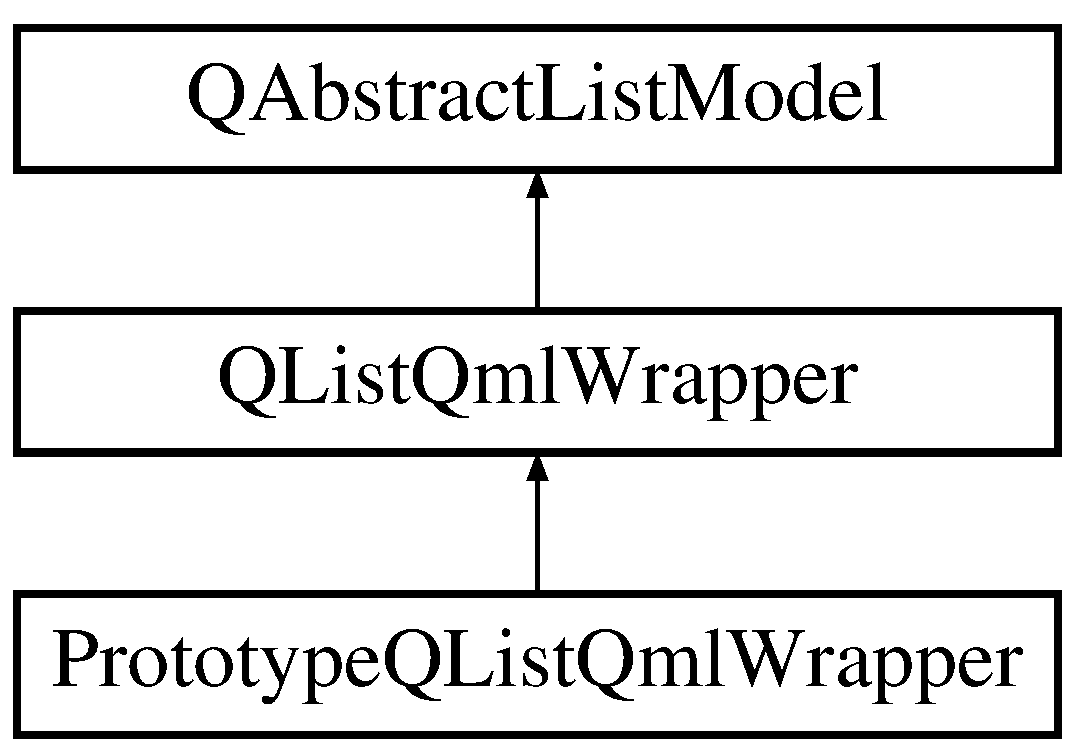
\includegraphics[height=3.000000cm]{classPrototypeQListQmlWrapper}
\end{center}
\end{figure}
\subsection*{Public Member Functions}
\begin{DoxyCompactItemize}
\item 
\hyperlink{classPrototypeQListQmlWrapper_aa57c170d4bc111a8d0e3fb029d9aee07}{Prototype\-Q\-List\-Qml\-Wrapper} (const Q\-Object $\ast$prototype, Q\-Object $\ast$parent=0)
\begin{DoxyCompactList}\small\item\em Creates a new {\ttfamily \hyperlink{classPrototypeQListQmlWrapper}{Prototype\-Q\-List\-Qml\-Wrapper}} with a given prototype. The objects role\-Names are read from the prototype's properties. \end{DoxyCompactList}\item 
\hypertarget{classPrototypeQListQmlWrapper_aebafcec43fe90b0913b05def79db52fb}{Q\-Hash$<$ int, Q\-Byte\-Array $>$ {\bfseries role\-Names} () const }\label{classPrototypeQListQmlWrapper_aebafcec43fe90b0913b05def79db52fb}

\end{DoxyCompactItemize}
\subsection*{Additional Inherited Members}


\subsection{Detailed Description}
A \hyperlink{classQListQmlWrapper}{Q\-List\-Qml\-Wrapper} with roles extrated from a prototype object. 

\hyperlink{classQListQmlWrapper}{Q\-List\-Qml\-Wrapper} cannot be used without specifying its role\-Names. {\ttfamily \hyperlink{classPrototypeQListQmlWrapper}{Prototype\-Q\-List\-Qml\-Wrapper}} inherits \hyperlink{classQListQmlWrapper}{Q\-List\-Qml\-Wrapper} and redefines {\ttfamily role\-Names}, the role names are obtained by reading all properties of a given prototype object. For each property 

\subsection{Constructor \& Destructor Documentation}
\hypertarget{classPrototypeQListQmlWrapper_aa57c170d4bc111a8d0e3fb029d9aee07}{\index{Prototype\-Q\-List\-Qml\-Wrapper@{Prototype\-Q\-List\-Qml\-Wrapper}!Prototype\-Q\-List\-Qml\-Wrapper@{Prototype\-Q\-List\-Qml\-Wrapper}}
\index{Prototype\-Q\-List\-Qml\-Wrapper@{Prototype\-Q\-List\-Qml\-Wrapper}!PrototypeQListQmlWrapper@{Prototype\-Q\-List\-Qml\-Wrapper}}
\subsubsection[{Prototype\-Q\-List\-Qml\-Wrapper}]{\setlength{\rightskip}{0pt plus 5cm}Prototype\-Q\-List\-Qml\-Wrapper\-::\-Prototype\-Q\-List\-Qml\-Wrapper (
\begin{DoxyParamCaption}
\item[{const Q\-Object $\ast$}]{prototype, }
\item[{Q\-Object $\ast$}]{parent = {\ttfamily 0}}
\end{DoxyParamCaption}
)}}\label{classPrototypeQListQmlWrapper_aa57c170d4bc111a8d0e3fb029d9aee07}


Creates a new {\ttfamily \hyperlink{classPrototypeQListQmlWrapper}{Prototype\-Q\-List\-Qml\-Wrapper}} with a given prototype. The objects role\-Names are read from the prototype's properties. 


\begin{DoxyParams}{Parameters}
{\em prototype} & an arbitrary object \\
\hline
{\em parent} & the object's parent \\
\hline
\end{DoxyParams}


The documentation for this class was generated from the following files\-:\begin{DoxyCompactItemize}
\item 
/home/stoef/qt/projects/ddt/ddt/src/prototypeqlistqmlwrapper.\-h\item 
/home/stoef/qt/projects/ddt/ddt/src/prototypeqlistqmlwrapper.\-cpp\end{DoxyCompactItemize}

\hypertarget{classQListQmlWrapper}{\section{Q\-List\-Qml\-Wrapper Class Reference}
\label{classQListQmlWrapper}\index{Q\-List\-Qml\-Wrapper@{Q\-List\-Qml\-Wrapper}}
}


Allows accessing a cpp list in Q\-M\-L.  




{\ttfamily \#include $<$qlistqmlwrapper.\-h$>$}

Inheritance diagram for Q\-List\-Qml\-Wrapper\-:\begin{figure}[H]
\begin{center}
\leavevmode
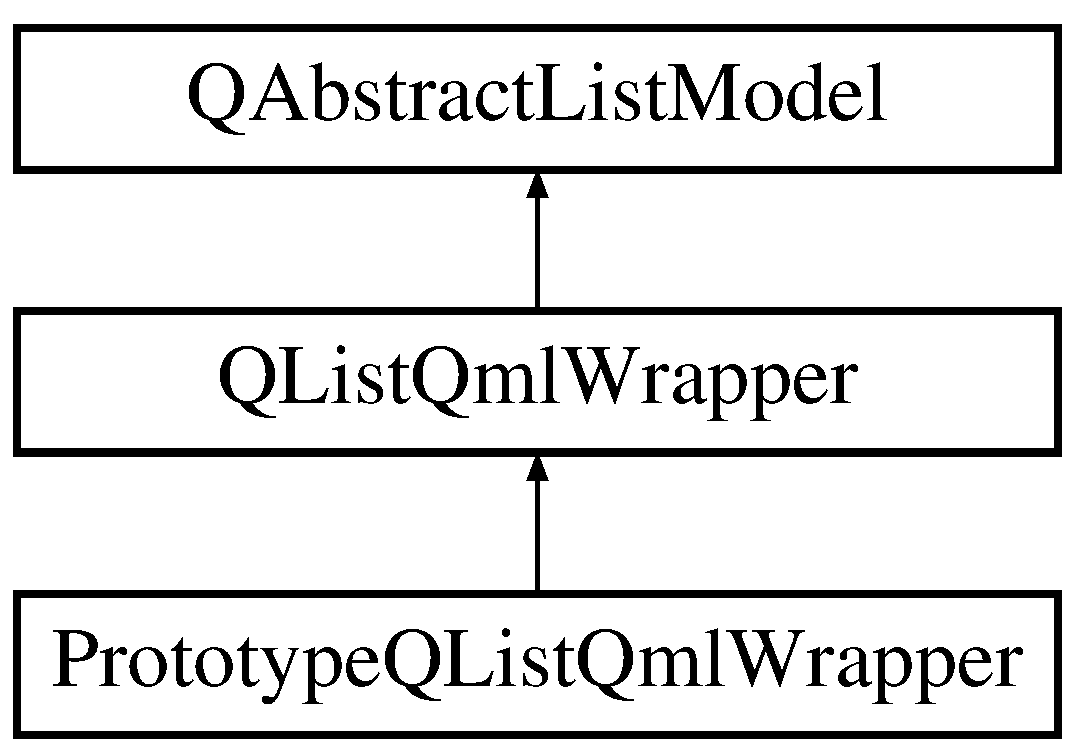
\includegraphics[height=3.000000cm]{classQListQmlWrapper}
\end{center}
\end{figure}
\subsection*{Public Slots}
\begin{DoxyCompactItemize}
\item 
Q\-\_\-\-I\-N\-V\-O\-K\-A\-B\-L\-E bool \hyperlink{classQListQmlWrapper_a08ee51fb27c3c6e6c21685cec176dfe0}{remove} (Q\-Object $\ast$object)
\end{DoxyCompactItemize}
\subsection*{Signals}
\begin{DoxyCompactItemize}
\item 
void \hyperlink{classQListQmlWrapper_a098f245657e03039eb01ef586dba9b5e}{list\-Changed} ()
\item 
\hypertarget{classQListQmlWrapper_a926184c29000446a6f4301a5fc57de4e}{void {\bfseries row\-Count\-Changed} ()}\label{classQListQmlWrapper_a926184c29000446a6f4301a5fc57de4e}

\end{DoxyCompactItemize}
\subsection*{Public Member Functions}
\begin{DoxyCompactItemize}
\item 
\hyperlink{classQListQmlWrapper_aeef385347fe1fc0c299f26046652a56c}{Q\-List\-Qml\-Wrapper} (Q\-Object $\ast$parent=0)
\begin{DoxyCompactList}\small\item\em Creates a new \hyperlink{classQListQmlWrapper}{Q\-List\-Qml\-Wrapper} with a given parent. \end{DoxyCompactList}\item 
\hypertarget{classQListQmlWrapper_ad6bb3bc6cf1044720c77962ed3d028e2}{Q\-Variant {\bfseries data} (const Q\-Model\-Index \&index, int role) const }\label{classQListQmlWrapper_ad6bb3bc6cf1044720c77962ed3d028e2}

\item 
\hypertarget{classQListQmlWrapper_a9ecb0a6b14f74c75e5d871542a07c8ba}{bool {\bfseries set\-Data} (const Q\-Model\-Index \&index, const Q\-Variant \&value, int role)}\label{classQListQmlWrapper_a9ecb0a6b14f74c75e5d871542a07c8ba}

\item 
\hypertarget{classQListQmlWrapper_a38d2b1788b6943874cdc465dc437331c}{virtual Q\-Hash$<$ int, Q\-Byte\-Array $>$ {\bfseries role\-Names} () const }\label{classQListQmlWrapper_a38d2b1788b6943874cdc465dc437331c}

\item 
\hypertarget{classQListQmlWrapper_a382a39110f33537bff9f49d7c0fd4fdf}{Qt\-::\-Item\-Flags {\bfseries flags} (const Q\-Model\-Index \&index) const }\label{classQListQmlWrapper_a382a39110f33537bff9f49d7c0fd4fdf}

\item 
\hypertarget{classQListQmlWrapper_a156c45b9f122fea8394ec821f47c41fe}{int {\bfseries row\-Count} (const Q\-Model\-Index \&parent=Q\-Model\-Index()) const }\label{classQListQmlWrapper_a156c45b9f122fea8394ec821f47c41fe}

\item 
\hypertarget{classQListQmlWrapper_a78ba996cd2cff329e8cb6081e986b056}{Q\-\_\-\-I\-N\-V\-O\-K\-A\-B\-L\-E void \hyperlink{classQListQmlWrapper_a78ba996cd2cff329e8cb6081e986b056}{append\-Row} (Q\-Object $\ast$item)}\label{classQListQmlWrapper_a78ba996cd2cff329e8cb6081e986b056}

\begin{DoxyCompactList}\small\item\em Appends an item to the wrapper's list. \end{DoxyCompactList}\item 
\hypertarget{classQListQmlWrapper_ae580eaadaa6abb6f5f9ca6bbb5b91fa6}{void \hyperlink{classQListQmlWrapper_ae580eaadaa6abb6f5f9ca6bbb5b91fa6}{append\-Rows} (const Q\-List$<$ Q\-Object $\ast$ $>$ \&items)}\label{classQListQmlWrapper_ae580eaadaa6abb6f5f9ca6bbb5b91fa6}

\begin{DoxyCompactList}\small\item\em Appends multiple item's to the wrapper's list. \end{DoxyCompactList}\item 
\hypertarget{classQListQmlWrapper_a3e433fd322140e50f6de31d786fd1e90}{Q\-\_\-\-I\-N\-V\-O\-K\-A\-B\-L\-E void \hyperlink{classQListQmlWrapper_a3e433fd322140e50f6de31d786fd1e90}{insert\-Row} (int row, Q\-Object $\ast$item)}\label{classQListQmlWrapper_a3e433fd322140e50f6de31d786fd1e90}

\begin{DoxyCompactList}\small\item\em Inserts an item at a specific position. \end{DoxyCompactList}\item 
Q\-\_\-\-I\-N\-V\-O\-K\-A\-B\-L\-E bool \hyperlink{classQListQmlWrapper_ab23231912af75b767ed96a5061c18810}{remove\-Row} (int row, const Q\-Model\-Index \&parent=Q\-Model\-Index())
\item 
\hypertarget{classQListQmlWrapper_a2daa2ca530b342bd493928a4cf99eb22}{Q\-\_\-\-I\-N\-V\-O\-K\-A\-B\-L\-E bool \hyperlink{classQListQmlWrapper_a2daa2ca530b342bd493928a4cf99eb22}{remove\-Rows} (int row, int count, const Q\-Model\-Index \&parent=Q\-Model\-Index())}\label{classQListQmlWrapper_a2daa2ca530b342bd493928a4cf99eb22}

\begin{DoxyCompactList}\small\item\em Removes {\ttfamily count} items, starting from index {\ttfamily row} . \end{DoxyCompactList}\item 
\hypertarget{classQListQmlWrapper_a7baf8a6a8a3232a227423ddae0cd261b}{Q\-\_\-\-I\-N\-V\-O\-K\-A\-B\-L\-E Q\-Object $\ast$ \hyperlink{classQListQmlWrapper_a7baf8a6a8a3232a227423ddae0cd261b}{take\-Row} (int row)}\label{classQListQmlWrapper_a7baf8a6a8a3232a227423ddae0cd261b}

\begin{DoxyCompactList}\small\item\em Removes and returns an item at position {\ttfamily row} . \end{DoxyCompactList}\item 
\hypertarget{classQListQmlWrapper_a3ec0f6232df2dfee1eb2e2334efc76aa}{Q\-\_\-\-I\-N\-V\-O\-K\-A\-B\-L\-E void \hyperlink{classQListQmlWrapper_a3ec0f6232df2dfee1eb2e2334efc76aa}{clear} ()}\label{classQListQmlWrapper_a3ec0f6232df2dfee1eb2e2334efc76aa}

\begin{DoxyCompactList}\small\item\em Removes all roles. \end{DoxyCompactList}\item 
\hypertarget{classQListQmlWrapper_a6d3cd7291fa7b1d79b6bd488dc549e4f}{Q\-\_\-\-I\-N\-V\-O\-K\-A\-B\-L\-E bool \hyperlink{classQListQmlWrapper_a6d3cd7291fa7b1d79b6bd488dc549e4f}{contains} (Q\-Object $\ast$object)}\label{classQListQmlWrapper_a6d3cd7291fa7b1d79b6bd488dc549e4f}

\begin{DoxyCompactList}\small\item\em Returns {\ttfamily true} if {\ttfamily object} is contained in the wrappers list. \end{DoxyCompactList}\item 
Q\-\_\-\-I\-N\-V\-O\-K\-A\-B\-L\-E int \hyperlink{classQListQmlWrapper_a9430d2a06f3ee285538717f874d9f876}{index\-Of} (Q\-Object $\ast$object)
\item 
\hypertarget{classQListQmlWrapper_a473a63842191ef808dc8e5c1047f9f8f}{Q\-\_\-\-I\-N\-V\-O\-K\-A\-B\-L\-E Q\-Object $\ast$ \hyperlink{classQListQmlWrapper_a473a63842191ef808dc8e5c1047f9f8f}{get\-Row} (int row) const }\label{classQListQmlWrapper_a473a63842191ef808dc8e5c1047f9f8f}

\begin{DoxyCompactList}\small\item\em Returns the row at a given position. \end{DoxyCompactList}\item 
\hypertarget{classQListQmlWrapper_a4f476937745f5cb9cdfc5a8849e820a8}{const Q\-List$<$ Q\-Object $\ast$ $>$ $\ast$ \hyperlink{classQListQmlWrapper_a4f476937745f5cb9cdfc5a8849e820a8}{list} ()}\label{classQListQmlWrapper_a4f476937745f5cb9cdfc5a8849e820a8}

\begin{DoxyCompactList}\small\item\em Returns the list represented by this wrapper. \end{DoxyCompactList}\end{DoxyCompactItemize}
\subsection*{Properties}
\begin{DoxyCompactItemize}
\item 
\hypertarget{classQListQmlWrapper_a3aaa4cbf86d838af871a98d96fcbfe52}{int \hyperlink{classQListQmlWrapper_a3aaa4cbf86d838af871a98d96fcbfe52}{row\-Count}}\label{classQListQmlWrapper_a3aaa4cbf86d838af871a98d96fcbfe52}

\begin{DoxyCompactList}\small\item\em Holds the wrapper's number of items. \end{DoxyCompactList}\end{DoxyCompactItemize}


\subsection{Detailed Description}
Allows accessing a cpp list in Q\-M\-L. 

Q\-M\-L cannot handle lists of type {\ttfamily Q\-List}. This class fills this gap by offering a list like interface on the cpp side while inheriting {\ttfamily Q\-Abstract\-List\-Model}, which is neccessary for elements like the Q\-M\-L {\ttfamily List\-View}. A \hyperlink{classQListQmlWrapper}{Q\-List\-Qml\-Wrapper} can be set directly as a List\-View's, model, the model item roles are specified by a concrete subclass of  . See role\-Names for details.\par
Deleting an item will automatically remove it from the wrapper's list. 

\subsection{Constructor \& Destructor Documentation}
\hypertarget{classQListQmlWrapper_aeef385347fe1fc0c299f26046652a56c}{\index{Q\-List\-Qml\-Wrapper@{Q\-List\-Qml\-Wrapper}!Q\-List\-Qml\-Wrapper@{Q\-List\-Qml\-Wrapper}}
\index{Q\-List\-Qml\-Wrapper@{Q\-List\-Qml\-Wrapper}!QListQmlWrapper@{Q\-List\-Qml\-Wrapper}}
\subsubsection[{Q\-List\-Qml\-Wrapper}]{\setlength{\rightskip}{0pt plus 5cm}Q\-List\-Qml\-Wrapper\-::\-Q\-List\-Qml\-Wrapper (
\begin{DoxyParamCaption}
\item[{Q\-Object $\ast$}]{parent = {\ttfamily 0}}
\end{DoxyParamCaption}
)\hspace{0.3cm}{\ttfamily [explicit]}}}\label{classQListQmlWrapper_aeef385347fe1fc0c299f26046652a56c}


Creates a new \hyperlink{classQListQmlWrapper}{Q\-List\-Qml\-Wrapper} with a given parent. 

The wrapper's list is initially empty. 
\begin{DoxyParams}{Parameters}
{\em parent} & the object's parent \\
\hline
\end{DoxyParams}


\subsection{Member Function Documentation}
\hypertarget{classQListQmlWrapper_a9430d2a06f3ee285538717f874d9f876}{\index{Q\-List\-Qml\-Wrapper@{Q\-List\-Qml\-Wrapper}!index\-Of@{index\-Of}}
\index{index\-Of@{index\-Of}!QListQmlWrapper@{Q\-List\-Qml\-Wrapper}}
\subsubsection[{index\-Of}]{\setlength{\rightskip}{0pt plus 5cm}int Q\-List\-Qml\-Wrapper\-::index\-Of (
\begin{DoxyParamCaption}
\item[{Q\-Object $\ast$}]{object}
\end{DoxyParamCaption}
)}}\label{classQListQmlWrapper_a9430d2a06f3ee285538717f874d9f876}
Return the first occurence of a given object in the wrappers list. Returns -\/1 if the object is not contained. \hypertarget{classQListQmlWrapper_a098f245657e03039eb01ef586dba9b5e}{\index{Q\-List\-Qml\-Wrapper@{Q\-List\-Qml\-Wrapper}!list\-Changed@{list\-Changed}}
\index{list\-Changed@{list\-Changed}!QListQmlWrapper@{Q\-List\-Qml\-Wrapper}}
\subsubsection[{list\-Changed}]{\setlength{\rightskip}{0pt plus 5cm}void Q\-List\-Qml\-Wrapper\-::list\-Changed (
\begin{DoxyParamCaption}
{}
\end{DoxyParamCaption}
)\hspace{0.3cm}{\ttfamily [signal]}}}\label{classQListQmlWrapper_a098f245657e03039eb01ef586dba9b5e}
Emitted when items were added, moved or removed, or when an item's proeprty has changed. \hypertarget{classQListQmlWrapper_a08ee51fb27c3c6e6c21685cec176dfe0}{\index{Q\-List\-Qml\-Wrapper@{Q\-List\-Qml\-Wrapper}!remove@{remove}}
\index{remove@{remove}!QListQmlWrapper@{Q\-List\-Qml\-Wrapper}}
\subsubsection[{remove}]{\setlength{\rightskip}{0pt plus 5cm}bool Q\-List\-Qml\-Wrapper\-::remove (
\begin{DoxyParamCaption}
\item[{Q\-Object $\ast$}]{object}
\end{DoxyParamCaption}
)\hspace{0.3cm}{\ttfamily [slot]}}}\label{classQListQmlWrapper_a08ee51fb27c3c6e6c21685cec176dfe0}
Removes one occurence of  from the list. Returns {\ttfamily true} if an occurence could be removed \hypertarget{classQListQmlWrapper_ab23231912af75b767ed96a5061c18810}{\index{Q\-List\-Qml\-Wrapper@{Q\-List\-Qml\-Wrapper}!remove\-Row@{remove\-Row}}
\index{remove\-Row@{remove\-Row}!QListQmlWrapper@{Q\-List\-Qml\-Wrapper}}
\subsubsection[{remove\-Row}]{\setlength{\rightskip}{0pt plus 5cm}bool Q\-List\-Qml\-Wrapper\-::remove\-Row (
\begin{DoxyParamCaption}
\item[{int}]{row, }
\item[{const Q\-Model\-Index \&}]{parent = {\ttfamily QModelIndex()}}
\end{DoxyParamCaption}
)}}\label{classQListQmlWrapper_ab23231912af75b767ed96a5061c18810}
Removes an item with a given index. \begin{DoxyReturn}{Returns}
{\ttfamily true} the given row index was valid and an item was removed. 
\end{DoxyReturn}


The documentation for this class was generated from the following files\-:\begin{DoxyCompactItemize}
\item 
/home/stoef/qt/projects/ddt/ddt/src/qlistqmlwrapper.\-h\item 
/home/stoef/qt/projects/ddt/ddt/src/qlistqmlwrapper.\-cpp\end{DoxyCompactItemize}

\hypertarget{classResultPage}{\section{Result\-Page Class Reference}
\label{classResultPage}\index{Result\-Page@{Result\-Page}}
}
Inheritance diagram for Result\-Page\-:\begin{figure}[H]
\begin{center}
\leavevmode
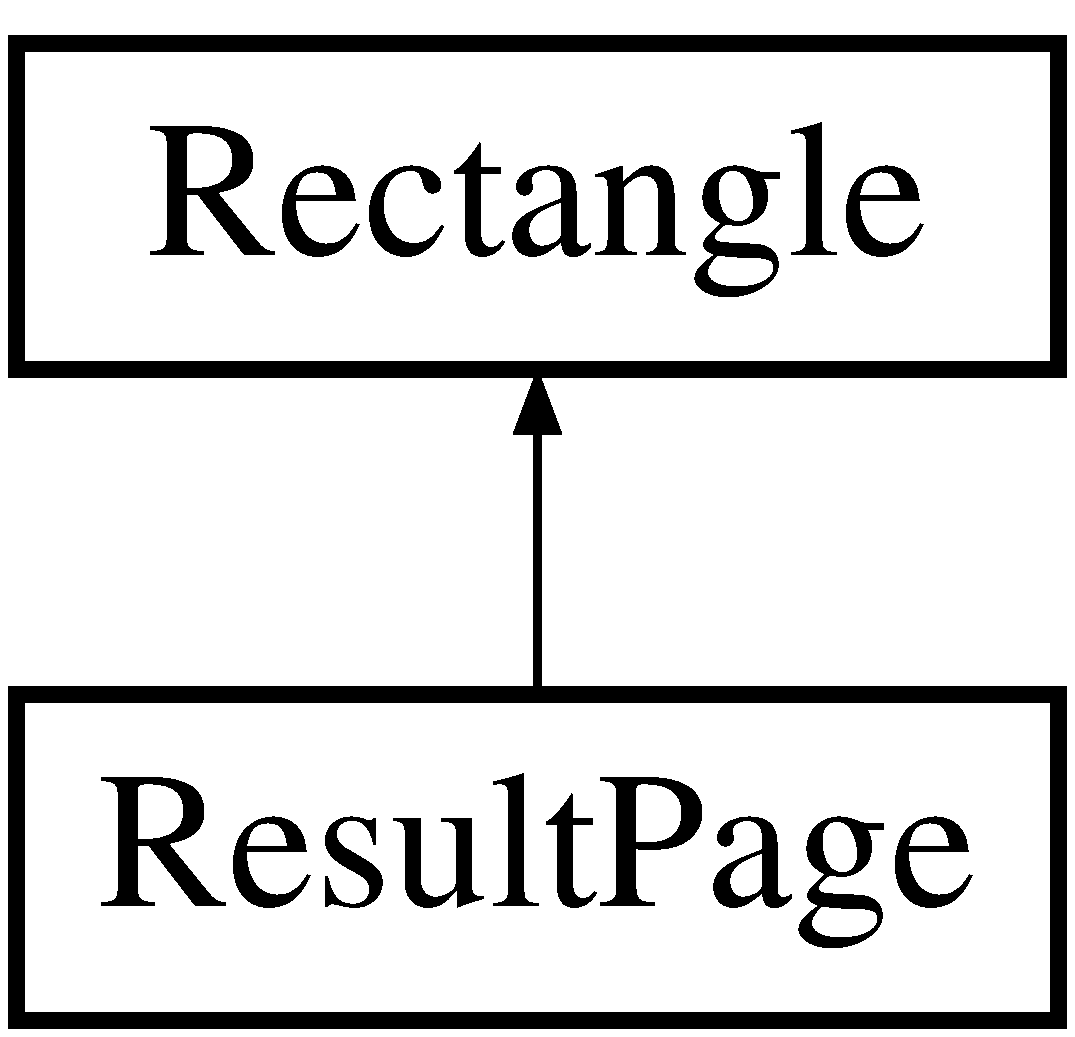
\includegraphics[height=2.000000cm]{classResultPage}
\end{center}
\end{figure}
\subsection*{Public Member Functions}
\begin{DoxyCompactItemize}
\item 
\hypertarget{classResultPage_af72c9a587fbec369997dd8a48ae22394}{void {\bfseries current\-Debate} ()}\label{classResultPage_af72c9a587fbec369997dd8a48ae22394}

\end{DoxyCompactItemize}
\subsection*{Properties}
\begin{DoxyCompactItemize}
\item 
\hypertarget{classResultPage_af42f22505361295fea95be9c24c2581b}{\hyperlink{classMainModel}{Main\-Model} \hyperlink{classResultPage_af42f22505361295fea95be9c24c2581b}{main\-Model}}\label{classResultPage_af42f22505361295fea95be9c24c2581b}

\begin{DoxyCompactList}\small\item\em The application's main model. \end{DoxyCompactList}\item 
int \hyperlink{classResultPage_ac6459fe5c02bd49ed488b428a1d9d766}{current\-Debate\-Index}
\item 
int \hyperlink{classResultPage_acfea637505034129528d4e4dcda06041}{current\-Solution\-Index}
\item 
Component \hyperlink{classResultPage_a4634d6af41a1cbf3f566b8dfa63ac67b}{tool\-Bar\-Component}
\item 
\hypertarget{classResultPage_a45726fea9e6169f39f19f5fe57edf614}{Action \hyperlink{classResultPage_a45726fea9e6169f39f19f5fe57edf614}{generate\-Solution\-Action}}\label{classResultPage_a45726fea9e6169f39f19f5fe57edf614}

\begin{DoxyCompactList}\small\item\em An action that starts the calculation of a new solution. \end{DoxyCompactList}\item 
\hypertarget{classResultPage_a48820af67f5ee61a4f2cd51040df269b}{Action \hyperlink{classResultPage_a48820af67f5ee61a4f2cd51040df269b}{interrupt\-Calculation\-Action}}\label{classResultPage_a48820af67f5ee61a4f2cd51040df269b}

\begin{DoxyCompactList}\small\item\em An action that interrupts the current calculation. \end{DoxyCompactList}\end{DoxyCompactItemize}


\subsection{Detailed Description}
Displays the results of a mapping process.

Shows the mapping between speakers and seats. Furthermore, the configuration of different rooms can be edited. 

\subsection{Property Documentation}
\hypertarget{classResultPage_ac6459fe5c02bd49ed488b428a1d9d766}{\index{Result\-Page@{Result\-Page}!current\-Debate\-Index@{current\-Debate\-Index}}
\index{current\-Debate\-Index@{current\-Debate\-Index}!ResultPage@{Result\-Page}}
\subsubsection[{current\-Debate\-Index}]{\setlength{\rightskip}{0pt plus 5cm}int Result\-Page\-::current\-Debate\-Index}}\label{classResultPage_ac6459fe5c02bd49ed488b428a1d9d766}
Specifies which debate is currently selected. \begin{DoxySeeAlso}{See Also}
\hyperlink{classMainModel_ab61e1b1925f4dc1ae94cdcafc579e3fe}{Main\-Model\-::debates} 
\end{DoxySeeAlso}
\hypertarget{classResultPage_acfea637505034129528d4e4dcda06041}{\index{Result\-Page@{Result\-Page}!current\-Solution\-Index@{current\-Solution\-Index}}
\index{current\-Solution\-Index@{current\-Solution\-Index}!ResultPage@{Result\-Page}}
\subsubsection[{current\-Solution\-Index}]{\setlength{\rightskip}{0pt plus 5cm}int Result\-Page\-::current\-Solution\-Index}}\label{classResultPage_acfea637505034129528d4e4dcda06041}
A {\ttfamily \hyperlink{classMainModel}{Main\-Model}} stores multiple precalculated solutions. This property specifies which solution is displayed. \hypertarget{classResultPage_a4634d6af41a1cbf3f566b8dfa63ac67b}{\index{Result\-Page@{Result\-Page}!tool\-Bar\-Component@{tool\-Bar\-Component}}
\index{tool\-Bar\-Component@{tool\-Bar\-Component}!ResultPage@{Result\-Page}}
\subsubsection[{tool\-Bar\-Component}]{\setlength{\rightskip}{0pt plus 5cm}Component Result\-Page\-::tool\-Bar\-Component}}\label{classResultPage_a4634d6af41a1cbf3f566b8dfa63ac67b}
A component containing control elements for this page. Should Be used in a {\ttfamily Tool\-Bar} 

The documentation for this class was generated from the following file\-:\begin{DoxyCompactItemize}
\item 
/home/stoef/qt/projects/ddt/ddt/qml/ddt/Result\-Page.\-qml\end{DoxyCompactItemize}

\hypertarget{structRoleLink}{\section{Role\-Link Struct Reference}
\label{structRoleLink}\index{Role\-Link@{Role\-Link}}
}
\subsection*{Public Attributes}
\begin{DoxyCompactItemize}
\item 
\hypertarget{structRoleLink_abcc31a77bf33b9efe7c5f48485c4d370}{\hyperlink{classDebate}{Debate} $\ast$ {\bfseries debate}}\label{structRoleLink_abcc31a77bf33b9efe7c5f48485c4d370}

\item 
\hypertarget{structRoleLink_ab9e7502c40c24b40d7a63dd534a739e4}{\hyperlink{classDebate_ae9871a36a2f3de7a7da8922d70fbece4}{Debate\-::\-Role\-Group} {\bfseries group}}\label{structRoleLink_ab9e7502c40c24b40d7a63dd534a739e4}

\item 
\hypertarget{structRoleLink_ae1cd0be803e73cab33405554db2ebc76}{int {\bfseries seat\-Index}}\label{structRoleLink_ae1cd0be803e73cab33405554db2ebc76}

\item 
\hypertarget{structRoleLink_af68987a39ab52ada8783cc27ef1d8f6f}{int {\bfseries seat\-Group\-Index}}\label{structRoleLink_af68987a39ab52ada8783cc27ef1d8f6f}

\item 
\hypertarget{structRoleLink_aaa7115d2c38c602e317435bdc81b1cd4}{bool {\bfseries has\-Speaker}}\label{structRoleLink_aaa7115d2c38c602e317435bdc81b1cd4}

\end{DoxyCompactItemize}


The documentation for this struct was generated from the following file\-:\begin{DoxyCompactItemize}
\item 
/home/stoef/qt/projects/ddt/ddt/src/matchingsolver.\-h\end{DoxyCompactItemize}

\hypertarget{classRoundButton}{\section{Round\-Button Class Reference}
\label{classRoundButton}\index{Round\-Button@{Round\-Button}}
}
Inheritance diagram for Round\-Button\-:\begin{figure}[H]
\begin{center}
\leavevmode
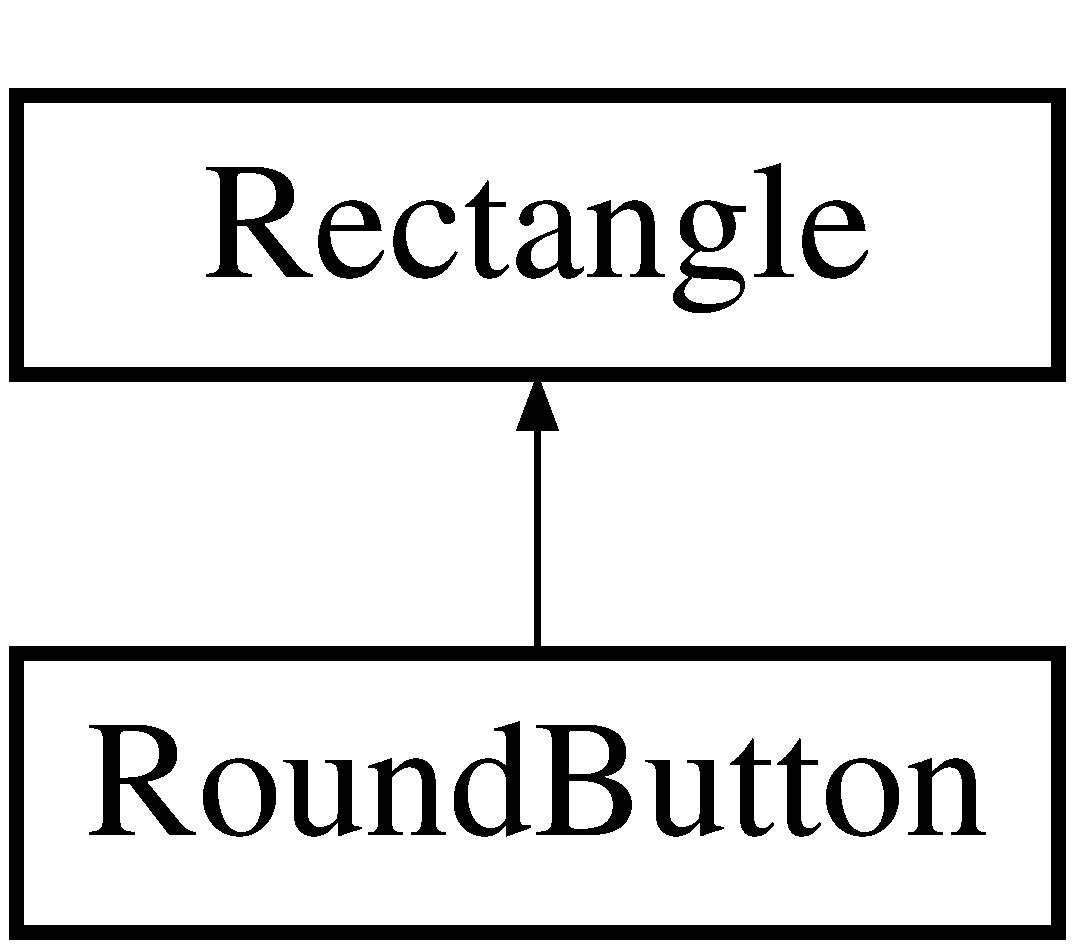
\includegraphics[height=2.000000cm]{classRoundButton}
\end{center}
\end{figure}
\subsection*{Signals}
\begin{DoxyCompactItemize}
\item 
\hypertarget{classRoundButton_a0b3ac16502895acc5a51d45aef7a19c2}{void \hyperlink{classRoundButton_a0b3ac16502895acc5a51d45aef7a19c2}{clicked} ()}\label{classRoundButton_a0b3ac16502895acc5a51d45aef7a19c2}

\begin{DoxyCompactList}\small\item\em called when the button is clicked \end{DoxyCompactList}\end{DoxyCompactItemize}
\subsection*{Properties}
\begin{DoxyCompactItemize}
\item 
\hypertarget{classRoundButton_a48b76509d0dabcddc89591eb0f3d1991}{alias \hyperlink{classRoundButton_a48b76509d0dabcddc89591eb0f3d1991}{text}}\label{classRoundButton_a48b76509d0dabcddc89591eb0f3d1991}

\begin{DoxyCompactList}\small\item\em text displayed on the button's surface \end{DoxyCompactList}\end{DoxyCompactItemize}


\subsection{Detailed Description}
A simple round button with gradient background and hover animation. 

The documentation for this class was generated from the following file\-:\begin{DoxyCompactItemize}
\item 
/home/stoef/qt/projects/ddt/ddt/qml/ddt/Round\-Button.\-qml\end{DoxyCompactItemize}

\hypertarget{classSeatToSpeakerMapper}{\section{Seat\-To\-Speaker\-Mapper Class Reference}
\label{classSeatToSpeakerMapper}\index{Seat\-To\-Speaker\-Mapper@{Seat\-To\-Speaker\-Mapper}}
}


Represents the results of a matching process.  




{\ttfamily \#include $<$seattospeakermapper.\-h$>$}

Inheritance diagram for Seat\-To\-Speaker\-Mapper\-:\begin{figure}[H]
\begin{center}
\leavevmode
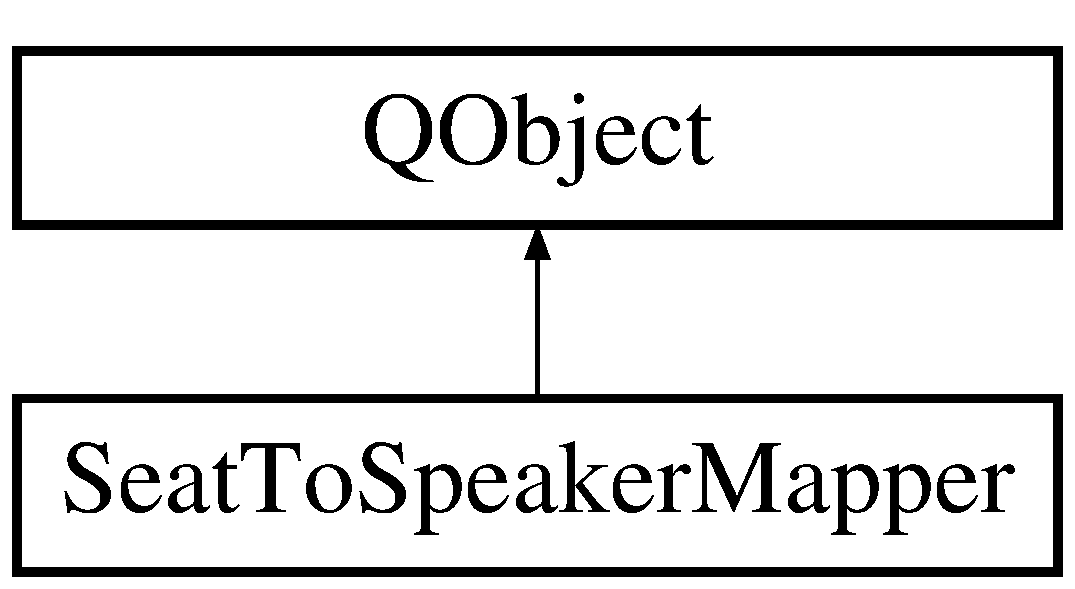
\includegraphics[height=2.000000cm]{classSeatToSpeakerMapper}
\end{center}
\end{figure}
\subsection*{Public Member Functions}
\begin{DoxyCompactItemize}
\item 
\hypertarget{classSeatToSpeakerMapper_a9978292542a75eef5da708caf487c76b}{\hyperlink{classSeatToSpeakerMapper_a9978292542a75eef5da708caf487c76b}{Seat\-To\-Speaker\-Mapper} (Q\-Object $\ast$parent=0)}\label{classSeatToSpeakerMapper_a9978292542a75eef5da708caf487c76b}

\begin{DoxyCompactList}\small\item\em Creates a new \hyperlink{classSeatToSpeakerMapper}{Seat\-To\-Speaker\-Mapper} with a given parent. \end{DoxyCompactList}\item 
void \hyperlink{classSeatToSpeakerMapper_afecf8db446d9e0adfe5a5d14bf28e232}{add\-Mapping} (\hyperlink{classDebate}{Debate} $\ast$debate, \hyperlink{classDebate_ae9871a36a2f3de7a7da8922d70fbece4}{Debate\-::\-Role\-Group} group, int seat\-Index, \hyperlink{classSpeakerModel}{Speaker\-Model} $\ast$speaker)
\begin{DoxyCompactList}\small\item\em Maps a speaker to a specific seat in a debate. \end{DoxyCompactList}\item 
\hyperlink{classTableNames}{Table\-Names} $\ast$ \hyperlink{classSeatToSpeakerMapper_a4664111c6684c4943173594ff631261a}{get\-Names\-For\-Table} (\hyperlink{classDebate}{Debate} $\ast$debate, \hyperlink{classDebate_ae9871a36a2f3de7a7da8922d70fbece4}{Debate\-::\-Role\-Group} group)
\begin{DoxyCompactList}\small\item\em Returns a {\ttfamily \hyperlink{classTableNames}{Table\-Names}} object representing the speakers at some table. \end{DoxyCompactList}\item 
\hypertarget{classSeatToSpeakerMapper_a900eeb6a8050ad64aa0ae1eea69bcc97}{Q\-\_\-\-I\-N\-V\-O\-K\-A\-B\-L\-E \hyperlink{classTableNames}{Table\-Names} $\ast$ {\bfseries get\-Names\-For\-Table} (\hyperlink{classDebate}{Debate} $\ast$debate, int group)}\label{classSeatToSpeakerMapper_a900eeb6a8050ad64aa0ae1eea69bcc97}

\end{DoxyCompactItemize}


\subsection{Detailed Description}
Represents the results of a matching process. 

{\ttfamily \hyperlink{classSeatToSpeakerMapper}{Seat\-To\-Speaker\-Mapper}} describes a mapping from different places in a debate to speakers that were mapped to these places. 

\subsection{Member Function Documentation}
\hypertarget{classSeatToSpeakerMapper_afecf8db446d9e0adfe5a5d14bf28e232}{\index{Seat\-To\-Speaker\-Mapper@{Seat\-To\-Speaker\-Mapper}!add\-Mapping@{add\-Mapping}}
\index{add\-Mapping@{add\-Mapping}!SeatToSpeakerMapper@{Seat\-To\-Speaker\-Mapper}}
\subsubsection[{add\-Mapping}]{\setlength{\rightskip}{0pt plus 5cm}void Seat\-To\-Speaker\-Mapper\-::add\-Mapping (
\begin{DoxyParamCaption}
\item[{{\bf Debate} $\ast$}]{debate, }
\item[{{\bf Debate\-::\-Role\-Group}}]{group, }
\item[{int}]{seat\-Index, }
\item[{{\bf Speaker\-Model} $\ast$}]{speaker}
\end{DoxyParamCaption}
)}}\label{classSeatToSpeakerMapper_afecf8db446d9e0adfe5a5d14bf28e232}


Maps a speaker to a specific seat in a debate. 


\begin{DoxyParams}{Parameters}
{\em debate} & the debate in which the speaker is seated \\
\hline
{\em group} & the role to which the speaker was mapped \\
\hline
{\em seat\-Index} & the speaker's position at his table \\
\hline
{\em speaker} & a speaker that is mapped to a given seat \\
\hline
\end{DoxyParams}
\hypertarget{classSeatToSpeakerMapper_a4664111c6684c4943173594ff631261a}{\index{Seat\-To\-Speaker\-Mapper@{Seat\-To\-Speaker\-Mapper}!get\-Names\-For\-Table@{get\-Names\-For\-Table}}
\index{get\-Names\-For\-Table@{get\-Names\-For\-Table}!SeatToSpeakerMapper@{Seat\-To\-Speaker\-Mapper}}
\subsubsection[{get\-Names\-For\-Table}]{\setlength{\rightskip}{0pt plus 5cm}{\bf Table\-Names} $\ast$ Seat\-To\-Speaker\-Mapper\-::get\-Names\-For\-Table (
\begin{DoxyParamCaption}
\item[{{\bf Debate} $\ast$}]{debate, }
\item[{{\bf Debate\-::\-Role\-Group}}]{group}
\end{DoxyParamCaption}
)}}\label{classSeatToSpeakerMapper_a4664111c6684c4943173594ff631261a}


Returns a {\ttfamily \hyperlink{classTableNames}{Table\-Names}} object representing the speakers at some table. 


\begin{DoxyParams}{Parameters}
{\em debate} & the debate where the table is placed \\
\hline
{\em group} & the role group to which the table belongs to \\
\hline
\end{DoxyParams}
\begin{DoxyReturn}{Returns}
A {\ttfamily \hyperlink{classTableNames}{Table\-Names}} object representing a table. 
\end{DoxyReturn}


The documentation for this class was generated from the following files\-:\begin{DoxyCompactItemize}
\item 
/home/stoef/qt/projects/ddt/ddt/src/seattospeakermapper.\-h\item 
/home/stoef/qt/projects/ddt/ddt/src/seattospeakermapper.\-cpp\end{DoxyCompactItemize}

\hypertarget{classSpeakerList}{\section{Speaker\-List Class Reference}
\label{classSpeakerList}\index{Speaker\-List@{Speaker\-List}}
}
Inheritance diagram for Speaker\-List\-:\begin{figure}[H]
\begin{center}
\leavevmode
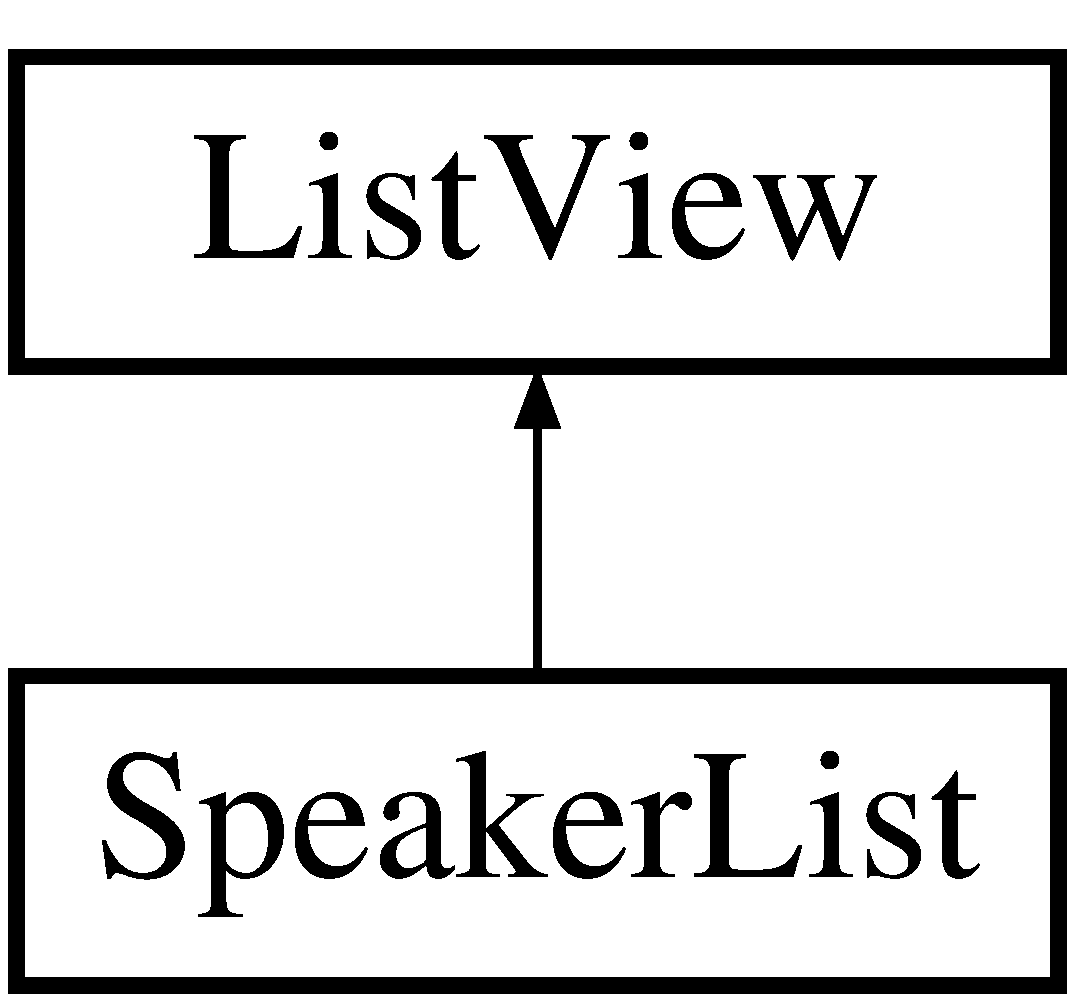
\includegraphics[height=2.000000cm]{classSpeakerList}
\end{center}
\end{figure}
\subsection*{Public Member Functions}
\begin{DoxyCompactItemize}
\item 
\hypertarget{classSpeakerList_acc93fae1ea562472a8786779a468b1a7}{void {\bfseries clear\-Selection} ()}\label{classSpeakerList_acc93fae1ea562472a8786779a468b1a7}

\item 
\hypertarget{classSpeakerList_accdfc9a4a5618a4cdf1542aff03b2951}{void {\bfseries add\-Between\-To\-Selection} (a, b)}\label{classSpeakerList_accdfc9a4a5618a4cdf1542aff03b2951}

\item 
\hypertarget{classSpeakerList_ab09c25267d412ccae58cf307b778cba8}{void {\bfseries toggle\-Selection} (index)}\label{classSpeakerList_ab09c25267d412ccae58cf307b778cba8}

\item 
\hypertarget{classSpeakerList_aa52606d08ffd7d4b3a8420f29b234b77}{void {\bfseries add\-To\-Selection} (index)}\label{classSpeakerList_aa52606d08ffd7d4b3a8420f29b234b77}

\item 
\hypertarget{classSpeakerList_aa8b9882f352863ddcf4fb9679decb30e}{void {\bfseries selection\-Contains} (index)}\label{classSpeakerList_aa8b9882f352863ddcf4fb9679decb30e}

\item 
\hypertarget{classSpeakerList_a153cb3c5302699333d0b9f55c877b985}{void {\bfseries remove\-From\-Selection} (index)}\label{classSpeakerList_a153cb3c5302699333d0b9f55c877b985}

\item 
\hypertarget{classSpeakerList_a53fdfda0940f37c71bad8c5a050df4dc}{void {\bfseries select\-Current\-Element} (event, force\-Focus)}\label{classSpeakerList_a53fdfda0940f37c71bad8c5a050df4dc}

\item 
\hypertarget{classSpeakerList_a515bd2b87e3fe64dc44f75f07366ba69}{void {\bfseries selection\-Event} (mouse, index, delegate)}\label{classSpeakerList_a515bd2b87e3fe64dc44f75f07366ba69}

\end{DoxyCompactItemize}
\subsection*{Properties}
\begin{DoxyCompactItemize}
\item 
\hypertarget{classSpeakerList_a3e4892babaaccd9db11118c2e3549f92}{\hyperlink{classMainModel}{Main\-Model} \hyperlink{classSpeakerList_a3e4892babaaccd9db11118c2e3549f92}{main\-Model}}\label{classSpeakerList_a3e4892babaaccd9db11118c2e3549f92}

\begin{DoxyCompactList}\small\item\em The applications {\ttfamily \hyperlink{classMainModel}{Main\-Model}}. \end{DoxyCompactList}\item 
\hypertarget{classSpeakerList_a22bbe6408e3c4766f2fe97c0dab66cc2}{Q\-List\-Q\-M\-L\-Wrapper \hyperlink{classSpeakerList_a22bbe6408e3c4766f2fe97c0dab66cc2}{selection\-Model}}\label{classSpeakerList_a22bbe6408e3c4766f2fe97c0dab66cc2}

\begin{DoxyCompactList}\small\item\em A list of {\ttfamily \hyperlink{classSpeakerModel}{Speaker\-Model}} objects representing the currently selected speakers. \end{DoxyCompactList}\item 
\hypertarget{classSpeakerList_a049fe3e4c9a66d59107407bb698f963c}{int {\bfseries selection\-Pivot}}\label{classSpeakerList_a049fe3e4c9a66d59107407bb698f963c}

\end{DoxyCompactItemize}


\subsection{Detailed Description}
{\ttfamily A} list with all speaker names.

Displays a list with all speaker names given by a {\ttfamily \hyperlink{classMainModel}{Main\-Model}} . The component allows multiple selection of speakers. 

The documentation for this class was generated from the following file\-:\begin{DoxyCompactItemize}
\item 
/home/stoef/qt/projects/ddt/ddt/qml/ddt/Speaker\-List.\-qml\end{DoxyCompactItemize}

\hypertarget{classSpeakerModel}{\section{Speaker\-Model Class Reference}
\label{classSpeakerModel}\index{Speaker\-Model@{Speaker\-Model}}
}


Represents a speaker in a debate.  




{\ttfamily \#include $<$speakermodel.\-h$>$}

Inheritance diagram for Speaker\-Model\-:\begin{figure}[H]
\begin{center}
\leavevmode
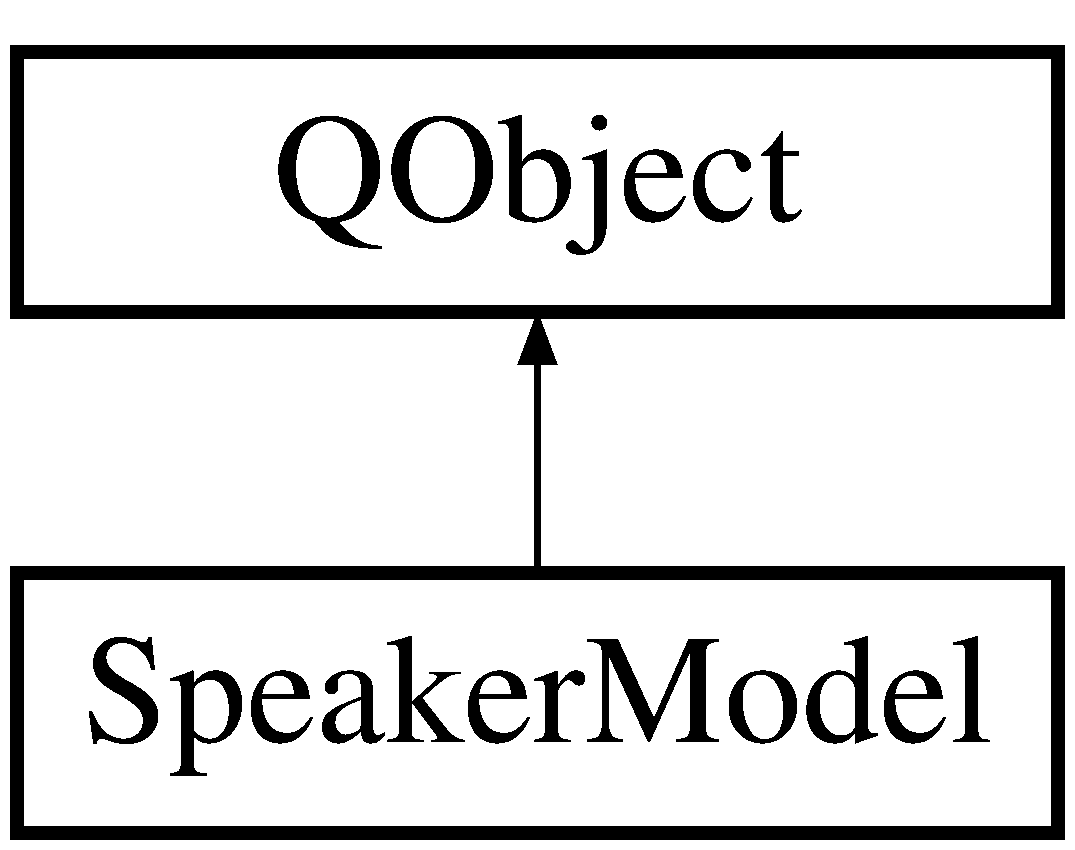
\includegraphics[height=2.000000cm]{classSpeakerModel}
\end{center}
\end{figure}
\subsection*{Public Slots}
\begin{DoxyCompactItemize}
\item 
void \hyperlink{classSpeakerModel_a8c432f96c571375bc177265f1b1cf39f}{reset\-Team} ()
\end{DoxyCompactItemize}
\subsection*{Signals}
\begin{DoxyCompactItemize}
\item 
\hypertarget{classSpeakerModel_abc1e08b179a5be5113c05bb667322d3e}{void {\bfseries name\-Changed} (Q\-String)}\label{classSpeakerModel_abc1e08b179a5be5113c05bb667322d3e}

\item 
\hypertarget{classSpeakerModel_a09c87320b245bf15ff4aa89c02a8e42e}{void {\bfseries is\-Beginner\-Changed} (bool)}\label{classSpeakerModel_a09c87320b245bf15ff4aa89c02a8e42e}

\item 
\hypertarget{classSpeakerModel_a8c98202e34443985f3c978e7c0e12b29}{void {\bfseries opd\-Ffr\-Changed} (bool)}\label{classSpeakerModel_a8c98202e34443985f3c978e7c0e12b29}

\item 
\hypertarget{classSpeakerModel_a3b92430002fe66dc2f27cb2c6a679bc3}{void {\bfseries opd\-Gov\-Changed} (bool)}\label{classSpeakerModel_a3b92430002fe66dc2f27cb2c6a679bc3}

\item 
\hypertarget{classSpeakerModel_aef00e10ddf1b31a6e2cba7ceed0c461c}{void {\bfseries opd\-Op\-Changed} (bool)}\label{classSpeakerModel_aef00e10ddf1b31a6e2cba7ceed0c461c}

\item 
\hypertarget{classSpeakerModel_addf70623030b6a3e7a1722864a4e5e94}{void {\bfseries bps\-Gov\-Changed} (bool)}\label{classSpeakerModel_addf70623030b6a3e7a1722864a4e5e94}

\item 
\hypertarget{classSpeakerModel_ab94f45899981923c871c6c3b25ade0e4}{void {\bfseries bps\-Op\-Changed} (bool)}\label{classSpeakerModel_ab94f45899981923c871c6c3b25ade0e4}

\item 
\hypertarget{classSpeakerModel_ac06b2a9fc7853e9ed8dd604a3d28900c}{void {\bfseries opd\-Jud\-Changed} (bool)}\label{classSpeakerModel_ac06b2a9fc7853e9ed8dd604a3d28900c}

\item 
\hypertarget{classSpeakerModel_a8a6976ca8f4daf01f66cbf88684c14b1}{void {\bfseries bps\-Jud\-Changed} (bool)}\label{classSpeakerModel_a8a6976ca8f4daf01f66cbf88684c14b1}

\item 
\hypertarget{classSpeakerModel_a2c22b4b9bf929b853ff5ccd95c051ffd}{void {\bfseries team\-Changed} (\hyperlink{classSpeakerModel}{Speaker\-Model} $\ast$)}\label{classSpeakerModel_a2c22b4b9bf929b853ff5ccd95c051ffd}

\end{DoxyCompactItemize}
\subsection*{Public Member Functions}
\begin{DoxyCompactItemize}
\item 
\hyperlink{classSpeakerModel_ab277204d896886103f137109b73b961c}{Speaker\-Model} (Q\-Object $\ast$parent=0)
\item 
\hypertarget{classSpeakerModel_a5f62e57052d36ba5f9880882b7a9f4ce}{Q\-String {\bfseries name} ()}\label{classSpeakerModel_a5f62e57052d36ba5f9880882b7a9f4ce}

\item 
\hypertarget{classSpeakerModel_a3045b71845e7a6ecb80f841718456873}{void {\bfseries set\-Name} (Q\-String \hyperlink{classSpeakerModel_a9727f89c2cc146a2d9959d2e692aa444}{name})}\label{classSpeakerModel_a3045b71845e7a6ecb80f841718456873}

\item 
\hypertarget{classSpeakerModel_ac6d6756ae85dc6a2546f18a6e71be095}{bool {\bfseries is\-Beginner} ()}\label{classSpeakerModel_ac6d6756ae85dc6a2546f18a6e71be095}

\item 
\hypertarget{classSpeakerModel_a430365a8afbd64138df99d6908d23334}{void {\bfseries set\-Is\-Beginner} (bool \hyperlink{classSpeakerModel_a47d41be22317dd22fd7aec6240c731cf}{is\-Beginner})}\label{classSpeakerModel_a430365a8afbd64138df99d6908d23334}

\item 
\hypertarget{classSpeakerModel_ac93f7de21450d6bd752890e1e5eeab99}{\hyperlink{classTeam}{Team} $\ast$ {\bfseries team} ()}\label{classSpeakerModel_ac93f7de21450d6bd752890e1e5eeab99}

\item 
\hypertarget{classSpeakerModel_a014f31674707368294e6c3ab067447c3}{void {\bfseries set\-Team} (\hyperlink{classTeam}{Team} $\ast$\hyperlink{classSpeakerModel_a2b6725ebf62712e76c559443426144b1}{team})}\label{classSpeakerModel_a014f31674707368294e6c3ab067447c3}

\item 
\hypertarget{classSpeakerModel_a2bc33b0ddaa652b0e5a000aa67a490d7}{bool {\bfseries opd\-Ffr} ()}\label{classSpeakerModel_a2bc33b0ddaa652b0e5a000aa67a490d7}

\item 
\hypertarget{classSpeakerModel_ae9110f97c46ec0370feb137e7eda015a}{void {\bfseries set\-Opd\-Ffr} (bool \hyperlink{classSpeakerModel_ae7ddef47cf54a9ace7c2399c7a18049d}{opd\-Ffr})}\label{classSpeakerModel_ae9110f97c46ec0370feb137e7eda015a}

\item 
\hypertarget{classSpeakerModel_ab4c1db61647e6870baef318a38199774}{bool {\bfseries opd\-Gov} ()}\label{classSpeakerModel_ab4c1db61647e6870baef318a38199774}

\item 
\hypertarget{classSpeakerModel_a4be095fb20f1713840ec3f27e1b61f30}{void {\bfseries set\-Opd\-Gov} (bool \hyperlink{classSpeakerModel_a7a7dafddf0d9f0bb60e5e138277b50fd}{opd\-Gov})}\label{classSpeakerModel_a4be095fb20f1713840ec3f27e1b61f30}

\item 
\hypertarget{classSpeakerModel_ab21f7d425e31cadc392dfa0bc70ce9c4}{bool {\bfseries opd\-Op} ()}\label{classSpeakerModel_ab21f7d425e31cadc392dfa0bc70ce9c4}

\item 
\hypertarget{classSpeakerModel_a8f5305951717bf934c5bcd17f9a444b2}{void {\bfseries set\-Opd\-Op} (bool \hyperlink{classSpeakerModel_a60ebe1609153ba734e8d5449643cd85e}{opd\-Op})}\label{classSpeakerModel_a8f5305951717bf934c5bcd17f9a444b2}

\item 
\hypertarget{classSpeakerModel_a43e164717e5bf5a373cd5075abdd642e}{bool {\bfseries bps\-Op} ()}\label{classSpeakerModel_a43e164717e5bf5a373cd5075abdd642e}

\item 
\hypertarget{classSpeakerModel_a3f9c08ed9c2ea4b2f262bf8404a56a17}{void {\bfseries set\-Bps\-Op} (bool \hyperlink{classSpeakerModel_a2f2cac7000658283ccf8d06683b64376}{bps\-Op})}\label{classSpeakerModel_a3f9c08ed9c2ea4b2f262bf8404a56a17}

\item 
\hypertarget{classSpeakerModel_a668cf3b29bda7a5681bb82ab4633c111}{bool {\bfseries bps\-Gov} ()}\label{classSpeakerModel_a668cf3b29bda7a5681bb82ab4633c111}

\item 
\hypertarget{classSpeakerModel_ac58a853ced037a112d1ce4a38113739a}{void {\bfseries set\-Bps\-Gov} (bool \hyperlink{classSpeakerModel_aaf2dd2737f827659f7ca2a8a6b8a87f3}{bps\-Gov})}\label{classSpeakerModel_ac58a853ced037a112d1ce4a38113739a}

\item 
\hypertarget{classSpeakerModel_a64af1728737727dabe63fde07ae4506e}{bool {\bfseries opd\-Jud} ()}\label{classSpeakerModel_a64af1728737727dabe63fde07ae4506e}

\item 
\hypertarget{classSpeakerModel_abdc93b6220f71dcb9f3a1802dd55aceb}{void {\bfseries set\-Opd\-Jud} (bool \hyperlink{classSpeakerModel_a427f9e7d98bcbaea06f395eb82271a56}{opd\-Jud})}\label{classSpeakerModel_abdc93b6220f71dcb9f3a1802dd55aceb}

\item 
\hypertarget{classSpeakerModel_a2a81c984fd5b2600088d6d33950972bd}{bool {\bfseries bps\-Jud} ()}\label{classSpeakerModel_a2a81c984fd5b2600088d6d33950972bd}

\item 
\hypertarget{classSpeakerModel_ade12da992153e28d6876b89f20697b7e}{void {\bfseries set\-Bps\-Jud} (bool \hyperlink{classSpeakerModel_a60f2670dcde9e6dbe24661599e6b674c}{bps\-Jud})}\label{classSpeakerModel_ade12da992153e28d6876b89f20697b7e}

\end{DoxyCompactItemize}
\subsection*{Properties}
\begin{DoxyCompactItemize}
\item 
\hypertarget{classSpeakerModel_a9727f89c2cc146a2d9959d2e692aa444}{Q\-String \hyperlink{classSpeakerModel_a9727f89c2cc146a2d9959d2e692aa444}{name}}\label{classSpeakerModel_a9727f89c2cc146a2d9959d2e692aa444}

\begin{DoxyCompactList}\small\item\em The speaker's name. \end{DoxyCompactList}\item 
bool \hyperlink{classSpeakerModel_a47d41be22317dd22fd7aec6240c731cf}{is\-Beginner}
\item 
\hyperlink{classTeam}{Team} \hyperlink{classSpeakerModel_a2b6725ebf62712e76c559443426144b1}{team}
\item 
bool \hyperlink{classSpeakerModel_ae7ddef47cf54a9ace7c2399c7a18049d}{opd\-Ffr}
\item 
bool \hyperlink{classSpeakerModel_a7a7dafddf0d9f0bb60e5e138277b50fd}{opd\-Gov}
\item 
bool \hyperlink{classSpeakerModel_a60ebe1609153ba734e8d5449643cd85e}{opd\-Op}
\item 
bool \hyperlink{classSpeakerModel_aaf2dd2737f827659f7ca2a8a6b8a87f3}{bps\-Gov}
\item 
bool \hyperlink{classSpeakerModel_a2f2cac7000658283ccf8d06683b64376}{bps\-Op}
\item 
bool \hyperlink{classSpeakerModel_a427f9e7d98bcbaea06f395eb82271a56}{opd\-Jud}
\item 
bool \hyperlink{classSpeakerModel_a60f2670dcde9e6dbe24661599e6b674c}{bps\-Jud}
\end{DoxyCompactItemize}


\subsection{Detailed Description}
Represents a speaker in a debate. 

A speaker will be placed on tables according to his properties during the matching process. The speaker can prevent himself from being mapped to certain unwanted positions, marked as a beginner or assigned to a team. 

\subsection{Constructor \& Destructor Documentation}
\hypertarget{classSpeakerModel_ab277204d896886103f137109b73b961c}{\index{Speaker\-Model@{Speaker\-Model}!Speaker\-Model@{Speaker\-Model}}
\index{Speaker\-Model@{Speaker\-Model}!SpeakerModel@{Speaker\-Model}}
\subsubsection[{Speaker\-Model}]{\setlength{\rightskip}{0pt plus 5cm}Speaker\-Model\-::\-Speaker\-Model (
\begin{DoxyParamCaption}
\item[{Q\-Object $\ast$}]{parent = {\ttfamily 0}}
\end{DoxyParamCaption}
)}}\label{classSpeakerModel_ab277204d896886103f137109b73b961c}
Creates a new speaker without any role restrictions. The speaker is set as no beginner and has no team. 

\subsection{Member Function Documentation}
\hypertarget{classSpeakerModel_a8c432f96c571375bc177265f1b1cf39f}{\index{Speaker\-Model@{Speaker\-Model}!reset\-Team@{reset\-Team}}
\index{reset\-Team@{reset\-Team}!SpeakerModel@{Speaker\-Model}}
\subsubsection[{reset\-Team}]{\setlength{\rightskip}{0pt plus 5cm}void Speaker\-Model\-::reset\-Team (
\begin{DoxyParamCaption}
{}
\end{DoxyParamCaption}
)\hspace{0.3cm}{\ttfamily [inline]}, {\ttfamily [slot]}}}\label{classSpeakerModel_a8c432f96c571375bc177265f1b1cf39f}
Same as 
\begin{DoxyCode}
setTeam(NULL) 
\end{DoxyCode}
 \begin{DoxySeeAlso}{See Also}
set\-Team 
\end{DoxySeeAlso}


\subsection{Property Documentation}
\hypertarget{classSpeakerModel_aaf2dd2737f827659f7ca2a8a6b8a87f3}{\index{Speaker\-Model@{Speaker\-Model}!bps\-Gov@{bps\-Gov}}
\index{bps\-Gov@{bps\-Gov}!SpeakerModel@{Speaker\-Model}}
\subsubsection[{bps\-Gov}]{\setlength{\rightskip}{0pt plus 5cm}bool Speaker\-Model\-::bps\-Gov\hspace{0.3cm}{\ttfamily [read]}, {\ttfamily [write]}}}\label{classSpeakerModel_aaf2dd2737f827659f7ca2a8a6b8a87f3}
Holds if the speaker can be mapped to the government side in an B\-P\-S-\/debate. \begin{DoxySeeAlso}{See Also}
\hyperlink{classBPSDebate}{B\-P\-S\-Debate} 
\end{DoxySeeAlso}
\hypertarget{classSpeakerModel_a60f2670dcde9e6dbe24661599e6b674c}{\index{Speaker\-Model@{Speaker\-Model}!bps\-Jud@{bps\-Jud}}
\index{bps\-Jud@{bps\-Jud}!SpeakerModel@{Speaker\-Model}}
\subsubsection[{bps\-Jud}]{\setlength{\rightskip}{0pt plus 5cm}bool Speaker\-Model\-::bps\-Jud\hspace{0.3cm}{\ttfamily [read]}, {\ttfamily [write]}}}\label{classSpeakerModel_a60f2670dcde9e6dbe24661599e6b674c}
Holds if the speaker can be set to judicate an B\-P\-S-\/debate. \begin{DoxySeeAlso}{See Also}
\hyperlink{classDebate}{Debate} 
\end{DoxySeeAlso}
\hypertarget{classSpeakerModel_a2f2cac7000658283ccf8d06683b64376}{\index{Speaker\-Model@{Speaker\-Model}!bps\-Op@{bps\-Op}}
\index{bps\-Op@{bps\-Op}!SpeakerModel@{Speaker\-Model}}
\subsubsection[{bps\-Op}]{\setlength{\rightskip}{0pt plus 5cm}bool Speaker\-Model\-::bps\-Op\hspace{0.3cm}{\ttfamily [read]}, {\ttfamily [write]}}}\label{classSpeakerModel_a2f2cac7000658283ccf8d06683b64376}
Holds if the speaker can be mapped to the oppositoin side in an B\-P\-S-\/debate. \begin{DoxySeeAlso}{See Also}
\hyperlink{classBPSDebate}{B\-P\-S\-Debate} 
\end{DoxySeeAlso}
\hypertarget{classSpeakerModel_a47d41be22317dd22fd7aec6240c731cf}{\index{Speaker\-Model@{Speaker\-Model}!is\-Beginner@{is\-Beginner}}
\index{is\-Beginner@{is\-Beginner}!SpeakerModel@{Speaker\-Model}}
\subsubsection[{is\-Beginner}]{\setlength{\rightskip}{0pt plus 5cm}bool Speaker\-Model\-::is\-Beginner\hspace{0.3cm}{\ttfamily [read]}, {\ttfamily [write]}}}\label{classSpeakerModel_a47d41be22317dd22fd7aec6240c731cf}
Holds if the speaker is a beginner. Beginners won't be in the same team. \hypertarget{classSpeakerModel_ae7ddef47cf54a9ace7c2399c7a18049d}{\index{Speaker\-Model@{Speaker\-Model}!opd\-Ffr@{opd\-Ffr}}
\index{opd\-Ffr@{opd\-Ffr}!SpeakerModel@{Speaker\-Model}}
\subsubsection[{opd\-Ffr}]{\setlength{\rightskip}{0pt plus 5cm}bool Speaker\-Model\-::opd\-Ffr\hspace{0.3cm}{\ttfamily [read]}, {\ttfamily [write]}}}\label{classSpeakerModel_ae7ddef47cf54a9ace7c2399c7a18049d}
Holds if the the speaker can be mapped to the F\-F\-R-\/role of an O\-P-\/debate. \begin{DoxySeeAlso}{See Also}
O\-P\-D\-Debate 
\end{DoxySeeAlso}
\hypertarget{classSpeakerModel_a7a7dafddf0d9f0bb60e5e138277b50fd}{\index{Speaker\-Model@{Speaker\-Model}!opd\-Gov@{opd\-Gov}}
\index{opd\-Gov@{opd\-Gov}!SpeakerModel@{Speaker\-Model}}
\subsubsection[{opd\-Gov}]{\setlength{\rightskip}{0pt plus 5cm}bool Speaker\-Model\-::opd\-Gov\hspace{0.3cm}{\ttfamily [read]}, {\ttfamily [write]}}}\label{classSpeakerModel_a7a7dafddf0d9f0bb60e5e138277b50fd}
Holds if the speaker can be mapped to the government side in an O\-P-\/debate. \begin{DoxySeeAlso}{See Also}
O\-P\-D\-Debate 
\end{DoxySeeAlso}
\hypertarget{classSpeakerModel_a427f9e7d98bcbaea06f395eb82271a56}{\index{Speaker\-Model@{Speaker\-Model}!opd\-Jud@{opd\-Jud}}
\index{opd\-Jud@{opd\-Jud}!SpeakerModel@{Speaker\-Model}}
\subsubsection[{opd\-Jud}]{\setlength{\rightskip}{0pt plus 5cm}bool Speaker\-Model\-::opd\-Jud\hspace{0.3cm}{\ttfamily [read]}, {\ttfamily [write]}}}\label{classSpeakerModel_a427f9e7d98bcbaea06f395eb82271a56}
Holds if the speaker can be set to judicate an O\-P-\/debate. \begin{DoxySeeAlso}{See Also}
\hyperlink{classDebate}{Debate} 
\end{DoxySeeAlso}
\hypertarget{classSpeakerModel_a60ebe1609153ba734e8d5449643cd85e}{\index{Speaker\-Model@{Speaker\-Model}!opd\-Op@{opd\-Op}}
\index{opd\-Op@{opd\-Op}!SpeakerModel@{Speaker\-Model}}
\subsubsection[{opd\-Op}]{\setlength{\rightskip}{0pt plus 5cm}bool Speaker\-Model\-::opd\-Op\hspace{0.3cm}{\ttfamily [read]}, {\ttfamily [write]}}}\label{classSpeakerModel_a60ebe1609153ba734e8d5449643cd85e}
Holds if the speaker can be mapped to the opposition side in an O\-P-\/debate. \begin{DoxySeeAlso}{See Also}
O\-P\-D\-Debate 
\end{DoxySeeAlso}
\hypertarget{classSpeakerModel_a2b6725ebf62712e76c559443426144b1}{\index{Speaker\-Model@{Speaker\-Model}!team@{team}}
\index{team@{team}!SpeakerModel@{Speaker\-Model}}
\subsubsection[{team}]{\setlength{\rightskip}{0pt plus 5cm}{\bf Team} Speaker\-Model\-::team\hspace{0.3cm}{\ttfamily [read]}, {\ttfamily [write]}}}\label{classSpeakerModel_a2b6725ebf62712e76c559443426144b1}
The speaker's team or {\ttfamily N\-U\-L\-L} if he is not member of a team. Setting this property will add the speaker to the team's speaker list. Setting a value of {\ttfamily N\-U\-L\-L} will delete the speaker from the team's speaker list. Destroying the team will set this property to {\ttfamily N\-U\-L\-L} 

The documentation for this class was generated from the following files\-:\begin{DoxyCompactItemize}
\item 
/home/stoef/qt/projects/ddt/ddt/src/speakermodel.\-h\item 
/home/stoef/qt/projects/ddt/ddt/src/speakermodel.\-cpp\end{DoxyCompactItemize}

\hypertarget{classSpeakerPage}{\section{Speaker\-Page Class Reference}
\label{classSpeakerPage}\index{Speaker\-Page@{Speaker\-Page}}
}


A component that allows the selection and editing of on ore more speakers.  


Inheritance diagram for Speaker\-Page\-:\begin{figure}[H]
\begin{center}
\leavevmode
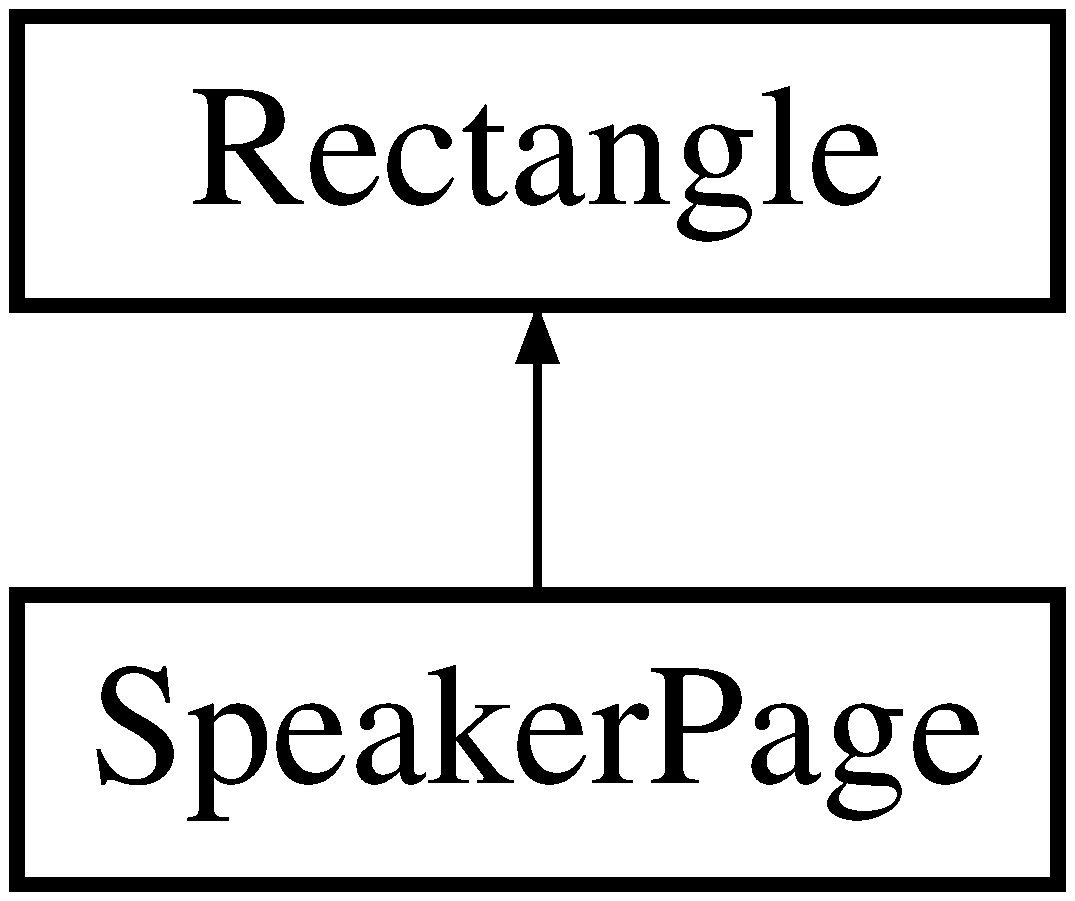
\includegraphics[height=2.000000cm]{classSpeakerPage}
\end{center}
\end{figure}
\subsection*{Properties}
\begin{DoxyCompactItemize}
\item 
\hypertarget{classSpeakerPage_a3e35e3c23d511c7a048494deb3de57e8}{Component \hyperlink{classSpeakerPage_a3e35e3c23d511c7a048494deb3de57e8}{tool\-Bar\-Component}}\label{classSpeakerPage_a3e35e3c23d511c7a048494deb3de57e8}

\begin{DoxyCompactList}\small\item\em The page's toolbar additions. \end{DoxyCompactList}\item 
\hypertarget{classSpeakerPage_aca9be87a6fcb6622833e87861f3a92a7}{Q\-List\-Q\-M\-L\-Wrapper \hyperlink{classSpeakerPage_aca9be87a6fcb6622833e87861f3a92a7}{selection\-Model}}\label{classSpeakerPage_aca9be87a6fcb6622833e87861f3a92a7}

\begin{DoxyCompactList}\small\item\em The application's selection model. This is a list containing {\ttfamily \hyperlink{classSpeakerModel}{Speaker\-Model}} objects. \end{DoxyCompactList}\item 
\hypertarget{classSpeakerPage_a334a8bee32e6e8f32bbbd6c0836565e1}{\hyperlink{classMainModel}{Main\-Model} \hyperlink{classSpeakerPage_a334a8bee32e6e8f32bbbd6c0836565e1}{main\-Model}}\label{classSpeakerPage_a334a8bee32e6e8f32bbbd6c0836565e1}

\begin{DoxyCompactList}\small\item\em The application's {\ttfamily \hyperlink{classMainModel}{Main\-Model}}. \end{DoxyCompactList}\item 
\hypertarget{classSpeakerPage_ae1b16972611aaba445364e17ca414264}{Action \hyperlink{classSpeakerPage_ae1b16972611aaba445364e17ca414264}{add\-Speaker\-Action}}\label{classSpeakerPage_ae1b16972611aaba445364e17ca414264}

\begin{DoxyCompactList}\small\item\em An action that adds a speaker. \end{DoxyCompactList}\end{DoxyCompactItemize}


\subsection{Detailed Description}
A component that allows the selection and editing of on ore more speakers. 

The component consists of two parts\-: A {\ttfamily \hyperlink{classSpeakerList}{Speaker\-List}} , allowing to select various speakers, and an {\ttfamily \hyperlink{classAllowedRolesEditor}{Allowed\-Roles\-Editor}} which allows the editing of the selected speakers properties. Additionally, a {\ttfamily \hyperlink{classTeamEditor}{Team\-Editor}} is used which enables the editing of teams. 

The documentation for this class was generated from the following file\-:\begin{DoxyCompactItemize}
\item 
/home/stoef/qt/projects/ddt/ddt/qml/ddt/Speaker\-Page.\-qml\end{DoxyCompactItemize}

\hypertarget{classTable}{\section{Table Class Reference}
\label{classTable}\index{Table@{Table}}
}


Displays a debate's table and all enabled team seats.  


Inheritance diagram for Table\-:\begin{figure}[H]
\begin{center}
\leavevmode
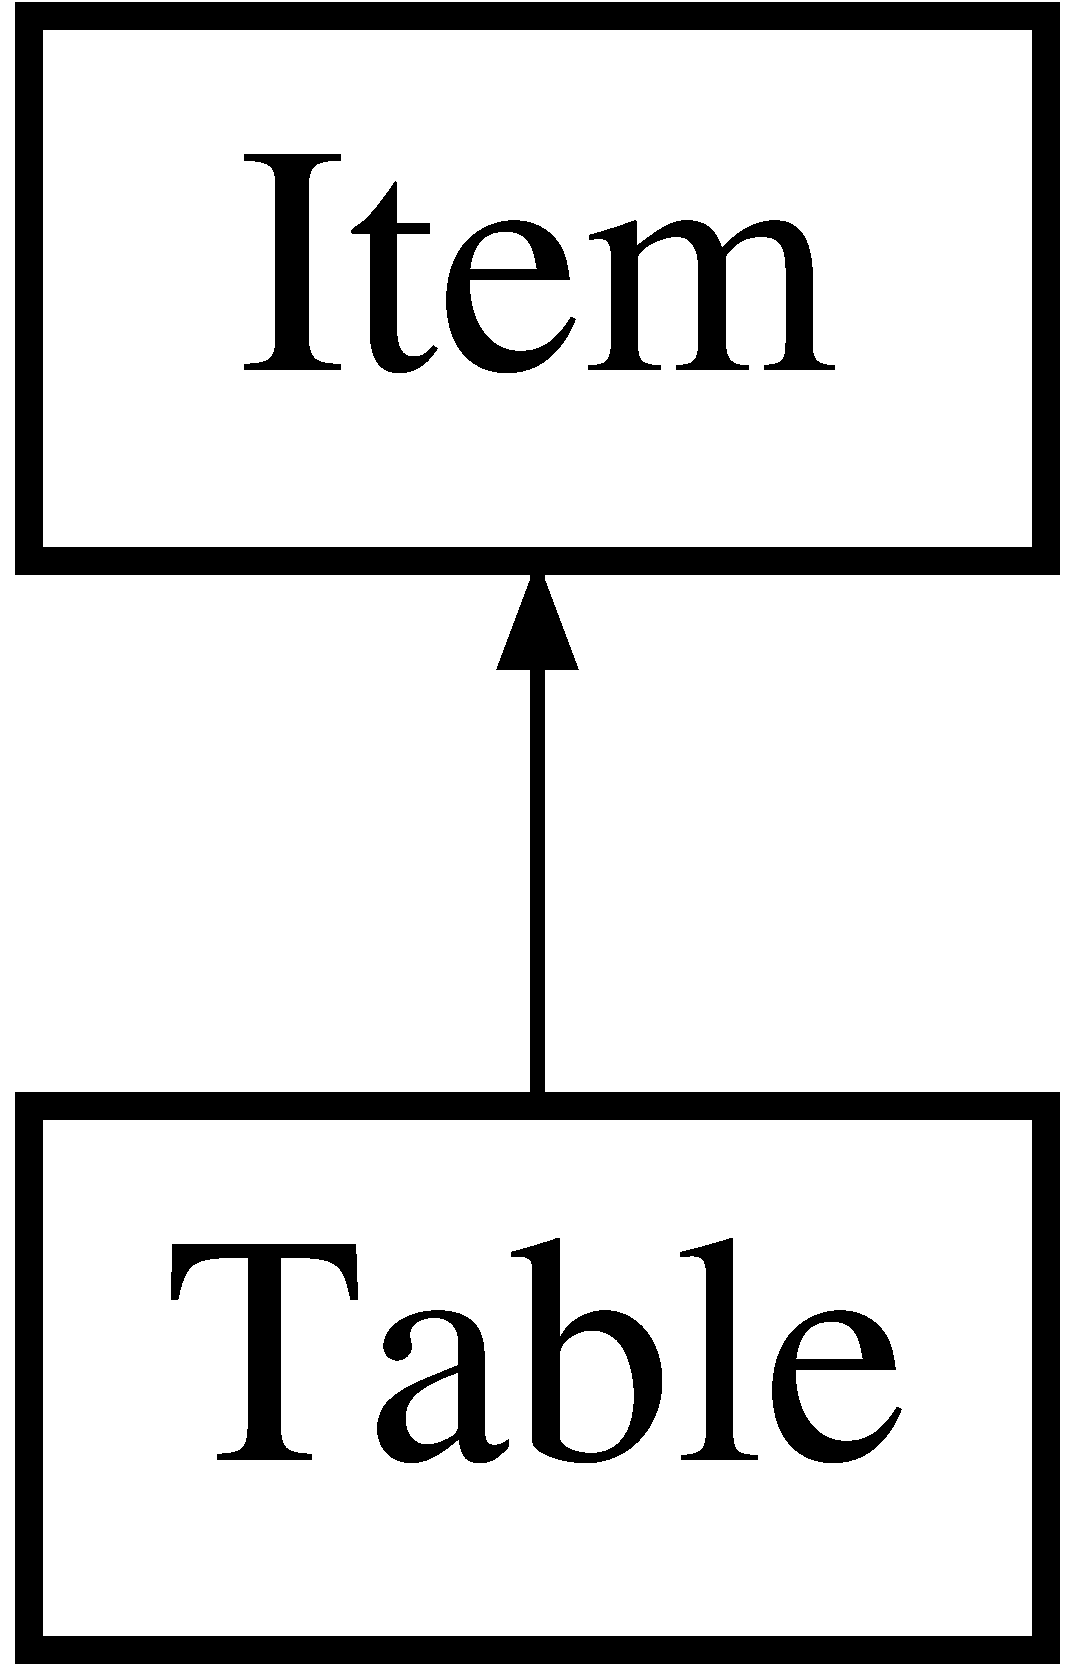
\includegraphics[height=2.000000cm]{classTable}
\end{center}
\end{figure}
\subsection*{Signals}
\begin{DoxyCompactItemize}
\item 
void \hyperlink{classTable_a6d82e2f7c1b669222fd22ad42f5b92c8}{increment} ()
\item 
void \hyperlink{classTable_ab6d6f8837a696567a11b509357529954}{decrement} ()
\end{DoxyCompactItemize}
\subsection*{Properties}
\begin{DoxyCompactItemize}
\item 
\hyperlink{classTableNames}{Table\-Names} \hyperlink{classTable_acdcaaceb37a19b80750e2b5e1c75cc63}{names}
\item 
\hypertarget{classTable_ab401fbfc271b2efc72679916bd055bc6}{int \hyperlink{classTable_ab401fbfc271b2efc72679916bd055bc6}{seat\-Count}}\label{classTable_ab401fbfc271b2efc72679916bd055bc6}

\begin{DoxyCompactList}\small\item\em Holds how many seats are currently being displayed. \end{DoxyCompactList}\item 
\hypertarget{classTable_a3c3a525011e324c966b3753eed579d78}{bool \hyperlink{classTable_a3c3a525011e324c966b3753eed579d78}{editable}}\label{classTable_a3c3a525011e324c966b3753eed579d78}

\begin{DoxyCompactList}\small\item\em Specifies if the seat count can be edited. \end{DoxyCompactList}\item 
alias \hyperlink{classTable_a99ba041de21998ee2f001613334e2b73}{table\-Text}
\item 
int \hyperlink{classTable_adb0d1c7f4d3581f19f370429d6b88241}{preferred\-Seat\-Count}
\item 
\hypertarget{classTable_ab0953083ef1c8e632e10f0828c971b24}{int \hyperlink{classTable_ab0953083ef1c8e632e10f0828c971b24}{max\-Seat\-Count}}\label{classTable_ab0953083ef1c8e632e10f0828c971b24}

\begin{DoxyCompactList}\small\item\em Specifies how many seats the table can hold at most. \end{DoxyCompactList}\item 
\hypertarget{classTable_a4c7d9044fbec7afa25a9f1be38a44a1f}{int \hyperlink{classTable_a4c7d9044fbec7afa25a9f1be38a44a1f}{\-\_\-\-\_\-seat\-Diameter}}\label{classTable_a4c7d9044fbec7afa25a9f1be38a44a1f}

\begin{DoxyCompactList}\small\item\em Internal. \end{DoxyCompactList}\item 
alias \hyperlink{classTable_a0fd0e5c3c8de91f59a26c3e6ec0aa149}{table\-Rotation}
\item 
alias \hyperlink{classTable_acc1414efc33cc8a93d1c36ee2b81ef88}{rotation\-Origin}
\end{DoxyCompactItemize}


\subsection{Detailed Description}
Displays a debate's table and all enabled team seats. 

A table in a debate specifies how many seats are reserved for a specific team (e.\-g. how many judicators or speakers of the government take part in a debate). Furthermore, the number of seats can be edited. The individual seats may be labeled with an arbitrary string, usually the speaker's name. 

\subsection{Member Function Documentation}
\hypertarget{classTable_ab6d6f8837a696567a11b509357529954}{\index{Table@{Table}!decrement@{decrement}}
\index{decrement@{decrement}!Table@{Table}}
\subsubsection[{decrement}]{\setlength{\rightskip}{0pt plus 5cm}void Table\-::decrement (
\begin{DoxyParamCaption}
{}
\end{DoxyParamCaption}
)\hspace{0.3cm}{\ttfamily [signal]}}}\label{classTable_ab6d6f8837a696567a11b509357529954}
Called whenever the user indicates that he or she wants to remove a seat from the table. \hypertarget{classTable_a6d82e2f7c1b669222fd22ad42f5b92c8}{\index{Table@{Table}!increment@{increment}}
\index{increment@{increment}!Table@{Table}}
\subsubsection[{increment}]{\setlength{\rightskip}{0pt plus 5cm}void Table\-::increment (
\begin{DoxyParamCaption}
{}
\end{DoxyParamCaption}
)\hspace{0.3cm}{\ttfamily [signal]}}}\label{classTable_a6d82e2f7c1b669222fd22ad42f5b92c8}
Called whenever the user indicates that he or she wants to add a new seat to the table. 

\subsection{Property Documentation}
\hypertarget{classTable_acdcaaceb37a19b80750e2b5e1c75cc63}{\index{Table@{Table}!names@{names}}
\index{names@{names}!Table@{Table}}
\subsubsection[{names}]{\setlength{\rightskip}{0pt plus 5cm}{\bf Table\-Names} Table\-::names}}\label{classTable_acdcaaceb37a19b80750e2b5e1c75cc63}
This property is either {\ttfamily null} or maps an arbitrary label to each seat. This label is displayed at each seat. \hypertarget{classTable_adb0d1c7f4d3581f19f370429d6b88241}{\index{Table@{Table}!preferred\-Seat\-Count@{preferred\-Seat\-Count}}
\index{preferred\-Seat\-Count@{preferred\-Seat\-Count}!Table@{Table}}
\subsubsection[{preferred\-Seat\-Count}]{\setlength{\rightskip}{0pt plus 5cm}int Table\-::preferred\-Seat\-Count}}\label{classTable_adb0d1c7f4d3581f19f370429d6b88241}
Holds how many seats should be set in a perfectly set debate. This will influence the displayed length of the table. \hypertarget{classTable_acc1414efc33cc8a93d1c36ee2b81ef88}{\index{Table@{Table}!rotation\-Origin@{rotation\-Origin}}
\index{rotation\-Origin@{rotation\-Origin}!Table@{Table}}
\subsubsection[{rotation\-Origin}]{\setlength{\rightskip}{0pt plus 5cm}alias Table\-::rotation\-Origin}}\label{classTable_acc1414efc33cc8a93d1c36ee2b81ef88}
The table's rotation origin. Use this instead of {\ttfamily Item.\-transform\-Origin} to achieve a better useable and readable rotation. \hypertarget{classTable_a0fd0e5c3c8de91f59a26c3e6ec0aa149}{\index{Table@{Table}!table\-Rotation@{table\-Rotation}}
\index{table\-Rotation@{table\-Rotation}!Table@{Table}}
\subsubsection[{table\-Rotation}]{\setlength{\rightskip}{0pt plus 5cm}alias Table\-::table\-Rotation}}\label{classTable_a0fd0e5c3c8de91f59a26c3e6ec0aa149}
The table's rotation. Use this instead of {\ttfamily Item.\-rotation} to achieve a better useable and readable rotation. \hypertarget{classTable_a99ba041de21998ee2f001613334e2b73}{\index{Table@{Table}!table\-Text@{table\-Text}}
\index{table\-Text@{table\-Text}!Table@{Table}}
\subsubsection[{table\-Text}]{\setlength{\rightskip}{0pt plus 5cm}alias Table\-::table\-Text}}\label{classTable_a99ba041de21998ee2f001613334e2b73}
Holds a text that is displayed within the table. This can be used to display which team is seated at this table. 

The documentation for this class was generated from the following file\-:\begin{DoxyCompactItemize}
\item 
/home/stoef/qt/projects/ddt/ddt/qml/ddt/Table.\-qml\end{DoxyCompactItemize}

\hypertarget{classTableNames}{\section{Table\-Names Class Reference}
\label{classTableNames}\index{Table\-Names@{Table\-Names}}
}


Stores speakers mapped to a table in a debate.  




{\ttfamily \#include $<$tablenames.\-h$>$}

Inheritance diagram for Table\-Names\-:\begin{figure}[H]
\begin{center}
\leavevmode
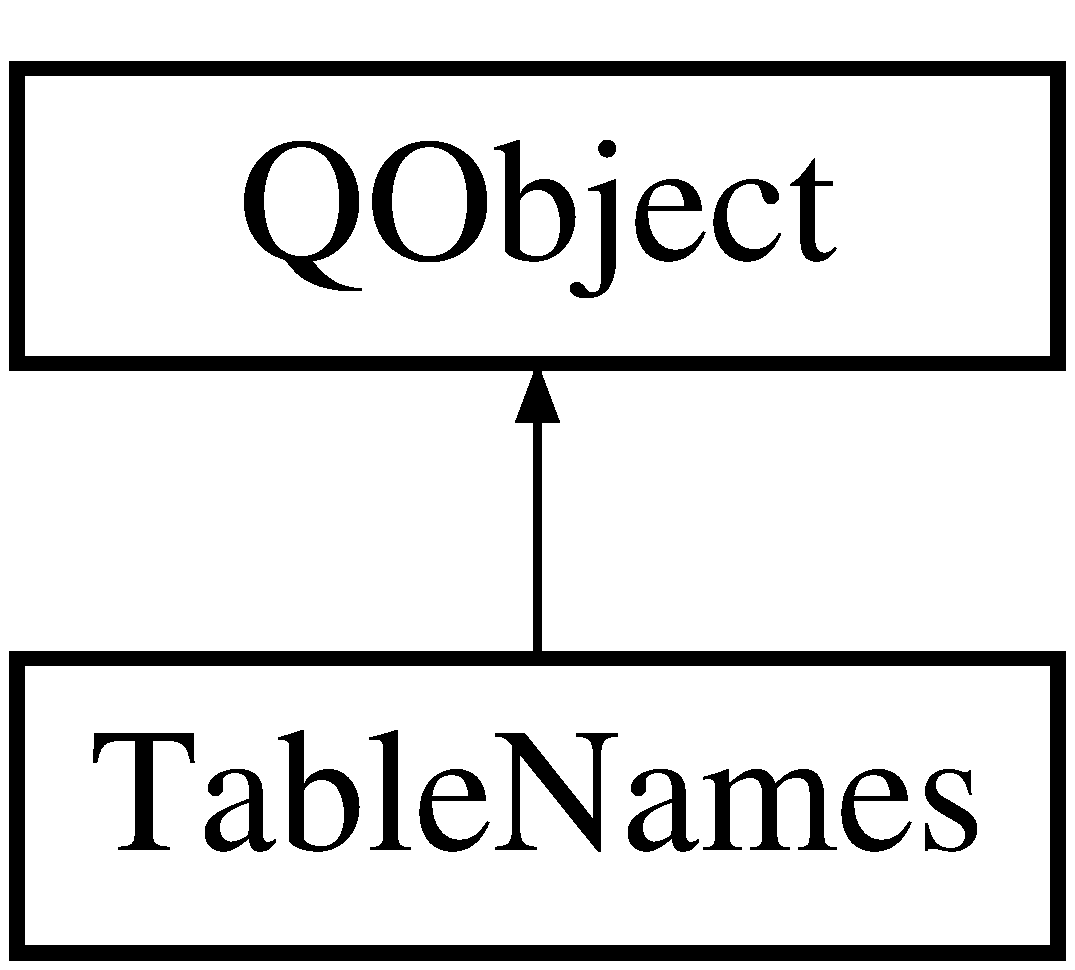
\includegraphics[height=2.000000cm]{classTableNames}
\end{center}
\end{figure}
\subsection*{Public Member Functions}
\begin{DoxyCompactItemize}
\item 
\hypertarget{classTableNames_a8c8d9e635a104088b62c26734084d760}{\hyperlink{classTableNames_a8c8d9e635a104088b62c26734084d760}{Table\-Names} (Q\-Object $\ast$parent=0)}\label{classTableNames_a8c8d9e635a104088b62c26734084d760}

\begin{DoxyCompactList}\small\item\em Creates a new {\ttfamily \hyperlink{classTableNames}{Table\-Names}} object with a given parent. \end{DoxyCompactList}\item 
\hypertarget{classTableNames_a996257dd574af5f4381f1295d2b8eb15}{Q\-\_\-\-I\-N\-V\-O\-K\-A\-B\-L\-E \hyperlink{classSpeakerModel}{Speaker\-Model} $\ast$ \hyperlink{classTableNames_a996257dd574af5f4381f1295d2b8eb15}{get\-Speaker} (int index)}\label{classTableNames_a996257dd574af5f4381f1295d2b8eb15}

\begin{DoxyCompactList}\small\item\em Gets the speaker sitting at {\ttfamily index}. \end{DoxyCompactList}\item 
\hypertarget{classTableNames_a66a67aef763ec356e52382061bd1f1a1}{void \hyperlink{classTableNames_a66a67aef763ec356e52382061bd1f1a1}{add\-Mapping} (int index, \hyperlink{classSpeakerModel}{Speaker\-Model} $\ast$speaker)}\label{classTableNames_a66a67aef763ec356e52382061bd1f1a1}

\begin{DoxyCompactList}\small\item\em Defines the speaker sitting at {\ttfamily index}. \end{DoxyCompactList}\end{DoxyCompactItemize}


\subsection{Detailed Description}
Stores speakers mapped to a table in a debate. 

The documentation for this class was generated from the following files\-:\begin{DoxyCompactItemize}
\item 
/home/stoef/qt/projects/ddt/ddt/src/tablenames.\-h\item 
/home/stoef/qt/projects/ddt/ddt/src/tablenames.\-cpp\end{DoxyCompactItemize}

\hypertarget{classTeam}{\section{Team Class Reference}
\label{classTeam}\index{Team@{Team}}
}


Represents a team in a debate.  




{\ttfamily \#include $<$team.\-h$>$}

Inheritance diagram for Team\-:\begin{figure}[H]
\begin{center}
\leavevmode
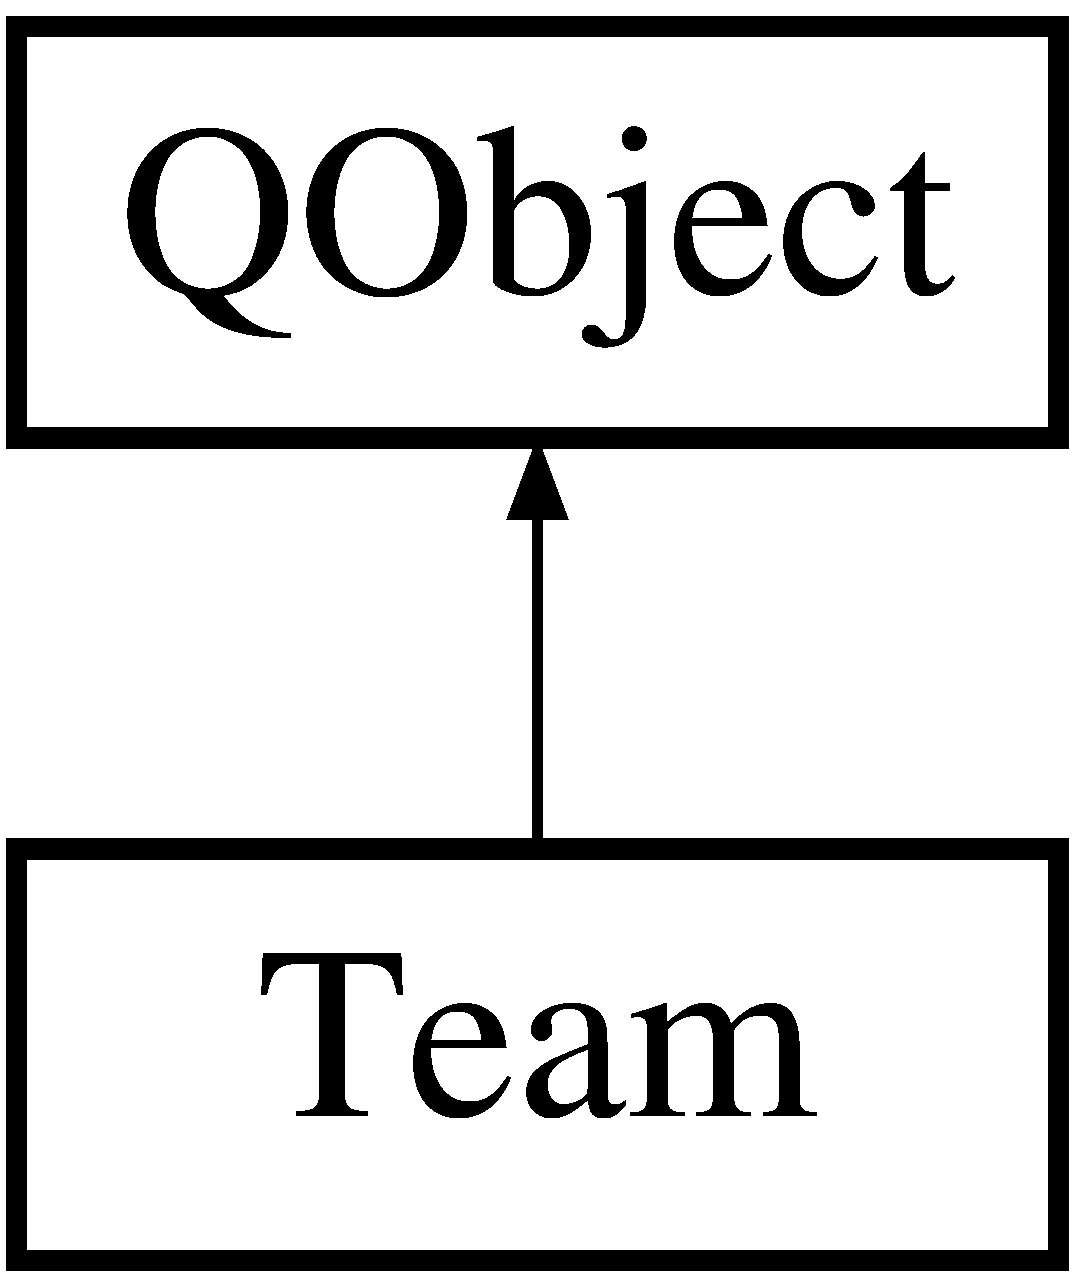
\includegraphics[height=2.000000cm]{classTeam}
\end{center}
\end{figure}
\subsection*{Signals}
\begin{DoxyCompactItemize}
\item 
\hypertarget{classTeam_a29e138b413efaefa54d7e0c36a397ace}{void \hyperlink{classTeam_a29e138b413efaefa54d7e0c36a397ace}{speakers\-Changed} ()}\label{classTeam_a29e138b413efaefa54d7e0c36a397ace}

\begin{DoxyCompactList}\small\item\em Emitted when a speaker was added or removed. \end{DoxyCompactList}\item 
\hypertarget{classTeam_aefee2bc5f2ca783dfe4ab63a4926128d}{void {\bfseries team\-Name\-Changed} ()}\label{classTeam_aefee2bc5f2ca783dfe4ab63a4926128d}

\end{DoxyCompactItemize}
\subsection*{Public Member Functions}
\begin{DoxyCompactItemize}
\item 
\hypertarget{classTeam_afac346a2380d0c8d44e036f3546724fd}{\hyperlink{classTeam_afac346a2380d0c8d44e036f3546724fd}{Team} (Q\-Object $\ast$parent=0)}\label{classTeam_afac346a2380d0c8d44e036f3546724fd}

\begin{DoxyCompactList}\small\item\em Creates a new team with no speakers. \end{DoxyCompactList}\item 
\hypertarget{classTeam_a5580d0af7691668b06f8b12e36f256ae}{Q\-String {\bfseries team\-Name} ()}\label{classTeam_a5580d0af7691668b06f8b12e36f256ae}

\item 
\hypertarget{classTeam_a1ea161f9bcc465d45a8ca2603590739e}{void {\bfseries set\-Team\-Name} (Q\-String team\-Name)}\label{classTeam_a1ea161f9bcc465d45a8ca2603590739e}

\item 
\hypertarget{classTeam_a119572f6c2b161793e6e0142eaaa6662}{void \hyperlink{classTeam_a119572f6c2b161793e6e0142eaaa6662}{add\-Speaker} (\hyperlink{classSpeakerModel}{Speaker\-Model} $\ast$speaker)}\label{classTeam_a119572f6c2b161793e6e0142eaaa6662}

\begin{DoxyCompactList}\small\item\em Adds a speaker to this team. \end{DoxyCompactList}\item 
\hypertarget{classTeam_a4498bf1abc95c7ac84317e3c0ab1f5ac}{bool \hyperlink{classTeam_a4498bf1abc95c7ac84317e3c0ab1f5ac}{contains\-Speaker} (\hyperlink{classSpeakerModel}{Speaker\-Model} $\ast$speaker)}\label{classTeam_a4498bf1abc95c7ac84317e3c0ab1f5ac}

\begin{DoxyCompactList}\small\item\em Returns {\ttfamily true} if a speaker is contained in a specific team. \end{DoxyCompactList}\item 
\hypertarget{classTeam_a59ac03f8a3f9448b20bfd16c2ad64f04}{const Q\-List$<$ \hyperlink{classSpeakerModel}{Speaker\-Model} $\ast$ $>$ $\ast$ \hyperlink{classTeam_a59ac03f8a3f9448b20bfd16c2ad64f04}{get\-Speakers} ()}\label{classTeam_a59ac03f8a3f9448b20bfd16c2ad64f04}

\begin{DoxyCompactList}\small\item\em Returns all speakers of this team. \end{DoxyCompactList}\item 
\hypertarget{classTeam_aa64df580e27d1e27b3ced935fa9659f9}{Q\-\_\-\-I\-N\-V\-O\-K\-A\-B\-L\-E \hyperlink{classSpeakerModel}{Speaker\-Model} $\ast$ \hyperlink{classTeam_aa64df580e27d1e27b3ced935fa9659f9}{get\-Speaker} (int index)}\label{classTeam_aa64df580e27d1e27b3ced935fa9659f9}

\begin{DoxyCompactList}\small\item\em Returns the speaker with a given index. \end{DoxyCompactList}\item 
\hypertarget{classTeam_a88ff24cc77f3c1695dbbf26c6c51012c}{Q\-\_\-\-I\-N\-V\-O\-K\-A\-B\-L\-E int \hyperlink{classTeam_a88ff24cc77f3c1695dbbf26c6c51012c}{speaker\-Count} ()}\label{classTeam_a88ff24cc77f3c1695dbbf26c6c51012c}

\begin{DoxyCompactList}\small\item\em Returns the number of speakers in this team. \end{DoxyCompactList}\item 
\hypertarget{classTeam_abdd95ad8dae4c5fa9b2bfdf199c1fa2f}{Q\-\_\-\-I\-N\-V\-O\-K\-A\-B\-L\-E void \hyperlink{classTeam_abdd95ad8dae4c5fa9b2bfdf199c1fa2f}{remove\-Speaker} (int index)}\label{classTeam_abdd95ad8dae4c5fa9b2bfdf199c1fa2f}

\begin{DoxyCompactList}\small\item\em Removes the speaker with a given index. \end{DoxyCompactList}\end{DoxyCompactItemize}
\subsection*{Properties}
\begin{DoxyCompactItemize}
\item 
\hypertarget{classTeam_a9c0ae7e7f136221e0557aeec458b3a66}{Q\-String {\bfseries team\-Name}}\label{classTeam_a9c0ae7e7f136221e0557aeec458b3a66}

\end{DoxyCompactItemize}


\subsection{Detailed Description}
Represents a team in a debate. 

A team consists of several speakers which will be matched to the same role. Deleting a speaker will automatically remove him from the team. 

The documentation for this class was generated from the following files\-:\begin{DoxyCompactItemize}
\item 
/home/stoef/qt/projects/ddt/ddt/src/team.\-h\item 
/home/stoef/qt/projects/ddt/ddt/src/team.\-cpp\end{DoxyCompactItemize}

\hypertarget{classTeamEditor}{\section{Team\-Editor Class Reference}
\label{classTeamEditor}\index{Team\-Editor@{Team\-Editor}}
}


An editor allowing the editing of teams.  


Inheritance diagram for Team\-Editor\-:\begin{figure}[H]
\begin{center}
\leavevmode
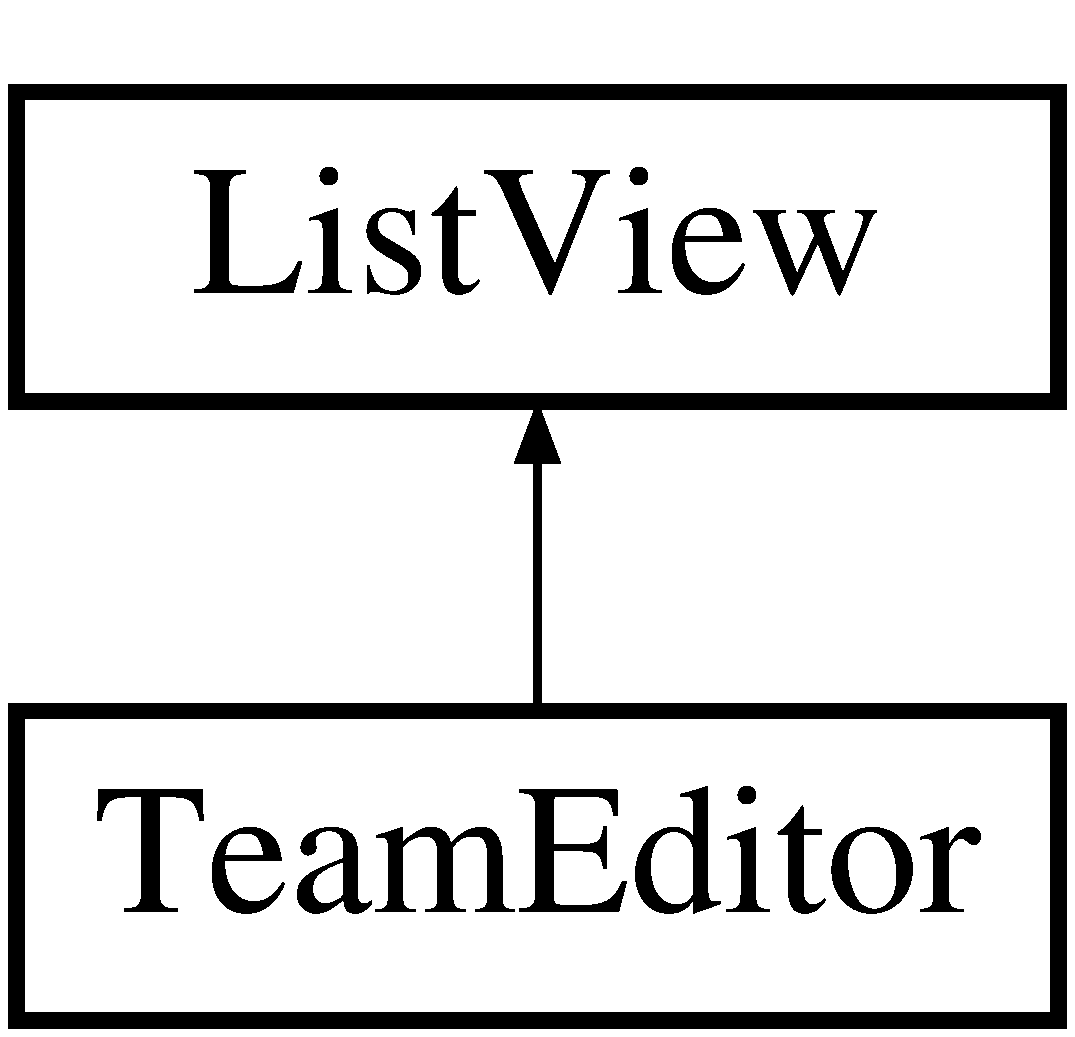
\includegraphics[height=2.000000cm]{classTeamEditor}
\end{center}
\end{figure}
\subsection*{Properties}
\begin{DoxyCompactItemize}
\item 
\hypertarget{classTeamEditor_a215894d4698769bad1cfed7c4d05edfd}{Q\-List\-Q\-M\-L\-Wrapper \hyperlink{classTeamEditor_a215894d4698769bad1cfed7c4d05edfd}{teams}}\label{classTeamEditor_a215894d4698769bad1cfed7c4d05edfd}

\begin{DoxyCompactList}\small\item\em A List containing all current \hyperlink{classTeam}{Team} objects. \end{DoxyCompactList}\item 
\hypertarget{classTeamEditor_a82d28b574654b5d7e691c80cd11384fe}{Q\-List\-Q\-M\-L\-Wrapper \hyperlink{classTeamEditor_a82d28b574654b5d7e691c80cd11384fe}{selection\-Model}}\label{classTeamEditor_a82d28b574654b5d7e691c80cd11384fe}

\begin{DoxyCompactList}\small\item\em A selection model holding the currently selected \hyperlink{classSpeakerModel}{Speaker\-Model} objects. \end{DoxyCompactList}\end{DoxyCompactItemize}


\subsection{Detailed Description}
An editor allowing the editing of teams. 

The editor allows for operations\-:
\begin{DoxyItemize}
\item Add all selected speakers (according to a selection model) to some team
\item Move a speaker into another team (by drag \& drop)
\item remove a team (the speakers won't be removed)
\item Edit a team's name 
\end{DoxyItemize}

The documentation for this class was generated from the following file\-:\begin{DoxyCompactItemize}
\item 
/home/stoef/qt/projects/ddt/ddt/qml/ddt/Team\-Editor.\-qml\end{DoxyCompactItemize}

\hypertarget{classTriCell}{\section{Tri\-Cell Class Reference}
\label{classTriCell}\index{Tri\-Cell@{Tri\-Cell}}
}


A styled cell with three different possible states.  


Inheritance diagram for Tri\-Cell\-:\begin{figure}[H]
\begin{center}
\leavevmode
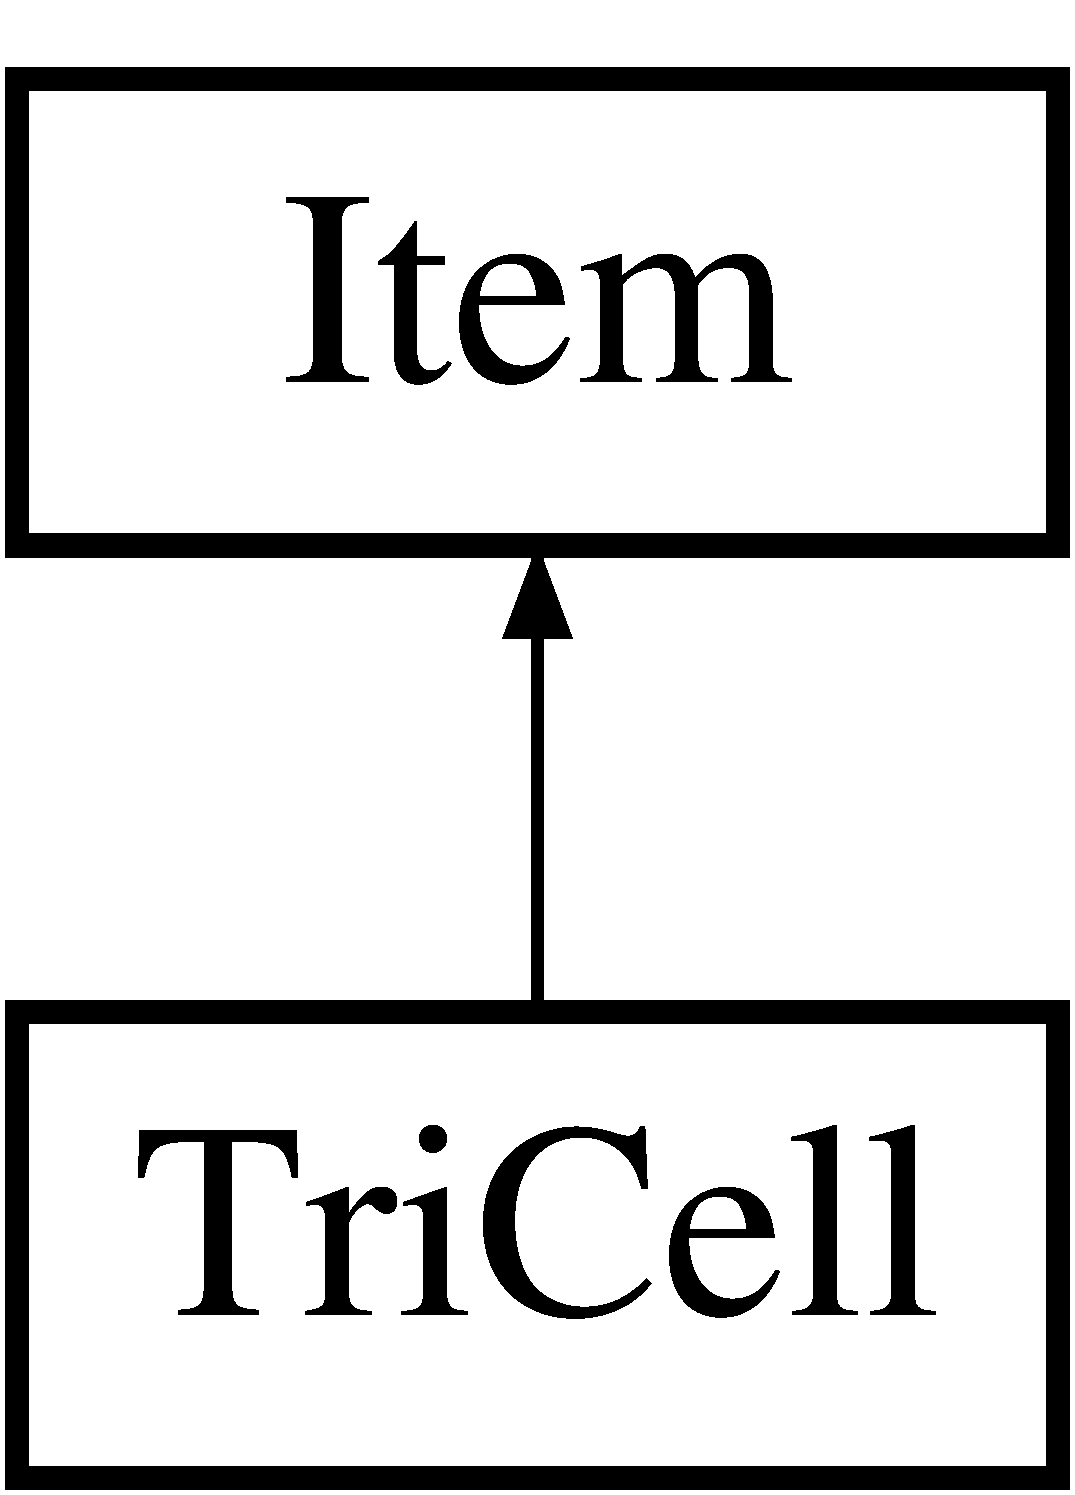
\includegraphics[height=2.000000cm]{classTriCell}
\end{center}
\end{figure}
\subsection*{Signals}
\begin{DoxyCompactItemize}
\item 
\hypertarget{classTriCell_a2db68cecb601d02fe73637ec5b5f3fb9}{void \hyperlink{classTriCell_a2db68cecb601d02fe73637ec5b5f3fb9}{toggle} (string new\-State, var mouse)}\label{classTriCell_a2db68cecb601d02fe73637ec5b5f3fb9}

\begin{DoxyCompactList}\small\item\em called when the state should be toggled (by clicking in the cell) \end{DoxyCompactList}\end{DoxyCompactItemize}
\subsection*{Public Member Functions}
\begin{DoxyCompactItemize}
\item 
\hypertarget{classTriCell_aae2f77800d2e5220e8e248a8e9dff234}{void {\bfseries toggle\-State} ()}\label{classTriCell_aae2f77800d2e5220e8e248a8e9dff234}

\end{DoxyCompactItemize}
\subsection*{Properties}
\begin{DoxyCompactItemize}
\item 
\hypertarget{classTriCell_af983c3fac0faae45c732ee4957b1bd11}{alias \hyperlink{classTriCell_af983c3fac0faae45c732ee4957b1bd11}{text}}\label{classTriCell_af983c3fac0faae45c732ee4957b1bd11}

\begin{DoxyCompactList}\small\item\em A text displayed within the cell. \end{DoxyCompactList}\item 
bool \hyperlink{classTriCell_a0be9a37b36e9ef3979ad775469415e69}{auto\-Toggle}
\end{DoxyCompactItemize}


\subsection{Detailed Description}
A styled cell with three different possible states. 

This component is functional similiar to a tri-\/state check box. The states are indicated with three different colors, the cell has a hover animation. The user can read and set the component's state with the {\ttfamily state} property. Three values are allowed\-: -\/{\ttfamily \char`\"{}off\char`\"{}}\-: indicates that the cell is inactive -\/{\ttfamily \char`\"{}on\char`\"{}}\-: indicates that the cell is active -\/{\ttfamily \char`\"{}mixed\char`\"{}}\-: indicates that the cell state is unknown 

\subsection{Property Documentation}
\hypertarget{classTriCell_a0be9a37b36e9ef3979ad775469415e69}{\index{Tri\-Cell@{Tri\-Cell}!auto\-Toggle@{auto\-Toggle}}
\index{auto\-Toggle@{auto\-Toggle}!TriCell@{Tri\-Cell}}
\subsubsection[{auto\-Toggle}]{\setlength{\rightskip}{0pt plus 5cm}bool Tri\-Cell\-::auto\-Toggle}}\label{classTriCell_a0be9a37b36e9ef3979ad775469415e69}
Set this to {\ttfamily true} if clicking in the cell should toggle the component's state. 

The documentation for this class was generated from the following file\-:\begin{DoxyCompactItemize}
\item 
/home/stoef/qt/projects/ddt/ddt/qml/ddt/Tri\-Cell.\-qml\end{DoxyCompactItemize}

%--- End generated contents ---

% Index
\newpage
\phantomsection
\addcontentsline{toc}{chapter}{Index}
\printindex

\end{document}
